\chapter{Développements logiciels}\label{chap:dev}
\minitoc

Ce chapitre présente les différents outils développés pour répondre aux objectifs présentés dans la \autoref{sec:dev_intro}. La \autoref{sec:dmlmem} et la \autoref{sec:kg} présentent deux outils permettant de caractériser le système mémoire et la capacité de calcul d'une architecture. Ensuite, la \autoref{sec:yamb} et la \autoref{sec:oprofile} présentent deux outils de suivi de performance pouvant être utilisés pour suivre l'utilisation du bus mémoire ainsi que pour extraire et caractériser les boucles critiques (\textit{hot spots}) d'une application.


\section{Introduction} \label{sec:dev_intro}


\subsection{Motivations}
%%%%%%%%%%%%%%%%%%%%%%%%%%%%%%%%%%%%



- Résumer la partie précédente, état de l'art etc.\\


\subsection{Objectifs}
%%%%%%%%%%%%%%%%%%%%%%%%%%%%%%%%%%%%




\subsection{Travaux existants}\label{sec:dev_existant}
%%%%%%%%%%%%%%%%%%%%%%%%%%%%%%%%%%%%

\subsubsection{Les outils de monitoring}

- Critique de l'existant\\


\subsubsection{Les benchmarks}

    Un objectif des benchmarks est de mesurer les performances maximales atteignables par une plate-forme. Ainsi, il est possible de quantifier la performance d'une application réelle en la comparant à cette première valeur. Le système mémoire étant le goulot d'étranglement de la performance d'une majorité d'application, de nombreux travaux ont été réalisés pour sa caractérisation et son optimisation. Un benchmark très connu (STREAM) permet de mesurer la bande passante maximale atteignable par 4 kernels de calculs différents. Il est donc possible d'utiliser ces résultats pour analyser la performance d'applications utilisant les mêmes familles d'algorithmes.



    \paragraph{STREAM}
        Le benchmark STREAM est surement un des benchmarks les plus connus et les plus utilisé au monde. Il a été développé et est maintenu par John McCalpin surnommé "Dr. Bandwidth". Le benchmark mesure la bande passante soutenanble pour quatre noyaux vectoriels simples. Les résulats sont donnés en GB/s et contiennent à la fois les opérations de lecture et d'écriture. Pour ces quatre opérations STREAM fonctionne en générant un tableau de nombres aléatoires d'une taille spécifiée (qui est ensuite stocké en RAM) et effectue quatre types d'opérations: \textit{copy, scale, add, triad}.  Le benchmark utilise \textit{OpenMP} pour utiliser la totalité des coeurs disponibles. Ces différents tests étaient à l'origine destinés pour caractériser la performance des architectures vectorielle. La performance mémoire pouvait alors varier d'une opération à l'autre. Aujourd'hui, la performance calculatoire des architectures n'est plus la contrainte principale et les quatre micro-benchmark obtiennent des performances équivalentes. Il est généralement accepté que la mesure donnée pour l'opération de \textit{triad} correspond à la bande passante maximale atteignable par l'architecture. On remarque que le noyeau de calcul du \textit{triad} est relativement simple et ne consiste qu'en la lecture de deux éléments et l'écriture du résultat. Les applications réelles utilisant des motifs d'accès bien plus complexes, cette mesure n'est pas représentative de la performance réellement atteignable par celles-ci \footnote{\url{https://www.intel.ru/content/dam/doc/white-paper/resources-xeon-7500-measuring-memory-bandwidth-paper.pdf}}
        

    \paragraph{lmbench} 
        Le benchmark \textit{lmbench}\cite{Staelin2004} a été développé par deux ingénieurs des HP Labs d'Israel en 2004. Ce code est en fait une suite de micro-benchmark permettant de mesurer la performance de plusieurs aspects d'une architecture: lecture d'un jeu de données, ouverture de fichiers, création de pipe, fréquence mémoire, taille d'une ligne de cache, taille de la TLB, bande passante mémoire (Stream). L'ensemble des codes peut être exécuté pour caractériser la mémoire d'un système partagé ou distribué \cite{Staelin2002}.
        \textit{Lmbench} facilite l'ajout de nouveau micro-benchmarks et mesure leur performance en donnant la latence par instruction et le débit mémoire. Le framework s'occupe de leur exécution pour atteindre des mesures de performances ayant une performances d'au moins 1\%. Écrit en ANSI-C et respectant la norme POSIX le benchmark a été développé pour maximiser sa portabilité. Cependant, sa compilation sur des architectures récentes peut être plus difficile \cite{Yotov2004}. En raison de son incapacité à mesurer les performances du cache distant et les transactions de cohérence du cache, le benchmark \textit{x86-membench} benchmark \cite{Molka2017b} a été développé pour supporter la mesure de la bande passante et de la latence du cache local ou distant mais aussi de la mémoire. Le benchmark n'utilise aucune méthode de parallélisme empêchant une caractérisation poussée des architectures modernes. 
        
    
    \paragraph{P-ray} 
        Pour remédier à l'incapacité de \textit{lmbench} de caractériser les plateformes multi-coeurs, le benchmark P-ray a été développé \cite{Duchateau2008}. Pour cela il étend les micro-benchmarks existant pour trouver le niveau des caches partagés, la topologie d’interconnexion, la bande passante effective ou la taille des blocs pour la gestion de cohérence des caches. Pour éviter les optimisations du compilateur (\textit{pointer chaising}), le benchmark utilise un système de liste chaînée lors de l'initialisation. Les résultats obtenus sont eux très précis et s'approchent souvent des maximums théoriques attendus.

    \paragraph{X-Ray} X-RAY \cite{Yotov2004} est un \textit{framework} utilisé pour implémenter des micro-benchmark destinés à mesurer des paramètres utile pour l’auto-optimisation. Pour cela il génère plusieurs benchmark gràce à un framework \textit{Nano-benchmark Generator}. Cette génération est dynamique car les benchmarks à générer varient en fonction de ceux déjà exécutés. Par exemple, le calcul de latence à besoin de connaître la fréquence du processeur pour donner un résulat en cycles

   Il existe de nombreux benchmarks permettant de caractériser différentes parties du système mémoire: les accès mémoires concurrents de systèmes multi-processeurs\cite{Mandal2010}, polices de mappage mémoire des systèmes NUMA \cite{Diener2015}, prédiction de la bande passante mémoire en fonction du placement des coeurs \cite{Wang2016a}, caractérisation de la hiérarchie mémoire \cite{Cooper2011}.
    
    The real problem is that the current synthetic benchmarks do not always show the strengths of all platforms thus not even allowing some CPUs to be considered for the application benchmarking.
    
    
\subsection{Contributions}
%%%%%%%%%%%%%%%%%%%%%%%%%%%%%%%%%%%%

- Délimiter les besoins auxquels nous répondons\\
- Motiver notre façon de développer\\

    Ces outils sont destinés aux développeurs soucieux de comprendre précisément la performance de son code. Pour réaliser cette analyse, il doit avoir accès au code source ainsi qu'aux compteurs responsable de l’activité du bus mémoire.
    
    Nous avons développé ces outils pour qu'ils soient aussi simple que possible répondant chacun à une question simple. Contrairement à d’autres outils déjà existant, il ne s'agit pas d’un gros outils permettant de tout faire. Leur efficacité réside dans la faculté de l’utilisateurs de les utiliser indépendamment pour mener son travail d'analyse

    Tous les outils que nous développons sont distribués en Open Source pour que le développeur puisse les modifier, se les approprier et réaliser des modifications pour ses propres besoins mais aussi pour les adapter sur des plateformes pas encore supportés.
    
    Beaucoup d’outils permettent de récupérer de nombreuses informations à travers les hardware counters. Cependant, il est souvent très difficile d’en tirer des conclusions: un grand nombre de miss dans le cache ne veut pas forcément dire que le code n’est pas efficace.
            --> les outils sont efficaces avec la bonne méthodologie
     
    La simplicité de ces outils doit permettre aux programmeurs de s’approprier le code pour l’adapter à ses besoins spécifiques 
    
    - Présenter ce chapitre\\


https://patentimages.storage.googleapis.com/f6/6c/60/8d079cef591498/US8225291.pdf

    - To bridge the productivity gap between hardware complex ity and Software limitations of current and next-generation high performance computing systems, performance tools should allow users at any level of experience to conduct performance analysis and tune Scientific applications. Tradi tional performance tools, however, offer little support for the non-expert user. Thus, non-expert users must seek the assis tance of performance tuning experts to improve application performance on their systems. While these tuning experts may improve application performance and help a few non expert users, the number of such experts is very limited. Consequently, many non-expert users do not have access to these experts.
    
    - Without the support of effective performance tools, users of these high performance computing systems will see this productivity gap continue to grow. Performance tools need to simplify the complexity of performance tuning and apply automatic, intelligent, and predictive technologies to mitigate the burden on today's Scientists and programmers. Currently, no solutions exist that automate and simplify the performance analysis and tuning cycle. The only known solutions for determining application performance bottlenecks today are Solutions that involve manual intervention by users.
    
    
https://patents.google.com/patent/US9032375B2/en
    - During performance analysis, an analyst determines a computer program's behavior based upon information gathered as that program is executed by a processor of a computer. For example, the analyst determines sections of code of the computer program that the processor is running inefficiently, such as sections of code that are taking longer than expected to execute and/or occupying more memory than expected. 
    
    
https://patents.google.com/patent/US9111032B2/en  
    -A bottleneck is a region of a program (e.g., program code) where significant execution time is spent. Typically, software developers use a profiling tool to collect program execution profiles such as the timing information for each method, routine, process, etc. With the help of such a profiling tool, the developer can sort, e.g., methods by the time spent on them. The methods that consume an amount of time greater than a threshold defined by, e.g., the developer may be treated as bottlenecks. However, the effectiveness of this approach depends on the program's runtime characteristics. Many programs, such as large enterprise commercial applications, do not have obvious bottlenecks. Therefore, their profiles contain a large amount of routines, processes, or methods where the execution time is spent relatively evenly (e.g., within a threshold). This type of profile is often referred to as a “flat profile” because no method dominates the execution time.
    
    
https://patents.google.com/patent/US9753731B1/en
    - herefore, execution of a program code may suffer from unpredictability and uncertainty. A user may not be able to expect consistency or predictability of performance among repeated executions of even the same program code on the same hardware. Moreover, a user may not be able to predict the performance of a program code on a new hardware system, even if the user measures the performance on a previous hardware system. For example, executing a program code on a new processor with twice the speed of a previous processor may not result in reducing the total execution time by half.
    
    - Such uncertainties and unpredictabilities may cause practical or financial hardships to users. For instance, in some performance sensitive applications, a user may err on the side of caution by using expensive hardware that has a much higher speed than the minimum required hardware for meeting the performance requirements. Alternatively, a user may not be able to predict the performance of the execution within some uncertainty limits. Adding predictability and certainty to the execution of a program code will reduce such hardships.
    
    
https://patents.google.com/patent/US8639697B2/en
    - The invention recognizes that, for many application programs that comprise functions, hotspots may not be at an instruction, function or module level, but at instruction blocks (instruction clusters) that are, for example, larger than one instruction and smaller than a function/module. Furthermore, besides hotspots, there may be code areas with large instruction blocks that are intensively executed even though each instruction may only consume a few of cycles. Such code areas may not comprise any hotspot, but cover a significant large address span and have performance improvement potential as well. Herein, these areas are also referred as to large warm areas. Although large warm areas may have room for optimization, they are prone to be omitted by existing instruction-sorting performance analysis tools, and can not be identified within the sorted list of instruction, function or module based performance statistics provided by those tools.
\newpage

\section{DML MEM: benchmark mémoire}\label{sec:dmlmem}

    La section suivante présente un benchmark mémoire appelé \textit{Demonstrate Memory Limit} ou \textit{DML\_MEM}. Cet outil permet de vérifier le bon comportement de la hiérarchie mémoire lors d'accès mémoire à un jeu de donnée par sauts de taille constante. 

    

    \subsection{Motivations}
    %%%%%%%%%%%%%%%%%%%%%%%%%%%%%%%%%%%%%%%%%%%%%%%%%%%%%%
    
        L'industrie de la recherche pétrolière est un grand consommateur de calculs haute performance. Les applications utilisées utilisent des algorithmes de Stencil qui impliquent des accès mémoire réguliers mais non contiguës par \textit{sauts} aussi appelés \textit{strides}. D'autres applications comme le calcul matriciel parcourent des matrices et génèrent des accès mémoire par saut de taille constante (multiple d'une taille d'une ligne). La \autoref{pic:dml_strides_acces_main} expose un exemple simple de tels accès. D'autres algorithmes peuvent réaliser ce genre d'accès par \textit{strides} comme les multiplications de matrices, les transformées de Fourrier ou le parcours d'un tableau de structures pour accéder à certains champs. Si les objets sont stockés continûment en mémoire, l'accès à un même champ de chaque objet réalise en réalité des accès mémoire par saut de taille fixes. 
        
        \begin{figure}[h!]
            \centering
                \begin{subfigure}[b]{0.25\linewidth}
                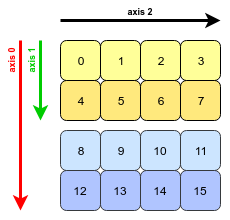
\includegraphics[width=\linewidth]{images/dml_strides_acces_matrix.png}
                \caption{Accès en ligne ou en colonne à une matrice.}
                \label{pic:dml_strides_acces_matrix}
                \end{subfigure}
            ~ %add desired spacing between images, e. g. ~, \quad, \qquad, \hfill etc. 
            %(or a blank line to force the subfigure onto a new line)
                \begin{subfigure}[b]{0.60\linewidth}
                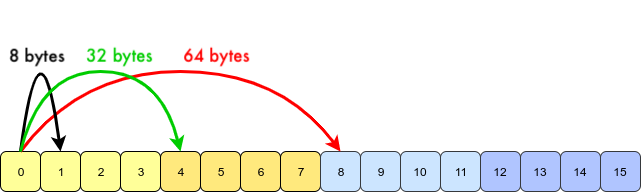
\includegraphics[width=\linewidth]{images/dml_strides_acces.png}
                \caption{Les accès en ligne ou en colonne implique des sauts en mémoire de différentes tailles.}
                \label{pic:dml_strides_acces}
                \end{subfigure}
            \caption{Exemple d'une application réalisant des accès en colonne à une matrice. Ces accès impliquent en réalité des sauts entre les adresses mémoire utilisées.}\label{pic:dml_strides_acces_main}
        \end{figure}
        % \subsubsection{Motivations}
    
    
        La grande majorité de ces applications ne réalisent pas suffisamment de calculs sur une donnée transférée pour masquer le temps de son accès mémoire. Ce déséquilibre de performance de l'architecture limite la performance de ces codes par celle du bus mémoire. 
        Pour ces applications, il est primordiale que l'architecture soit capable d'anticiper le maximum des accès mémoire grâce à son matériel de pré-lecture mémoire (\textit{memory prefetcher}). Les pré-lecteurs mémoire sont conçus pour anticiper les accès avant qu'ils ne soient réalisés pour réduire la latence d'accès. Lorsque les accès sont simples (taille régulière, proches en mémoire) la majorité des architectures modernes obtiennent de très bonnes performances. Cependant, les accès par sauts peuvent être grand (supérieurs à plusieurs lignes de cache) et lorsque de multiple accès sont réalisés en concurrence, le pré-lecteur peut rencontrer des difficultés à les anticiper. 
    
        

    \subsubsection{Objectifs}
        
        Pour vérifier la bonne performance d'une architecture pour une application donnée il n'est pas suffisant de vérifier que le bus mémoire est saturé. Pour l'illustrer, plusieurs expérimentations sont réalisées dans le \autoref{chap:methodo}. Ainsi, le benchmark \textit{DML\_MEM} a été élaboré pour prouver l'efficacité du système mémoire pour les applications utilisant des motifs d'accès par \textit{strides}. 
    
        Le premier objectif du benchmark \textit{DML\_MEM} est de caractériser la micro-architecture pour des applications utilisant des motifs d'accès par \textit{strides}. En mesurant ses performance il est ensuite possible de prouver l’efficacité de l’utilisation du sous-système mémoire pour une application étudiée. 
        
        Le deuxième objectif est d'attirer l'attention du programmeur sur la complexité des architectures et de son impact sur les performances d'un code. En appréhendant cette complexité, il sera plus simple pour le programmeur d'apporter les bonnes modifications à son codes pour tirer la pleine performance du bus mémoire.
        
        Une autre utilisation de notre outil peut aussi être réalisée par les concepteurs d'architectures qui veulent vérifier le bon fonctionnement du système mémoire pour ce type d'application. En effet, en utilisant ce benchmark nous avons trouvé certains dysfonctionnements majeurs dans un accélérateur prévu pour ce type d'applications. Grâce à notre outil, nous avons pu prouver que les performances théoriques de la plate-forme n'étaient pas accessibles par l'application. 
    
    
    \subsubsection{Comparaison avec l'existant}
    %%%%%%%%%%%%%%%%
        L'étude des différents benchmarks existant est réalisé dans la \autoref{sec:dev_existant}. Le seul outil s'approchant de notre démarche est le benchmark DISBench \cite{disbench}. Cependant, il ne bénéficie d'aucune méthode solide de vérification de la performance comme celui implémenté par \textit{DML\_MEM}. De plus, il n'est en aucun cas prévu pour faciliter le tests de multiple tailles de strides sur différentes tailles de jeux de données. Le code n'est plus maintenue depuis 6 ans et ne peut pas être exécuté sans erreur lors de l'exécution. Au moment de l'écriture de cette thèse, nous ne sommes au courant d'aucun outil permettant de remplir les objectifs fixés dans le section précédente. 


\subsection{Le benchmark DML\_MEM}
%%%%%%%%%%%%%%%%%%%%%%%%%%%%%%%%%%%%%%%%%%%%%%%%%%%%%%
    Le motif d'accès par \textit{stride} est donc très courant dans le calcul haute performance. La distance entre deux accès peut varier d'une application, ou d'un jeu de données, à l'autre. Pour caractériser les plate-formes pour ces applications il est donc nécessaire de posséder un benchmark paramétrable permettant de faire varier la taille du jeu de données et du saut. Cette section présente comment est conçu le benchmark \textit{DML\_MEM} et comment il peut être utilisé. Grâce à de nombreuses options, différentes partie de la micro-architectures peuvent être testée: caches, TLB, bus mémoire.


    \subsubsection{Concept}
    %%%%%%%%%%%%%%%%
        
        Le principe du benchmark est d'accéder à un tableau en utilisant différentes tailles de strides. Pour chaque stride une mesure de performance est réalisée. Une fois toutes les tailles de stride mesurée, le benchmark augmente la taille du jeu de données utilisé (voir \autoref{pic:dml_stride_intro}). La vitesse d'évolution de la taille des strides et du jeu de données peut être paramétrée. Les accès peuvent être réalisés en lecture ou en lecture/écriture.
       
        \begin{figure}[h!]
        \center
        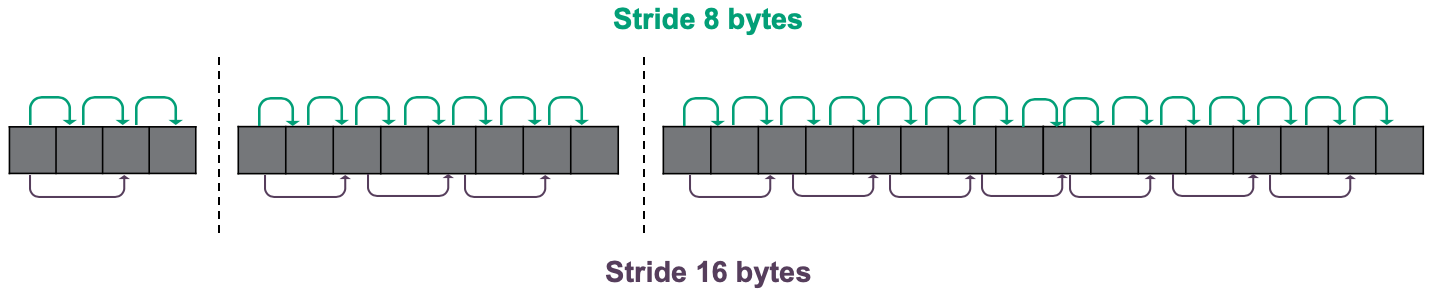
\includegraphics[width=14cm]{images/dml_stride_intro.png}
        \caption{\label{pic:dml_stride_intro}Évaluation de la performance de deux tailles de stride (8 et 16 bytes) sur trois jeux de données de tailles différentes.}
        \end{figure}

    
    \subsubsection{Développement}
    %%%%%%%%%%%%%%%%

        Le benchmark se déroule en deux étapes: la configuration et son exécution.
        Lors de la configuration les différents paramètres nécessaires pour l'exécution du benchmark sont extraits de la ligne de commande ou utilisent, le cas échéant, des valeurs par défaut. Les différentes versions du benchmark (mode d'accès, taille du déroulement des boucles) sont toutes compilées, l'initialisation utilise un pointeur de fonction vers la bonne version requise par l'utilisateur. Ensuite, le jeu de données est initialisé (voir \autoref{sec:dml_init}). 
        La deuxième étape consiste à exécuter le benchmark et à mesurer ses performances. Pour une taille de jeu de donnée et une taille de stride, la bande passante effective maximale, minimale ou moyenne est mesurée et affichée. Pour cela, le benchmark mesure le temps nécessaire pour réaliser le noyau de calcul. Celui ci, renvoie le nombre d'accès réalisés grâce à l'initialisation du tableau durant la première étape. 
            \begin{verbatim}
time1 = get_micros();
num_ops = p->m_BENCHMARK();
time2 = get_micros();
bande_passante = calcul_bw(num_ops, time2 - time1);
            \end{verbatim}
            
        Ces mesures sont affichées au fur et à mesure de l'avancée du benchmark ainsi que dans un fichier de \textit{log}. Ce fichier, peut ensuite être utilisé par un script pour afficher l'évolution de la performance de chaque stride en fonction de la taille du jeu de donnée. 
            
\begin{verbatim}
>./dml --type read --cacheline 64 --matrixsize 10000 --stride 8,64,256
...
Stride  S   ->          8         64        256
Value       ->    AVERAGE    AVERAGE    AVERAGE
       7.0 KiB     117.46          -          -
      81.0 KiB     114.29      88.24      74.12
      76.3 MiB      80.87      13.41       8.61
       7.5 GiB      80.35      13.11       7.18
...
\end{verbatim}

  

    \subsubsection{Les options}
    %%%%%%%%%%%%%%%%
        Le benchmark \textit{DML\_MEM} accepte de nombreuses options. Grâce à celles-ci différentes configurations peuvent être utilisées pour tester différents scénarios sur différentes parties de la micro-architecture. Nous décrivons ici les options les plus utiles pour l'utilisateur. Les nombreuses options peuvent être affichées avec l'option \verb|--help|.
        
        
        \paragraph{-{}-stride, -{}-minstride, -{}-maxstride, -{}-stridemode} Ces quatre premières options permettent de définir quelles sont les différentes stride à utiliser pour réaliser les mesures. La première d'entre elles, permet à l'utilisateur de choisir une ou plusieurs à réaliser. Pour cela, une liste de taille de strides séparées par des virgules doit être entrée. Les trois dernières options, permettent de générer automatiquement des strides à utiliser dans un intervalle $[min, max]$. L'option \verb|--stridemode| peut être utilisée avec les valeurs \textit{even} et \textit{odd} pour décaler les strides ainsi générées. Cela permet d'éviter des strides utilisant seulement des multiples de deux, pouvant être affectées par certaines caractéristiques de la micro-architecture (taille ligne de cache, taille des caches...). 
        
        \paragraph{-{}-matrixsize, -{}-minlog, -{}-maxlog, -{}-steplog, -{}-log} Ces 5 options permettent de définir la taille des jeux de données à utiliser. Leur taille évolue plus ou moins rapidement en fonction de la valeur de \verb|--steplog| jusqu'à atteindre la taille \verb|max| ou bien celle de la matrice donnée avec l'option \verb|--matrixsize|. L'option \verb|--log| permet de donner la même valeur à \verb|min| et \verb|max| pour ne réaliser la mesure que sur une taille de jeux de données. S'il est utilisé avec la valeur $0$, le benchmark utilise la totalité du tableau. Couplées avec l'option \verb|--stride|, ces deux options permettent d'utiliser le benchmark pour n'accomplir qu'une seule mesure: un jeu de donnée, une stride.
        
        Ces 9 premières options sont les options principales du benchmark. Elles permettent de réaliser une multitude de mesure: performance des niveaux de caches, performance de la mémoire, fiabilité du pré-chargement, mesure de la taille d'une ligne de cache. Dans la \autoref{sec:dml_bad_stride} nous montrons comment ces options peuvent être utilisées pour identifier des tailles de strides ayant de mauvaises performances
    
    
        \paragraph{-{}-type, -{}-unroll, -{}-mode} Ces trois options permettent de choisir le benchmark à utiliser. L'option \verb|--type| permet de réaliser les accès en lecture ou en lecture/écriture. La deuxième option permet d'appliquer l'optimisation du déroulement de boucle dont les différentes versions (déroulement de 2 à 64 fois) ont été programmées manuellement. La troisième option permet de choisir le mode d'accès comme par exemple l'utilisation de différents pointeurs pour réaliser plusieurs accès notamment lorsque l'option \verb|--unroll| est utilisée. L'analyse de la performance de ces options est réalisée dans la \autoref{sec:dml_unroll}.

        \paragraph{-{}-hugepages} Cette option permet d'allouer la mémoire pour le jeu de données en utilisant des pages de 2 MiB contre 4 KiB habituellement. La caractérisation des pages larges est réalisée dans la \autoref{sec:dml_large_page}.
        
        \paragraph{-{}-annotate} Cette option est utilisée lorsque l'activité du bus mémoire est mesurée avec l'outil YAMB (\autoref{sec:yamb}). Le benchmark ajoute une trace lors de chaque nouvelle stride utilisée et lorsque la taille du jeu de données change. Grâce à cette option il est possible de corréler l'activité du bus avec une configuration particulière du benchmark. Cette option est utilisée dans la \autoref{sec:dml_cache_ok} pour mesurer l'activité du bus mémoire lorsqu'un jeu de donnée de la taille du dernier niveau de cache est utilisée. 

        \paragraph{Version parallèle} La dernière configuration du benchmark est la version parallèle utilisant MPI. Celle-ci doit être générée grâce à l'outil \textit{cmake} et la commande \verb|cmake -DOPT_BUILD_MPI=ON|. Grâce à cette version, plusieurs coeurs peuvent exécuter la même version du benchmark. Cette version du benchmark nous permet dans la \autoref{sec:dml_saturation} de mesurer l'évolution du débit mémoire lorsque des coeurs sont ajoutés.
        
    
    \subsubsection{Validation des résultats}
    %%%%%%%%%%%%%%%%

    Une grande difficulté lors de l'élaboration d'un benchmark est de s'assurer que la performance mesurée est bien celle du code attendue. En effet, le compilateur peut appliquer certaines optimisations pour accélérer l'application. Ensuite, l'architecture elle même peut se rendre compte de l'artificialité du code et en court-circuiter une partie. Dans les deux cas, le problème est que la mesure de la performance ne rend pas compte de la réalité du code et de la mesure attendue par le programmeur. 
    
    Pour éviter ces deux pièges, le benchmark \textit{DML\_MEM} initialise le jeu de données avec deux valeurs suivant le type de l'accès voulu (lecture ou lecture/écriture). Lorsque le benchmark utilise des accès en lecture, le jeu de données est initialisé avec la valeur \textbf{1} car chaque lecture occasionne un transfert sur le bus mémoire. 
    Lorsque le benchmark utilise le mode de lecture/écriture, le jeu de données est initialisée avec la valeur \textbf{2}. Chaque ligne doit être lue puis réécrite occasionnant deux passages sur le bus mémoire. Pour chaque accès la valeur contenue dans le tableau est stockée dans une variable de compteur.  L'utilisation de chaque valeur pour l'ajouter au compteur empêche le compilateur et l'architecture d'appliquer certaines optimisations. A la fin de l'exécution, le benchmark retourne cette variable permettant de compter le nombre total d'accès effectivement réalisés.
    

    
    
    
    
    
    
    
    
\subsection{Résultats}
%%%%%%%%%%%%%%%%%%%%%%%%%%%%%%%%%%%%%%%%%%%%%%%%%%%%%%

    Dans cette section nous présentons les principaux résultats obtenus avec le benchmark DML\_MEM présenté précédemment. L'objectif est de montrer au lecteur les différentes mesures rendu possible par l'utilisation de l'outil. Les tests sont principalement réalisés sur l'architecture des processeurs Intel Skylake. 


    \subsubsection{Choix du compilateur}
    %%%%%%%%%%%%%%%%
    
        Contrairement au benchmark du générateur de kernel (voir \autoref{sec:kg}), le code de DML\_MEM n'est pas écrit directement en assembleur. La qualité du compilateur peut donc avoir un impact significatif sur ses performances. Avant de réaliser plus d'expérimentations, nous avons testé deux compilateurs (GCC 8.2 et ICC 19.0) avec différents drapeaux de compilation. Avec d'ancienne version de GCC (telle que la version 4.8), nous avons mesuré une amélioration d'un facteur deux en utilisant les drapeaux \verb|-O3 -march=skylake-avx512|. Le compilateur ayant reçu de nombreuses améliorations depuis, nous n'avons trouvé aucun drapeau permettant d'améliorer les performances de ce dernier. Nous l'avons comparé avec la version 19.0 du compilateur d'Intel ICC couplé avec le drapeau \verb|-O3|. Les performances mesurées dans les différents niveaux de la hiérarchie mémoire sont présentées dans le \autoref{tab:dml_compiler}.

        \begin{table}[h!]
        \centering
        \begin{tabular}{|l|c|c|}
        \hline
        Perf. GB/s & GCC 8.2 & ICC 19.0 \\ \hline
        L1 & 58 & 310 \\ \hline
        L2 & 56 & 161 \\ \hline
        L3 & 26 & 26 \\ \hline
        Memory & 12.5 & 12.5 \\ \hline
        \end{tabular}%
        \caption{Performance du benchmark DML\_MEM compilé avec les compilateurs GCC et ICC mesurée en GB/s. Le drapeau d'optimisation \text{-O3} est utilisé dans les deux cas.}
        \label{tab:dml_compiler}
        \end{table}

        Lorsque le jeu de données tient dans le premier niveau de cache, nous avons mesuré des différences de performances du benchmark pouvant aller jusqu'à un facteur 8. Cet écart de performance entre les deux compilateurs se réduit lorsque la taille du jeu de données augmente. En effet, la performance du bus mémoire pour les deux compilateurs est équivalente. Nous expliquons cet écart de performance dans les premiers niveaux de cache par la mauvaise performance du code généré par le compilateur GCC. Le premier niveau de cache des processeurs Skylake est capable de fournir 128 octets par cycle, soit une bande passante de 345 GB/s. Le code généré par GCC ne parvient pas à utiliser plus de 58 GB/s. Nous avons mesuré que le benchmark compilé par GCC utilisé deux fois plus d'instructions que celui compilé par ICC. Le benchmark GCC n'est alors pas \textit{memory bound} mais \textit{compute bound}. La bande passante disponible se réduisant lorsqu'on remonte dans la hiérarchie mémoire, l'impact de la qualité du code est elle aussi réduite. Les performances du benchmark compilé par ICC étant toujours supérieures à celles produites par GCC, nous utiliserons le compilateur d'Intel dans les prochaines expérimentations. Lorsque de nouvelles versions sont disponibles ou que d'autres architectures sont étudiées nous conseillons de toujours tester les différentes versions de compilateurs avec les drapeaux de compilation adéquats.
    
    
    
    \subsubsection{Mesurer la taille d'une ligne de cache}
    %%%%%%%%%%%%%%%%
        Connaître la taille d'une ligne de cache de l'architecture est nécessaire pour obtenir les mesures correctes par le benchmark. Cette taille peut aussi être nécessaire lors du développement d'une application pour disposer les données de façon optimale. Nous montrons dans cette expérimentation comme celle-ci peut être retrouvée en utilisant le benchmark DML\_MEM. Pour cela, nous désactivons le \textit{memory prefetch} pour l'empécher d'anticiper le chargement d'une ou plusieurs ligne de cache avant son accès. Le jeu de données utilisé doit quand à lui plus grand que le dernier niveau de cache. La taille des lignes de cache des architectures modernes est généralement compris entre 32 et 256 bytes. Nous utilisons le benchmark pour mesurer la performance du système mémoire en utilisant des strides de puissance de 2 allant de 8 à 256 bytes. Les performances ainsi mesurées sont présentées dans le \autoref{tab:dml_cache_line}.
    
        \begin{table}[]
        \centering
        \begin{tabular}{|l|c|c|c|c|c|c|}
        \hline
        Taille de la stride (byte) & 8 & 16 & 32 & 64 & 128 & 256 \\ \hline
        Bande passante (GB/s) & 31.58 & 25.84 & 14.50 & 7.62 & 7.65 & 7.62 \\ \hline
        \end{tabular}%
        \caption{Pour un jeu de données de 1 GiB, mesure de la performance de plusieurs tailles de stride lorsque le pré-chargement mémoire est désactivé.}
        \label{tab:dml_cache_line}
        \end{table}
        
         L'interprétation de ces résultats doit être la suivante. Pour des strides de 64, 128 ou 256 bytes, la performance est la même. Il est important de rappeler que le benchmark mesure le débit mémoire atteint par l'application et non le trafic mémoire du bus. Ceci indique que pour ces trois cas, le processeur attend une ligne de cache pour réaliser un accès. Le prochain accès étant situé sur une autre ligne de cache, leur performance est équivalente. Lorsqu'une stride de 32 bytes est utilisée, la performance double, indiquant que la taille d'une ligne de cache est de 64 bytes. En effet, le processeur est capable de réaliser deux fois plus d'accès. Ceci est possible car lorsqu'un premier accès est réalisé sur une ligne de cache, le suivant le sera aussi. La donnée est alors déjà présente dans le cache L1. L'utilisation d'une stride de 16 bytes améliore encore la performance du benchmark sans doubler pour autant. En effet, comme dans la première expérimentation le code devient \textit{compute bound}. Le benchmark additionne des nombres flottants et la performance du code est alors limitée par l'ALU. 
    
    
    \subsubsection{Performances de différentes tailles de strides} \label{sec:dml_bad_stride}
    %%%%%%%%%%%%%%%%
        
        Un objectif principal de notre benchmark est de vérifier le bon comportement du processeur lors d'accès mémoire utilisant des sauts mémoire constant. Pour cela, nous avons développé un script qui permet d'exécuter le benchmark avec un grand nombre de strides et d'afficher leur performance dans un graphique. La \autoref{pic:dml_strides_bad} montre le résultat d'une telle exécution. Pour chaque stride et chaque taille de jeu de données une mesure est réalisée. Pour faciliter la lecture du graphique nous avons coloré les strides en fonction de leur tailles en allant du bleu (pour les strides les plus petites) au rouge (pour les plus grandes). Nous remarquons que les strides de grande taille (plusieurs MiB) ont de meilleurs performances que celle de petite taille. En effet, même pour des tailles de jeu de données de plusieurs centaines de mégaoctets (ne pouvant pas tenir dans le cache), le benchmark mesure des performances similaires à si le jeu de données se trouvait dans le cache. En réalité, pour des grandes tailles de strides, le jeu de données réellement utilisé par le benchmark peut être contenu dans les différents niveaux de cache. 
      
        \begin{figure}
        \center
        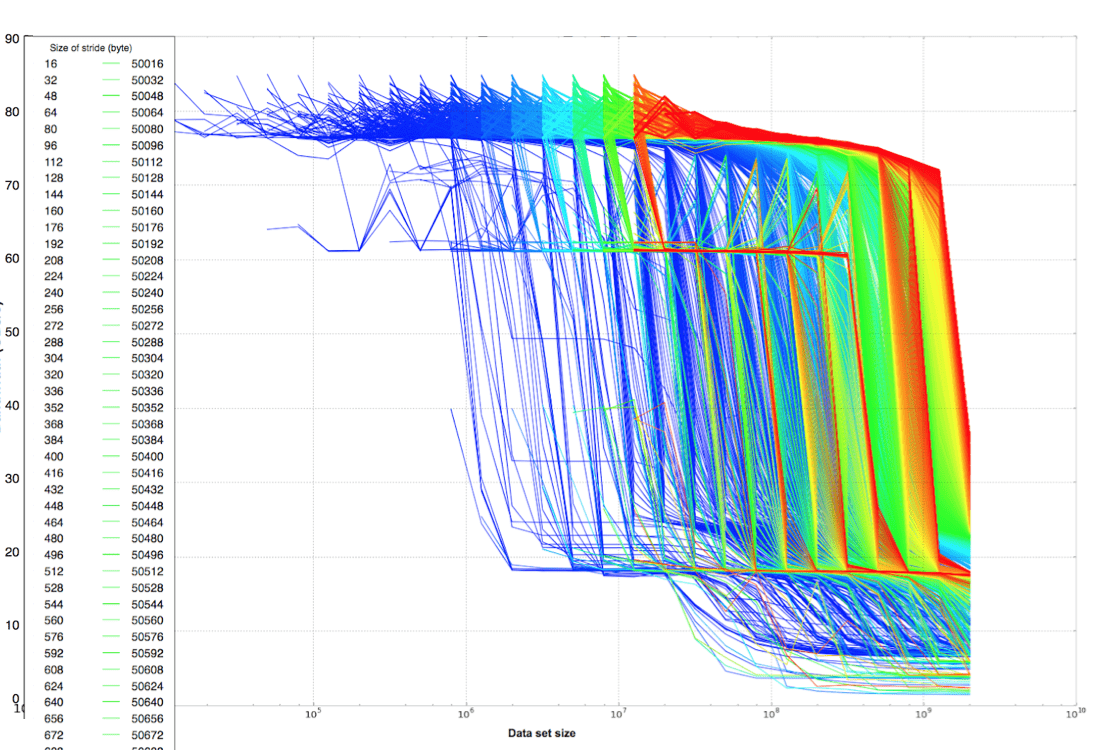
\includegraphics[width=12cm]{images/dml_strides_bad.png}
        \caption{\label{pic:dml_strides_bad} Performance du benchmark pour différentes tailles de strides (couleurs).  }
        \end{figure}
        
        Nous remarquons sur la \autoref{pic:dml_strides_bad} que certaines strides ont des comportements différentes que des strides de tailles proches (donc de couleurs proches aussi). En effet, des groupes de strides ont des performances bien plus faibles que d'autres et les mêmes résultats sont obtenus en utilisant des pages large pour réduire l'impact sur la TLB. Nous avons isolé certaines d'entre elles et reporté leur performance dans le  \autoref{tab:dml_bad_strides}. Pour réaliser ces mesures la commande suivante a été utilisée: 
        \begin{verbatim}
./dml --steplog 0.01 --unroll 8 --mode special --type read --cacheline 64 
      --stride 73704,73728,77816,77824,81928,81920 --measure 10 --matrixsize 10000
        \end{verbatim}
        
        
        \begin{table}[]
        \centering
        \begin{tabular}{|c|c|c|c|c|}
        \hline
        \rowcolor[HTML]{EFEFEF} 
        Taille de la stride (byte) & Bande passante (GB/s) & Nb. inst. & IPC & LLC Miss \\ \hline
        \rowcolor[HTML]{FFFFC7} 
        73704 & 24.54 & 690071400 & 0.34 & 21100474 \\ \hline
        \rowcolor[HTML]{FFFFC7} 
        73728 & 2.04 & 690064918 & 0.22 & 30612018 \\ \hline
        \rowcolor[HTML]{E8FFFE} 
        77816 & 24.53 & 688909428 & 0.33 & 21152403 \\ \hline
        \rowcolor[HTML]{E8FFFE} 
        77824 & 4.01 & 688905576 & 0.27 & 30144907 \\ \hline
        \rowcolor[HTML]{E6FFE6} 
        81928 & 24.76 & 690692156 & 0.33 & 21194483 \\ \hline
        \rowcolor[HTML]{E6FFE6} 
        81920 & 4.03 & 690693382 & 0.27 & 30794354 \\ \hline
        \end{tabular}%
        \caption{Différence de performance de trois couples de stride}
        \label{tab:dml_bad_strides}
        \end{table}
        
        
        Le benchmark qui utilise une \textit{mauvaise} stride est \textit{latency bound}. En effet, nous avons réalisé différentes mesures telles que le nombre de \textit{miss} du dernier niveau de cache ou l'activité du bus mémoire. On remarque que l'IPC est plus faible et que le nombre de \textit{miss} est lui plus élevé pour ces strides. L'analyse de l'activité du bus mémoire montre qu'il est loin d'être saturé. Si la ligne de cache n'est pas présente dans un des niveau de cache, et que le bus n'est pas saturé c'est que le processeur l'attend et n'a pas anticipé son manque (\textit{miss}). La question est alors de savoir pourquoi pour une certaine taille la ligne de cache est présente dans le cache et que pour une stride plus grande de quelques bytes elle n'y soit pas. L'explication vient de la taille des strides utilisées. Nous avons utilisé des strides de taille $ Stride_{n+1} = Stride_n + 16 bits$ avec $Stride_0 = 16 bytes$. En utilisant des tailles de multiple de 16 certaines d'entre elles génèrent des conflits avec la politique de remplacement de lignes de caches. Ainsi, certaines d'entre elles mettent la pression seulement sur une partie du cache, le rendant inefficace. Le processeur doit donc attendre pour une majorité des accès que la ligne de cache soit transféré depuis la mémoire rendant le code \textit{latency bound}.
        
        Nous avons ensuite réalisé la même expérimentation en décalant la taille des strides utilisées en commençant avec une stride minimale $Stride_0 =  8 bytes$. Ainsi, aucune stride utilisée n'est multiple de 32, et aucune d'entre elle obtient de performance inattendue (voir \autoref{pic:dml_strides_good}).
        
        
        \begin{figure}
        \center
        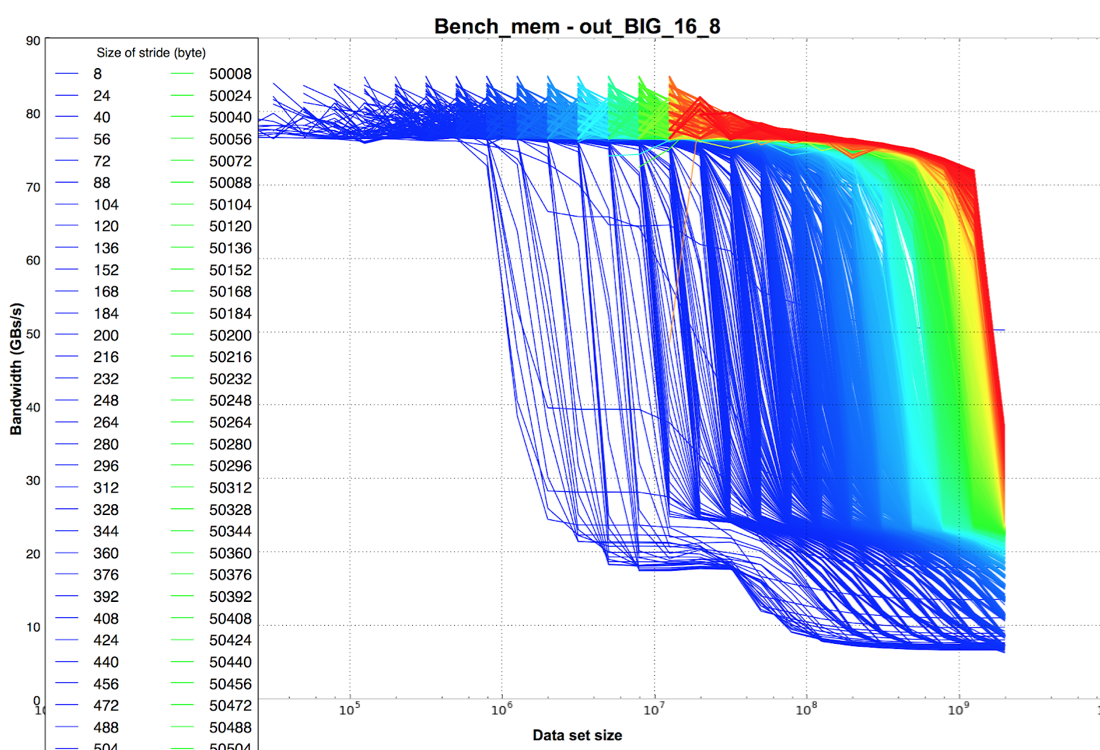
\includegraphics[width=12cm]{images/dml_strides.png}
        \caption{\label{pic:dml_strides_good} Performance du benchmark pour différentes tailles de strides (couleurs).  }
        \end{figure}
        
        À travers cette expérimentation, nous avons voulu montrer qu'un code aussi simple qu'il soit, peut avoir des performances inattendues. La complexité des architectures modernes est telle qu'elle peut avoir une incidence forte sur la performance des applications. Pour des strides aussi longues (plusieurs MiB), le \textit{memory prefetcher} ne semble pas arriver à anticiper ces accès. Si une application réalise ce type d'accès, le programmeur doit s'assurer de ne pas réaliser des strides de cette taille en ajoutant du \textit{padding} (remplissage) pour décaler artificiellement les données accédées. Une autre optimisation lors d'accès à certains champs d'objets contenus dans un tableau est de regrouper ces mêmes champs dans une structure spécifique. Ainsi, ces champs sont contiguës en mémoire. 
        
        
        

    \subsubsection{Saturation du bus mémoire}\label{sec:dml_saturation}
    %%%%%%%%%%%%%%%%
        Que ce soit pour notre modèle de performance ou d'autres de type \textit{Roofline}, il est nécessaire de connaître la bande passante maximale atteignable par un processeur. Pour cela, nous avons exécuté le benchmark en utilisant différents nombre de coeurs. Les résultats sont visible sur le graphique de la \autoref{pic:dml_bw_mpi}. Sur ce processeur, notre benchmark arrive à obtenir une bande passante mémoire maximale de 114 GB/s. La loi de Little ne permet pas à un seul coeur de saturer la totalité du bus mémoire. Nous montrons à travers cette expérimentation qu'il faut au moins 15 coeurs pour le saturer. Les coeurs supplémentaires ne permettent pas ensuite d'améliorer le débit mémoire car le bus est saturé. Pour des codes \textit{memory bound} il peut alors être intéressant d'en désactiver certains ou de ne pas investir dans des processeurs avec plus de coeurs. Nous présentons dans la \autoref{sec:dml_core_vs_freq} un script permettant de réaliser cette recherche du nombre minimal de coeurs permettant de saturer le bus mémoire. 
        
        \textit{TODO: comparaison avec STREAM}
        
        \begin{figure}
        \center
        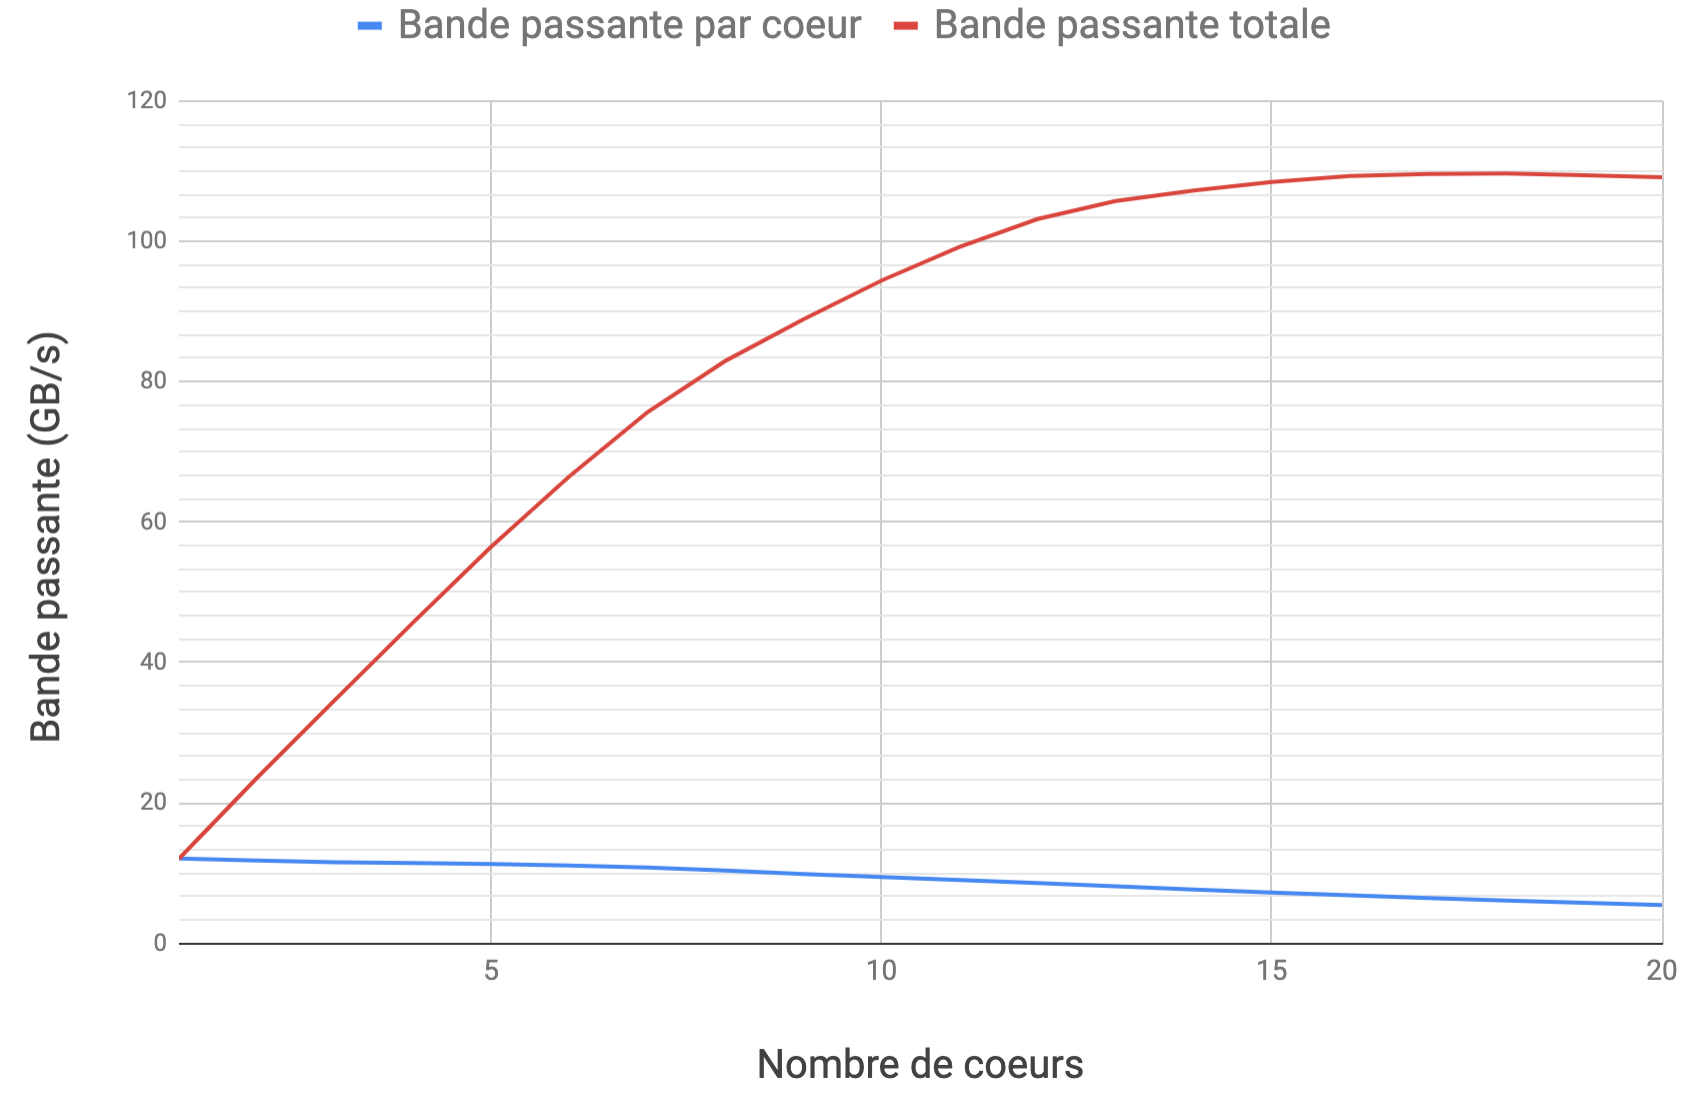
\includegraphics[width=10cm]{images/dml_bw_mpi.png}
        \caption{\label{pic:dml_bw_mpi} Bande passante mémoire atteinte pour différent nombre de coeurs}
        \end{figure}
        
    
    
    

    \subsubsection{Vérifier le bon fonctionnement des caches} \label{sec:dml_cache_ok}
    %%%%%%%%%%%%%%%%
        Les caches des architectures modernes se sont complexifiés et sont devenus très efficace pour accélérer les accès mémoires. Cependant, sur des architectures différentes que celles utilisées communément, il peut être intéressant de vérifier leur bon fonctionnement. Nous montrons dans cette expérimentations les tests pouvant être réalisés.
        
        La première vérification est de s'assurer de l'indépendant des caches propres à chaque coeur. Dans le cas des processeurs Skylake, les deux premiers niveaux sont privés à chaque coeur. Nous avons implémenté une option pour annoter la taille de niveau de cache sur le graphique final. Les résultats de deux exécutions sur 1 et 20 coeurs sont présentés sur la \autoref{pic:dml_cache}. La performance lorsque le jeu de donnée est contenu dans le cache L1 et L2 n'est pas impacté par l'utilisation d'autres coeurs. Les performances se dégradent lorsque le jeu de données commencent à remplir le dernier niveau de cache, commun à tous les coeurs. La même expérimentation peut être menée sur les différents cache L3 de plusieurs processeurs d'un même serveur.
        
        \begin{figure}
        \centering
            \begin{subfigure}[b]{0.47\linewidth}
            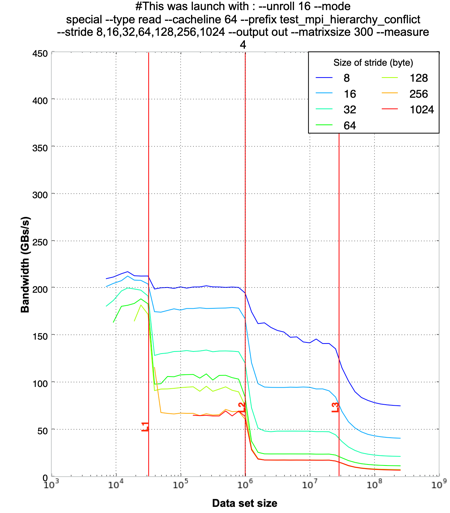
\includegraphics[width=\linewidth]{images/dml_cache_1core.png}
            \caption{1/20 coeur actif}
            \label{pic:dml_cache_1core}
            \end{subfigure}
        ~ %add desired spacing between images, e. g. ~, \quad, \qquad, \hfill etc. 
        %(or a blank line to force the subfigure onto a new line)
            \begin{subfigure}[b]{0.47\linewidth}
            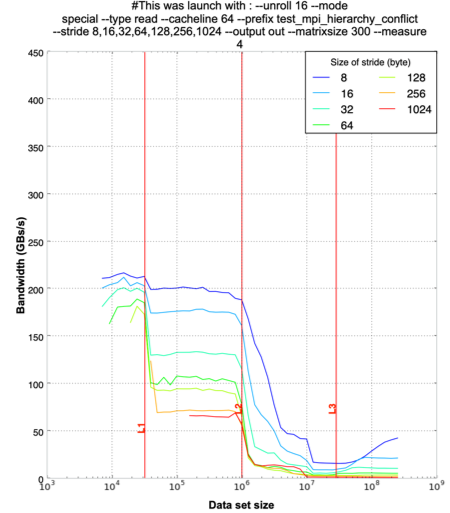
\includegraphics[width=\linewidth]{images/dml_cache_20core.png}
            \caption{20/20 coeurs actifs}
            \label{pic:dml_cache_20core}
            \end{subfigure}
        \caption{Performance du benchmark lorsqu'un ou la totalité des coeurs sont actifs. Les résultats montrent que les cache L1 et L2 ne sont pas affectés par l'utilisation d'autres coeurs.}\label{pic:dml_cache}
        \end{figure}
        
        Une deuxième expérimentation pouvant être menée au niveau des caches est la vérification du fonctionnement du cache L3. Pour cela, nous utilisons un jeu de donnée dont la taille évolue jusqu'à remplir le dernier niveau de cache.  En parallèle, nous mesurons l'activité sur le bus mémoire avec l'outil YAMB (voir \autoref{pic:dml_L3_sharing}). Cette expérimentation peut être réalisée avec les commandes suivantes:
        \begin{verbatim}
./monitoring_bw_main.sh --start
./dml --steplog 0.01 --unroll 2 --type read --cacheline 64 --stride 64  
      --matrixsize 100 --measure 1000 --minlog 6.1 --annotate log_mem.annotate
./monitoring_bw_main.sh --stop
        \end{verbatim}
        
         \begin{figure}
        \center
        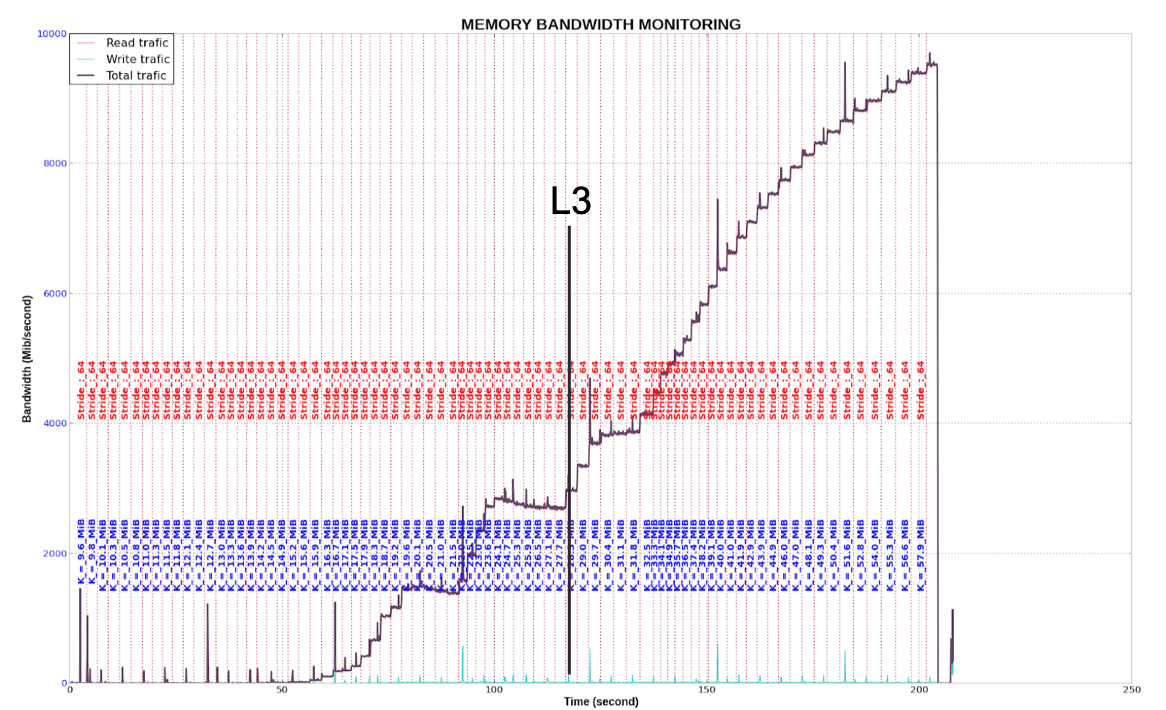
\includegraphics[width=14cm]{images/dml_L3_sharing.png}
        \caption{\label{pic:dml_L3_sharing} Évolution de l'activité du bus mémoire en fonction de la taille du jeu de donnée.}
        \end{figure}
        
        Nous montrons ainsi que pour un cache L3 de 28 MiB ne parvient pas à garder la totalité d'un jeu de donnée dépassant les 16 MiB. Au dela de cette taille, YAMB mesure de l'activité sur le bus mémoire pouvant atteindre les 3 GB/s pour un jeu de donnée de la taille du L3 (28MiB). 
        
        
        Cette mauvaise utilisation du cache peut être dû au phénomène de coloration de page discuté dans les expérimentations suivantes. Cette caractéristique impact la performance de chaque coeurs car certaines données sont éjectées du cache et génère un évènement de \textit{miss}. Nous avons réalisé une seconde expérimentation en utilisant deux jeux de données de 20 et 28 Mib. Pour chaque jeu, nous utilisons progressivement la totalité des coeurs. Le résultat présenté sur la \autoref{pic:dml_bw_cacheL3} montre que le phénomène de \textit{trash} est encore plus fort lorsque plusieurs coeurs sont utilisés. Le trafic généré atteint les 19 GB/s pour 6 coeurs se partageant un jeu de données de 28 MiB. Cependant, la performance entre les deux benchmark est identique, permettant de conclure du bon fonctionnement du \textit{memory prefetcher}. Si une architecture ne possède pas un composant aussi efficace il peut alors être intéressant de réduire la taille des jeux de données utilisés. Pour certaines optimisations, tel que le \textit{cache blocking}, nos expérimentations nous ont montrés que qu'utiliser 80\% de la capacité du dernier niveau de cache était le plus efficace.
        
        \begin{figure}
        \center
        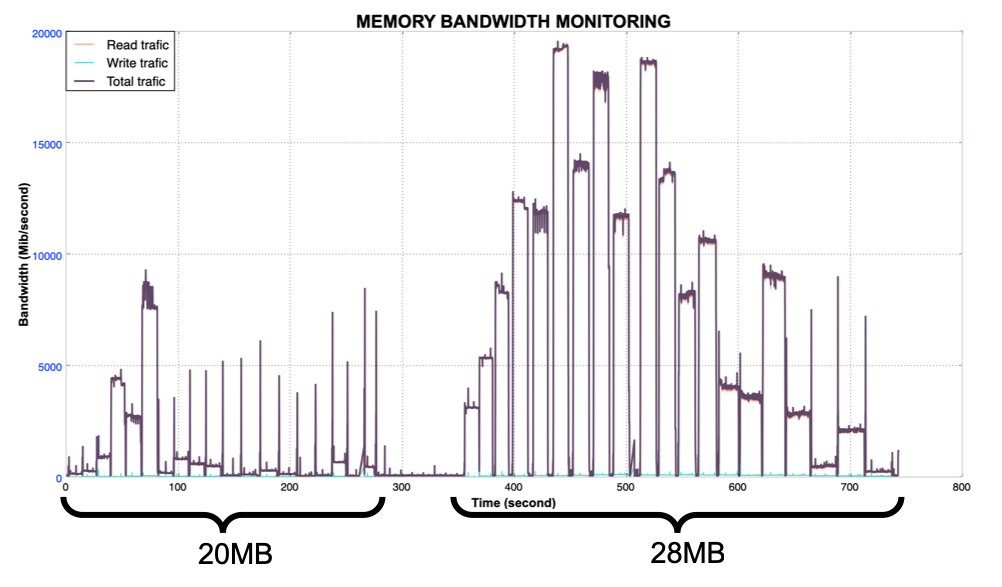
\includegraphics[width=14cm]{images/dml_bw_cacheL3.png}
        \caption{\label{pic:dml_bw_cacheL3} Évolution du traffic mémoire pour deux jeux de données de 20 et 28 MiB. Chaque jeu est accédé par 1 à 20 coeurs.}
        \end{figure}
        
        

    \subsubsection{Memory prefetcher}
    %%%%%%%%%%%%%%%%
        
        Dans l'expérimentation précédente nous montrons que le \textit{memory prefetcher} permet de maintenir le bonne performance du benchmark même lorsque des données sont évincées du cache. Dans cette partie nous questionnons l'utilité de son activation permanente. 
        
        Le benchmark \textit{DML\_MEM} a été utilisé pour réaliser des accès à un jeu de donnée dépassant la taille du plus grand niveau de cache. La \autoref{pic:dml_prefetch} montre la bande passante mémoire atteignable par un seul coeur lorsque le pré-chargement est activé ou non. On remarque que les performances sont similaires sauf pour une \textit{stride} de 64 bytes, correspondant à la taille d'une ligne de cache. Pour une telle \textit{stride}, la bande passante mémoire atteinte est réduite de 40\% lorsque le pré-chargement est désactivé.
        La raison de cette baisse vient d'un mécanisme couramment utilisé dans les architecture appelé le pré-chargement adjacent. Lors d'un accès mémoire, celui ci anticipe les futurs accès en chargeant aussi la ligne de cache suivante. Les codes parcourent souvent la mémoire de façon contiguë (données d'un tableau, instruction d'un programme). Avec l'utilisation d'une \textit{stride} de 128 bytes, nous montrons que le mécanisme de pré-chargement n'améliore plus les performances, car il ne s'occupe de charger que la ligne de caches adjacente (inutilisée). En désactivant le pré-chargement adjacent les performances sont même supérieures, car le bus mémoire n'est pas affecté par le transport de lignes de cache inutiles.
        
        \begin{figure}
        \center
        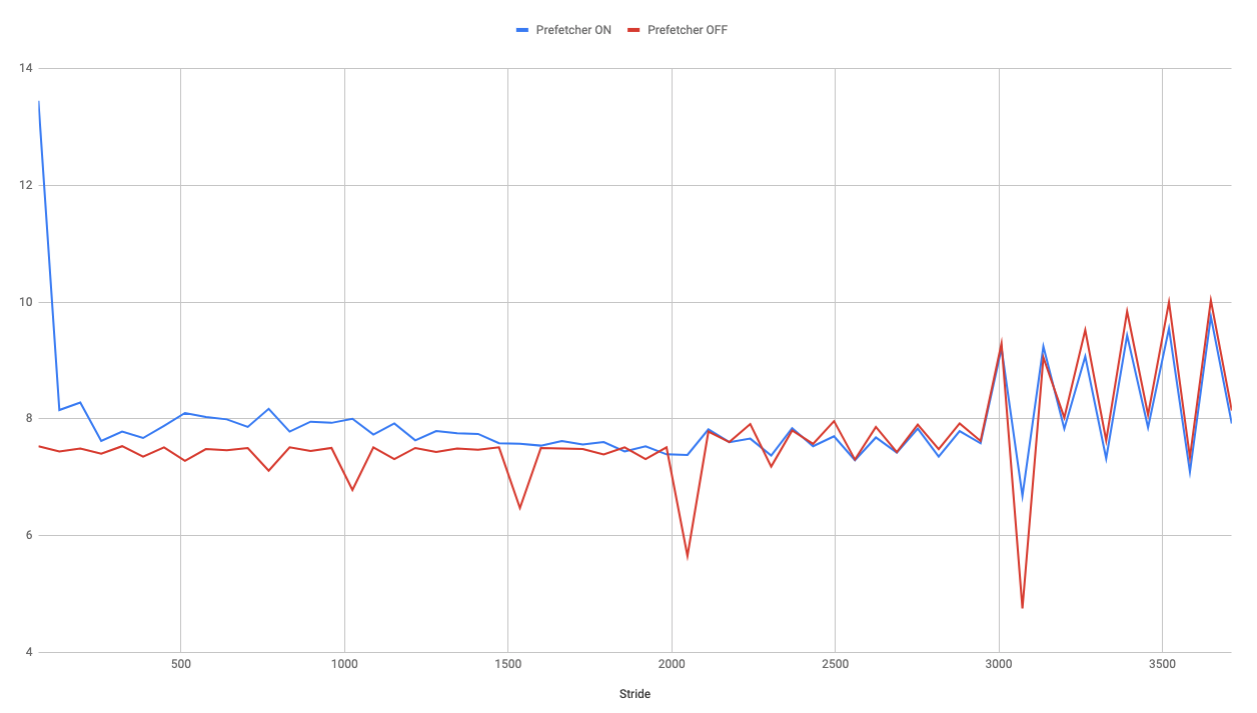
\includegraphics[width=10cm]{images/dml_prefetch.png}
        \caption{\label{pic:dml_prefetch} Performance mémoire d'un coeur lors de l'activation ou non du pré-chargement mémoire. }
        \end{figure}
         
        Pour montrer que l'activation du pré-chargement peut altérer les performances d'une application, la version parallèle du benchamrk \textit{DML\_MEM} a été utilisée. En effet, le pré-chargement de la ligne de cache adjacente n'est bénéfique que si elle est ensuite utilisée. Lorsqu'un seul coeur est actif, le chargement de cette ligne de cache n'impacte pas la performance du benchmark car le bus est loin d'être saturé (voir \autoref{pic:dml_prefetch}). La version parallèle de \textit{DML\_MEM} peut être utilisé pour charger la totalité des coeurs du processeur pour réaliser un accès mémoires toutes les deux lignes de cache (\textit{stride} 128 bytes). La désactivation du pré-chargement permet d'atteindre des performances 16\% supérieures (91 GB/s contre 73 GB/s lorsque le pré-chargement est actif). Ce type d'accès plus grand que deux lignes de cache est très courant dans les applications. Il peut donc être avantageux de le désactiver le pré-chargement de la ligne de cache adjacente pour ces portions de codes. De plus, le pré-chargement de données peut être réalisé manuellement grâce à des instructions telle que \verb| __builtin_prefetch (&a[i+j]); |.

        Si une architecture possède un \textit{prefetcher} défaillant, il peut être intéressant de vérifier si les coeurs du processeur sont capable de générer suffisamment de requête mémoire pour saturer le bus. En utilisant la version \textit{MPI} du benchmark, nous avons mesuré la performance du benchmark avec le mécanisme de pré-chargement adjacent actif ou non, avec différent nombre de coeurs. La \autoref{pic:dml_prefetch_mpi} montre que si le pré-chargement adjacent est désactivé la totalité des coeurs ne suffisent pas à saturer le bus mémoire. 
        
        
        \begin{figure}
        \center
        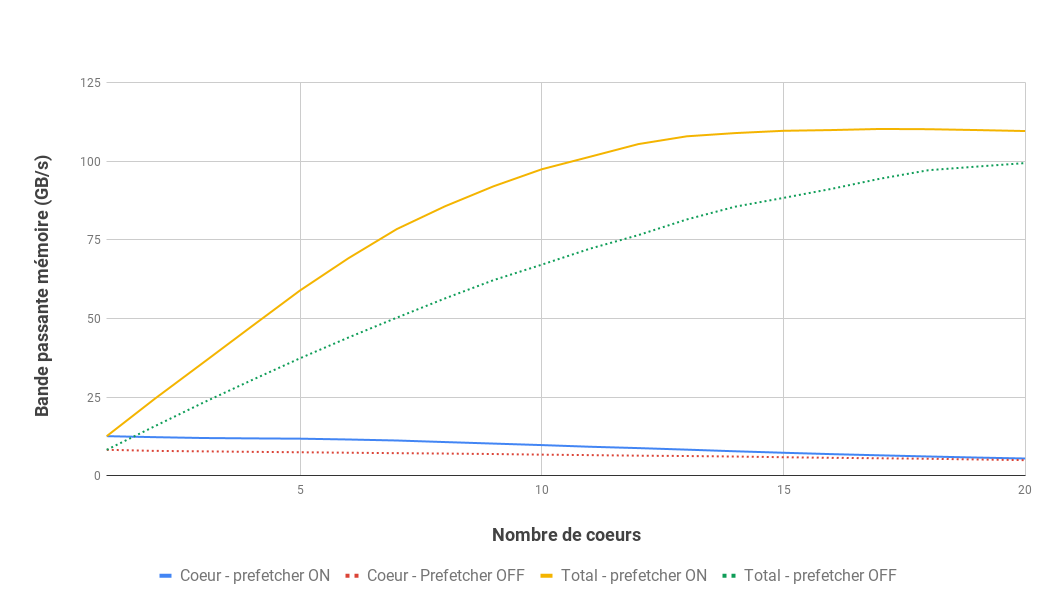
\includegraphics[width=14cm]{images/dml_prefetch_mpi.png}
        \caption{\label{pic:dml_prefetch_mpi} Performance du benchmark pour un jeu de données de 300 MiB avec un et plusieurs coeurs actifs lorsque le pré-chargement adjacent activé ou non.}
        \end{figure}
        
        
        
    
    \subsubsection{Déroulement de boucle} \label{sec:dml_unroll}
    %%%%%%%%%%%%%%%%
    Pour améliorer les performances du benchmark \textit{DML\_MEM}, l'optimisation du déroulement de boucle à été utilisée. Au vue de l'amélioration des performances obtenues, cette section présente comment l'optimisation est implémentée et comment les applications peuvent en tirer partie. 
    Le déroulement de boucle est une optimisation permettant de réduire l'impact de code permettant le contrôle de la boucle (test, incrémentation). Le principe est de développer manuellement le code de plusieurs itérations dans la boucle et d'incrémenter ensuite la boucle de même nombre de déroulement. Ainsi, la proportion de code responsable du contrôle de la boucle est réduite par rapport à l'intérieur de la boucle. Une première version du code utilisé pour réaliser le déroulement est présenté dans l'\autoref{lst:dml_unroll_orig}. Pour permettre au processeur commencer les accès mémoire grâce au mécanisme d'exécution dans le désordre, 4 pointeurs différents sont utilisés. Chaque pointeur pointe vers une stride et la valeur est sommée dans la variable \verb|sum|. Les résultats obtenus par cette première version sont mauvaises, notamment pour des jeux de données situés dans les premiers niveaux de cache (baisse de la performance d'un facteur trois). Cette effondrement de performance vient de l'incapacité du compilateur à appliquer sa propre optimisation de déroulement de boucle. Cette première version étant plus mauvaise, la performance est fortement dégradée. Par ce premier résultat, nous souhaitons attirer l'attention du programmeur sur le fait que le compilateur réalise déjà certaines optimisations. Il peut être contre-productif de la réaliser soit même. 
    
    \begin{lstlisting}[label=lst:dml_unroll_orig ,language=C, caption=Première version du déroulement de la boucle par 4.]
for (rep = 0; rep < repeat; rep++) {
    DML_DATA_TYPE *p1 = mat;
    DML_DATA_TYPE *p2 = p1 + step;
    DML_DATA_TYPE *p3 = p2 + step;
    DML_DATA_TYPE *p4 = p3 + step;
    for (steps = 0; steps < ops_per_scan; steps++) {
        sum += *p1;
        p1 += xstep;
        sum += *p2;
        p2 += xstep;
        sum += *p3;
        p3 += xstep;
        sum += *p4;
        p4 += xstep;
    }
}
\end{lstlisting}


    L'erreur dans la première version du déroulement est l'utilisation d'une unique variable de sommation. En effet, cette unique variable qui doit être incrémentée à chaque lecture d'une stride créée une dépendance empéchant le code d'exécuter deux opérations d'addition par cycle. L'\autoref{lst:dml_unroll_spe} présente la version \textit{special} de l'optimisation du déroulement qui utilise autant de variables de sommation que de déroulements réalisés. Avec cette version, la performance du benchmark dans les caches L1 et L2 est améliorer respectivement de 12\% et 30\%. 
    
    \begin{lstlisting}[label=lst:dml_unroll_spe ,language=C, caption=Deuxième version du déroulement par 4 utilisant 4 variables sum.]
for (rep = 0; rep < repeat; rep++) {
    BM_DATA_TYPE *p1 = mat;
    BM_DATA_TYPE *p2 = p1 + step;
    BM_DATA_TYPE *p3 = p2 + step;
    BM_DATA_TYPE *p4 = p3 + step;
    for (steps = 0; steps < ops_per_scan; steps++) {
        sum1 += *p1;
        p1 += xstep;
        sum2 += *p2;
        p2 += xstep;
        sum3 += *p3;
        p3 += xstep;
        sum4 += *p4;
        p4 += xstep;
    }
}
return sum1 + sum2 + sum3 + sum4;
\end{lstlisting}
    
    La suite de cette expérimentation s'intéresse au nombre de déroulement de la boucle et de son impacte sur la performance de benchmark. Pour cela, le benchmark a été exécuté en utilisant entre 1 et 64 déroulements sur un jeu de données remplissant 80\% du cache de niveau 2. Les résultats obtenus sont présentés dans le \autoref{tab:dml_unroll_bench}. Nous vérifions que l'optimisation du déroulement est bénéfique pour la performance du benchmark améliorant les performances progressivement de 117.8 GB/s à 337 GB/s pour un déroulement de boucle allant de 2 à 8 fois. On remarque que moins d'instructions sont exécutées et que le nombre d'instructions exécutées chaque cycle augmente de 2 à 3.22. Au delà de 8 déroulements, la performance du benchmark se dégrade progressivement. Avec 64 déroulements de la boucle, le nombre d'instructions exécutées double et les performance s'effondre à 140 GB/s. De nouveau, nous montrons ici que la mesure du nombre d'instructions exécutées chaque cycle n'est pas un bon indicateur pour évaluer la performance d'un code. 
    

    \begin{table}[h!]
    \centering
    \begin{tabular}{|c|c|c|c|}
    \hline
    \rowcolor[HTML]{EFEFEF} 
    \multicolumn{1}{|l|}{\cellcolor[HTML]{EFEFEF}Nb. de déroulements} & \multicolumn{1}{l|}{\cellcolor[HTML]{EFEFEF}Bande passante (GB/s)} & \multicolumn{1}{l|}{\cellcolor[HTML]{EFEFEF}Nb. d'instructions exécutée} & \multicolumn{1}{l|}{\cellcolor[HTML]{EFEFEF}Instruction par cycle} \\ \hline
    1 & 117.8 & 4204612342 & 2 \\ \hline
    2 & 235.47 & 3159994082 & 2.99 \\ \hline
    4 & 311.07 & 2634059908 & 3.28 \\ \hline
    8 & 337.96 & 2380891060 & 3.22 \\ \hline
    16 & 306.66 & 2483260088 & 3.07 \\ \hline
    32 & 315.17 & 2513084995 & 3.19 \\ \hline
    64 & 140.98 & 4993000253 & 2.87 \\ \hline
    \end{tabular}%
    \caption{Performance du benchmark \textit{DML\_MEM} utilisant plusieurs taille de déroulement de la boucle pour un jeu de donnée atteignant 80\% du cache L2.}
    \label{tab:dml_unroll_bench}
    \end{table}
    
    Pour comprendre la mauvaise performance du code lorsqu'il est déroulé plus de 8 fois, nous avons extrait leur code assembleur. L'\autoref{lst:unroll4} montre comment le code du benchmark est généré lorsque 4 déroulements sont réalisés. On remarque que les 4 opérations d'additions sont vectorisées et qu'elles se suivent dans le code permettant à l'exécution dans le désordre de les exécuter deux par deux. On remarque aussi que 16 des 32 registres \verb|%xmm| sont utilisés. L'\autoref{lst:unroll16} expose le code assembleur du benchmark déroulant 16 fois la boucle. Le processeur utilise alors la totalité des 32 registres \verb|%xmm|. Cependant, ce n'est pas suffisant pour réaliser tout les traitements et il est obligé de stocker et charger certains élements depuis la pile. L'exécution des operations d'additions vectorisées est alors ralentie. Pour comprendre l'effondrement des performances lors de 64 déroulements, l'analyse du code assembleur est une fois de plus précieuse. Lorsque 64 déroulements sont utilisés, le compilateur ne parvient plus à générer d'additions vectorielles. Les performances sont alors divisée par deux, alors que l'IPC est presque similaire. 
    

\begin{minipage}{.45\textwidth}
\begin{lstlisting}[
label=lst:unroll4,
basicstyle={\scriptsize\ttfamily},
identifierstyle={\color{black}},
language={[x86masm]Assembler},
tabsize=2,
numbersep=8pt,
frame=tlbr,framesep=2pt,framerule=0pt,
morekeywords ={class,run},
caption=Boucle déroulée 4 fois.
]
vmovhpd (%r14,%r11,8),%xmm8,%xmm9
lea     (%rsi,%r12,8),%r14
vmovhpd (%r15,%r11,8),%xmm10,%xmm11
lea     (%r12,%r11,2),%r12
vmovsd  (%r15),%xmm14
vmovhpd (%r14,%r11,8),%xmm12,%xmm13
vmovhpd (%r15,%r11,8),%xmm14,%xmm15
vaddpd  %xmm9,%xmm3,%xmm3
vaddpd  %xmm11,%xmm2,%xmm2
vaddpd  %xmm13,%xmm1,%xmm1
vaddpd  %xmm15,%xmm0,%xmm0
\end{lstlisting}
\end{minipage}%%
\hfill
%&
%
\begin{minipage}{.45\textwidth}
\begin{lstlisting}[
label=lst:unroll16,
basicstyle={\scriptsize\ttfamily},
identifierstyle={\color{black}},
tabsize=2,
language={[x86masm]Assembler},
numbersep=8pt,
xleftmargin=0.5cm,frame=tlbr,framesep=2pt,framerule=0pt,
morekeywords ={class,run},
caption=Boucle déroulée 16 fois.
]
vmovsd  (%r15),%xmm30
vmovhpd (%r15,%r9,8),%xmm30,%xmm30
lea     (%r14,%rdx,8),%r15
vaddpd  %xmm30,%xmm31,%xmm31
vmovsd  (%r15),%xmm30
vmovhpd (%r15,%r9,8),%xmm30,%xmm30
lea     (%r11,%rdx,8),%r15
vaddpd  %xmm30,%xmm3,%xmm3
. 
. 
. 
\end{lstlisting}
\end{minipage}
    
    
    Pour mieux apprécier les performances de chaque déroulement, le benchmark est exécuté dans les différents niveaux de la hiérarchie mémoire. Les résultats sont présentés sur le graphique de la \autoref{pic:dml_unroll_best}. Dans le cache L1, l'utilisation 4 et 8 pointeurs permet d'améliorer la performance de 40 GB/s. On remarquera aussi la mauvaise performance de deux déroulements de la boucle dans ces premiers niveaux de caches. Cette expérimentation permet de montrer que la manière optimale d'accéder à un jeu de données présent dans les caches est d'utiliser entre 8 et 16 pointeurs différents. Au delà, le nombre de restreint de registres disponibles pour le processeur détériore la performance. La performance dans les caches des versions avec 4, 8 ou 16 déroulements est supérieur à celle du compiltateur \verb|ICC| (déroulement de 1). Lorsque les données sont dans la mémoire, le déroulement n'améliore pas les performances. 

    \begin{figure}
    \center
    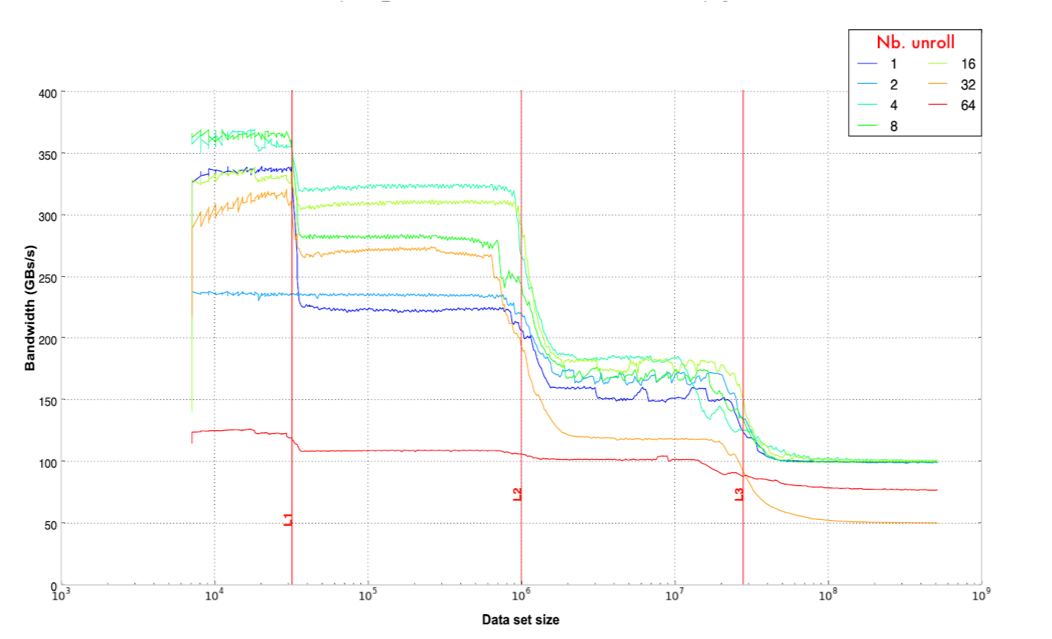
\includegraphics[width=16cm]{images/dml_unroll_best.png}
    \caption{\label{pic:dml_unroll_best} Performance de plusieurs déroulements pour une stride de 8 bytes (lecture de tous les éléments).}
    \end{figure}
    
    
    \subsubsection{Large page} \label{sec:dml_large_page}
    %%%%%%%%%%%%%%%%

    L'expérimentation suivante à pour objectif de comparer la performance du benchmark lors de l'utilisation de différentes tailles de pages mémoire. Comme présenté dans la \autoref{sec:page}, l'utilisation de page de plus grande taille permet d'améliorer la performance du système mémoire, notamment en accélérant le traitement de la TLB. Les pages plus larges permettent aussi de réduire les conflits d'associativité dans les caches. L'expérimentation réalisée avec un coeur actif a permis d'obtenir les résultats présentés dans le \autoref{tab:large_page_memory}. La performance des caches est améliorée avec l'utilisation des pages larges, jusqu'à 30\% dans le cache L3. Lorsque le jeu de donnée est dans le L3, la mesure du nombre d'évenements \textit{miss} de la TLB augmente d'un facteur 300. Cependant, la TLB arrive à masquer la majorité de ces \textit{miss} et conserve une bonne performance (150 GB/s).

    \begin{table}[]
    \centering
    \resizebox{\textwidth}{!}{%
    \begin{tabular}{l|c|c|c|c|c|}
    \cline{2-6}
     & \cellcolor[HTML]{EFEFEF}L1 (GB/s) & \cellcolor[HTML]{EFEFEF}L2 (GB/s) & \cellcolor[HTML]{EFEFEF}L3 (GB/s) & \cellcolor[HTML]{EFEFEF}Memoire (GB/s) & \cellcolor[HTML]{EFEFEF}dTLB-load-misses \\ \hline
    \multicolumn{1}{|l|}{\cellcolor[HTML]{EFEFEF}Page de 4 KiB} & 320 & 220 & 150 & 13.40 & 2254025 \\ \hline
    \multicolumn{1}{|l|}{\cellcolor[HTML]{EFEFEF}Page de 2 MiB} & 340 & 225 & 200 & 13.45 & 6556 \\ \hline
    \end{tabular}%
    }
    \caption{Performance du benchmark \textit{DML\_MEM} utilisant deux tailles de pages. La performance dans les 4 niveaux de la hiérarchie mémoire a été mesurée avec le benchmark et le nombre d'évènements \textit{miss} lorsque le jeu de donnée est dans le cache L3.}
    \label{tab:large_page_memory}
    \end{table}
    
    
    Nous nous sommes ensuite intéressé aux performances du benchmark lorsque plusieurs coeurs sont actifs, avec et sans l'utilisation des pages larges. Nous observons les mêmes écarts de performances lorsque le jeu de données est stocké dans les caches. Lors de l'utilisation de pages standards (4 KiB), nous constatons que lorsque la taille du jeu de données approche de la taille des jeux de données, la performance commence à se détériorer. Avec l'utilisation des pages de 4 MiB, la performance dans chaque niveau de cache est constante et ne se détériore que lorsque le jeu de donnée dépasse la taille du niveau de cache. Cette effet observé lors de l'utilisation de petites pages est appelé \textit{page coloring} \cite{Zhang2009}.
  
    \begin{figure}
    \center
    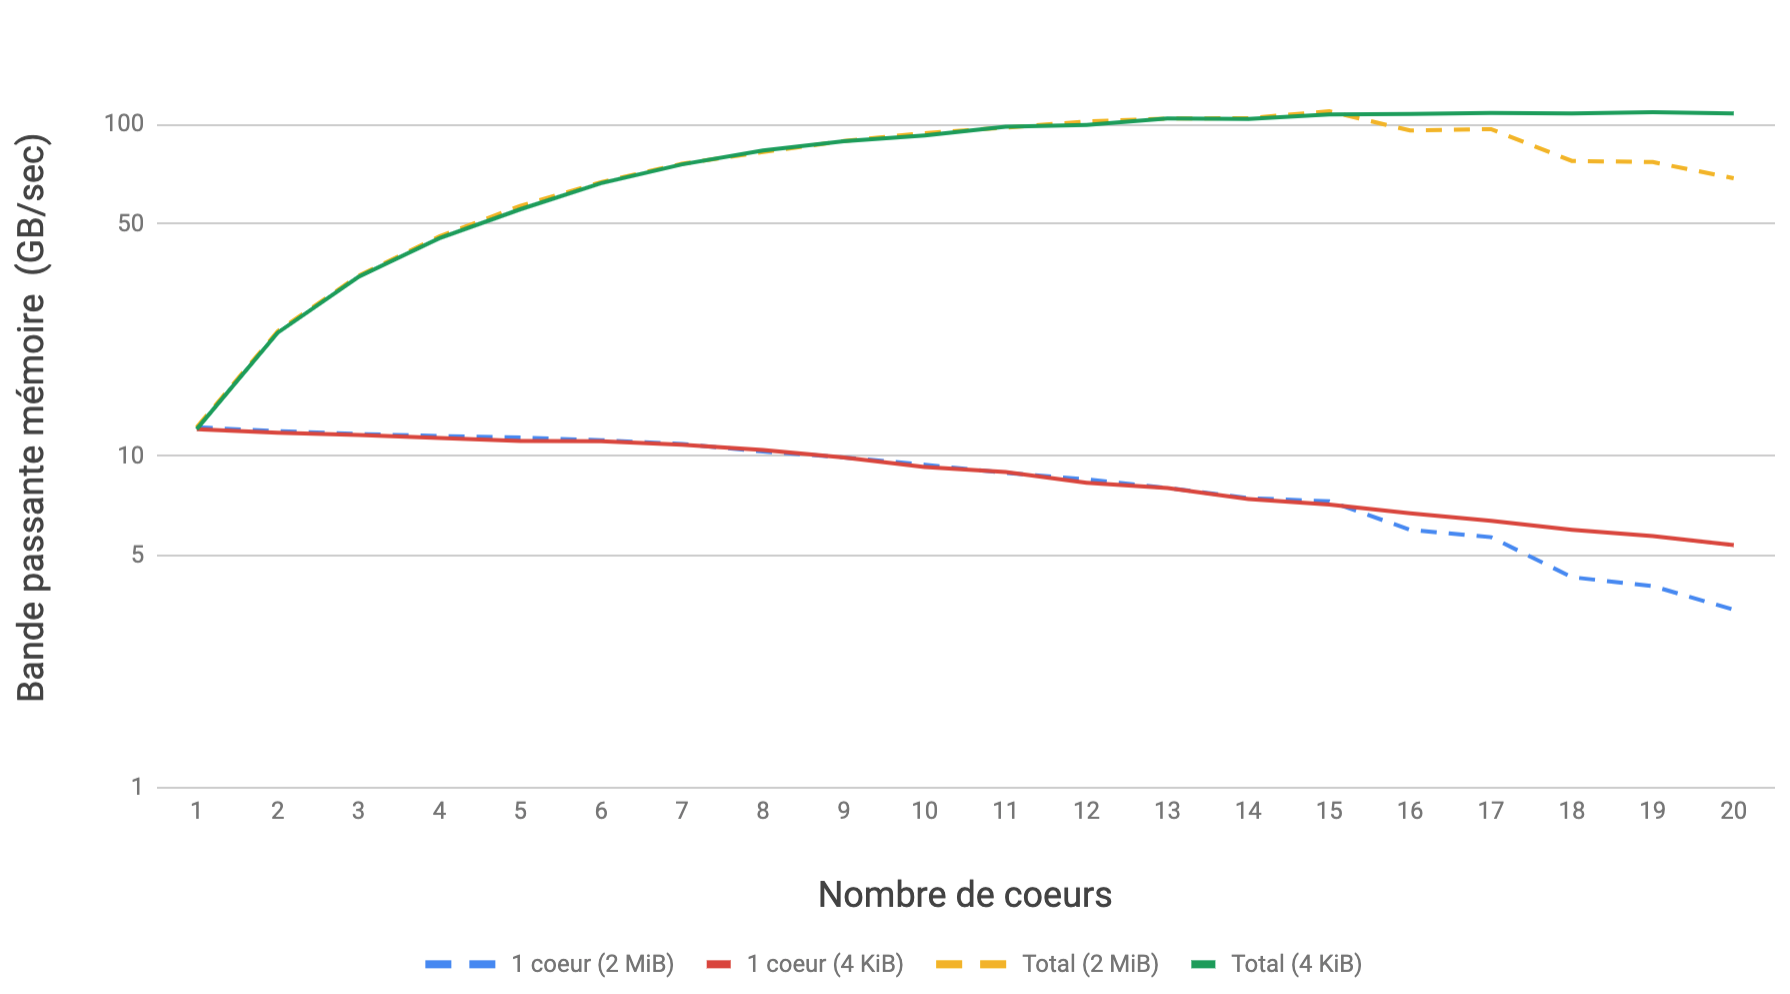
\includegraphics[width=14cm]{images/dml_large_page_bw.png}
    \caption{\label{pic:dml_large_page_bw} Bande passante mémoire par coeur et pour plusieurs coeurs utilisant deux tailles de pages pour stocker un jeu de données de 2 GiB.}
    \end{figure}
    
    Le graphique de la \autoref{pic:dml_large_page_bw} montre les performances du benchmark avec un ou plusieurs coeurs actifs sur un jeu de donnée de 2 GiB. Nous remarquons que la performance du benchmark baisse lorsque au moins 15 coeurs sont utilisés avec des pages large. La performance par coeur diminue de 5.39 GB/s à 3.44 GB/s. Nous n'avons pour le moment pas réussi à expliquer ce problème qui affecte tout les jeux de données supérieurs à 2 GiB.
    
    Bien que la TLB limite rarement les performances des applications réelles, le recours à l'utilisation de pages larges peut être bénéfique. Les version récentes du noyeau Linux peuvent choisir elles mêmes lors de l'allocation mémoire si le recours à des pages plus grandes peut être bénéfique pour l'application (Red Hat Transparent Huge Pages (THP)). Comme nous montrons dans cette dernière expériences que l'utilisation de page de 2 MiB peuvent détériorer les performances, il est conseillé que cette responsabilité reviennent à l'utilisateur qui devra décider ou non de leur utilisation en fonction de son application. 
  


    
    \subsubsection{Fréquence et coeurs: impact sur la bande passante} \label{sec:dml_core_vs_freq}
    %%%%%%%%%%%%%%%%
    
    Dans cette expérimentation nous avons mesurer la bande passante mémoire atteignable par notre benchmark pour différentes configuration de fréquence et nombre de coeurs actifs. Les résultats sont visibles sur la \autoref{pic:dml_core_vs_freq}. Comme dans l'expérimentation précédente (\autoref{sec:dml_saturation}), nous démontrons que la totalité des coeurs n'est pas nécessaire pour saturer la bande passante. Cette expérience montre aussi que les coeurs utilisés n'ont pas besoin d'utiliser leur fréquence maximale. En effet, notre benchmark sature le bus mémoire avec 17 coeurs cadencés à seulement 2.1 GHz. Le script utilisé pour générer la \autoref{pic:dml_core_vs_freq} annote automatique le graphique pour identifier rapidement les maximums. Une telle utilisation du benchmark \textit{DML\_MEM} permet d'identifier le couple  \verb|{fréquence, nombre de coeurs}| minimale pour saturer le bus mémoire. Pour des applications limités par la performance de ce dernier, il peut être intéressant de désactiver les coeurs supplémentaire ou de plafonner la fréquence du processeur pour limiter la consommation électrique. En plus de vérifier la présence potentielle de bogues dans l'architecture, cette expérimentation peut permettre à un utilisateur de choisir la meilleur configuration pour un achat de nouveaux processeurs. 
    
    \begin{figure}
    \center
    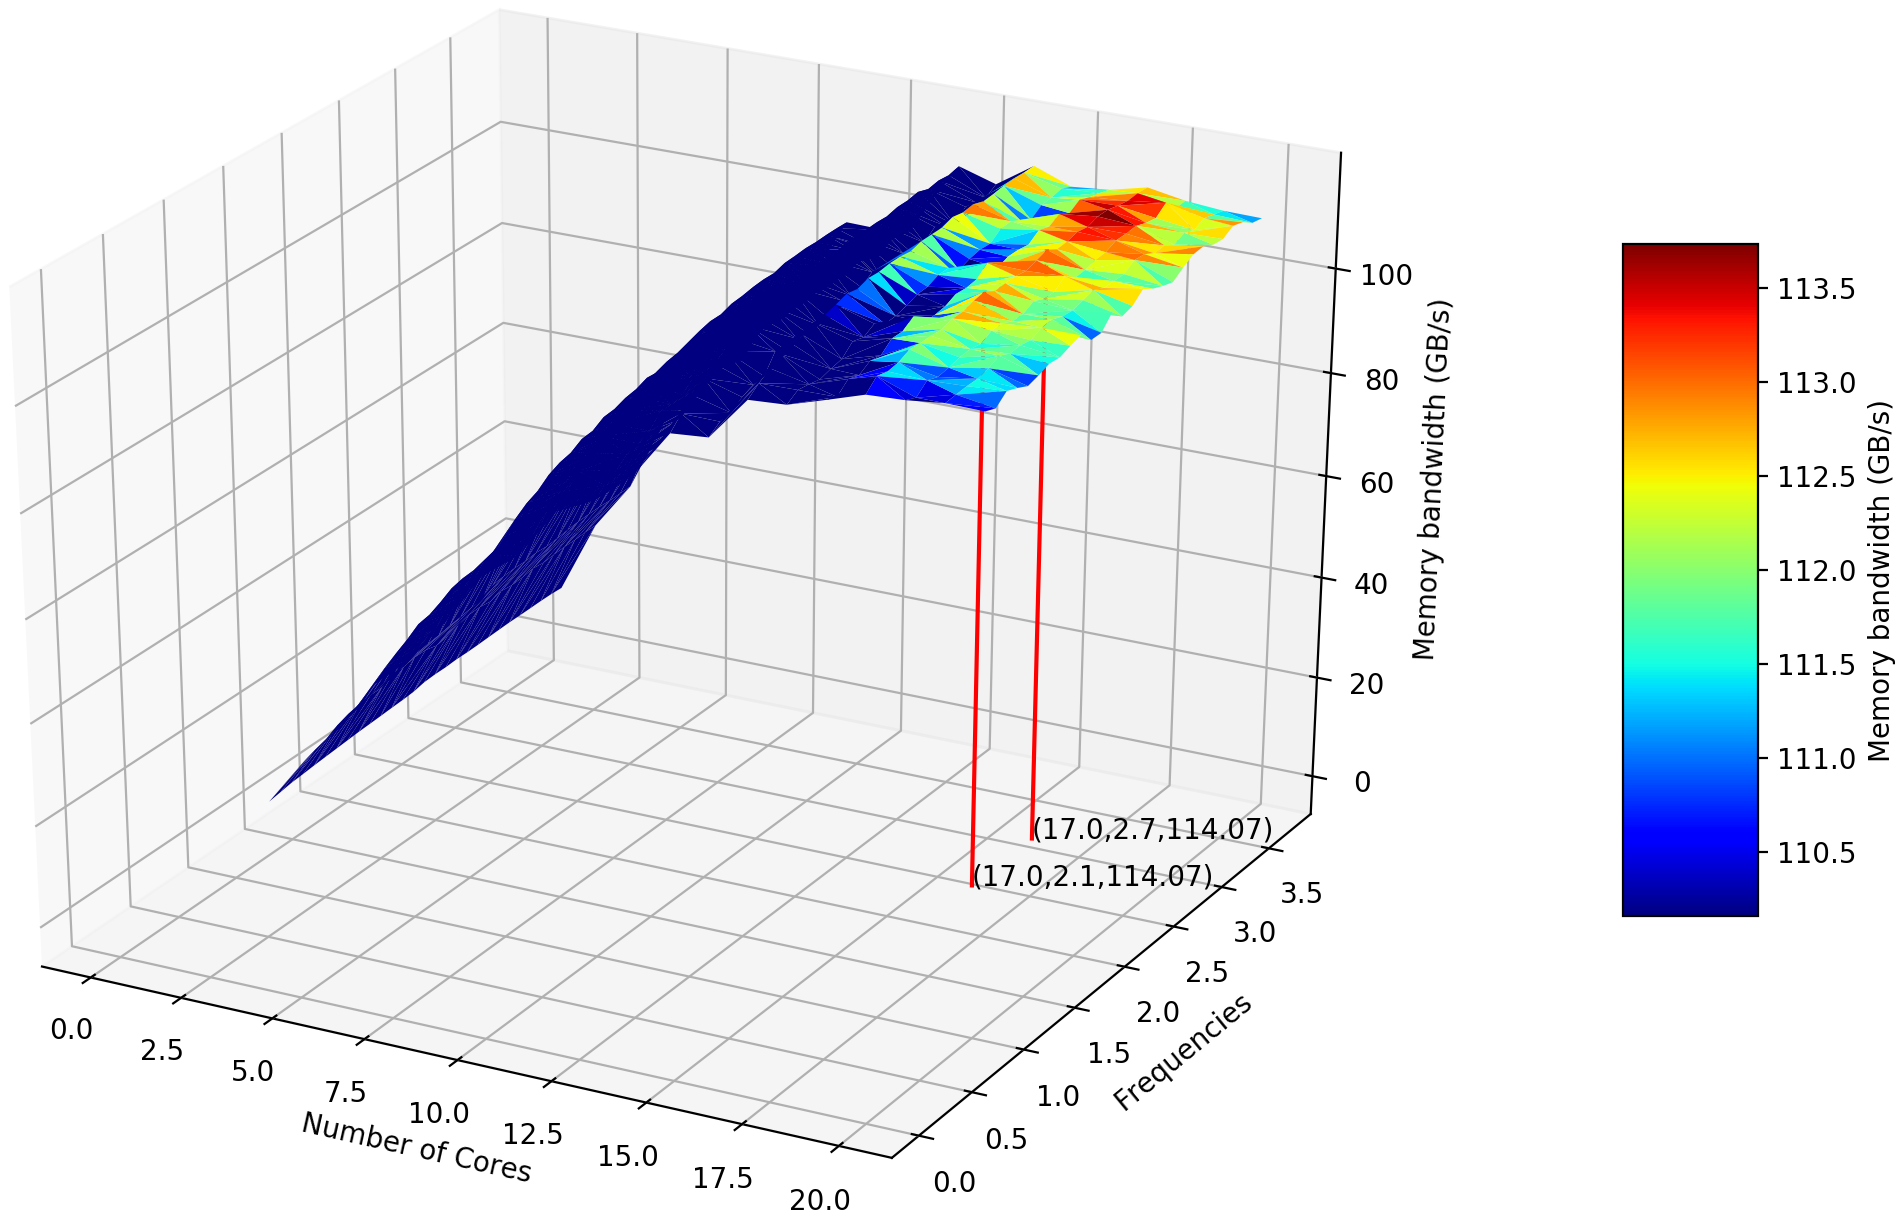
\includegraphics[width=14cm]{images/dml_core_vs_freq.png}
    \caption{\label{pic:dml_core_vs_freq} Mesure de la performance du bus mémoire lors de lors de l'utilisation de différent nombre de coeurs plafonnés à différentes fréquences}
    \end{figure}
    


    
    

\subsection{Conclusion}
%%%%%%%%%%%%%%%%%%%%%%%%%%%%%%%%%%%%%%%%%%%%%%%%%%%%%%

    Cette section s'intéresse au \textit{DML\_MEM}, un benchmark permettant de caractériser de multiples parties du système mémoire. Le benchmark permet de réaliser des accès mémoire grâce à des motifs de strides pour caractériser les plateformes pour des codes de types \textit{stencil}.
    Nous montrons que la micro-architecture peut avoir des comportements très inattendus lors de l'utilisation de certaines tailles de saut. A travers ces expérimentations nous souhaitons attirer l'attention du programmeur sur la complexité de la micro-architecture et de la nécessité de sa caractérisation.
    Lors des travaux de thèse, l'utilisation de cet outil nous a permis de caractériser plusieurs plateformes différentes et de déceler des bugs majeurs dans certaines d'entre elles. Les accès par stride mettent la pression sur le pré-chargeur mémoire, l'utilisation de cet outil peut alors être aussi intéressant lors de la conception d'une nouvelle architecture que lors de sa caractérisation pour le portable d'une application réelle. 
\newpage

\newpage
\section{Benchmark d'unité arithmétique}\label{sec:kg}



\subsection{Introduction}
%%%%%%%%%%%%%%%%%%%%%%%%%%%%%%%%%%%%%%%%%%%%%%%%%%%%%
   
     
    La principale opportunité pour construire un supercalculateur exaflopique va être l'utilisation d'architectures hétérogènes. Ceci sera possible notamment grâce à Gen-Z. De nouveaux accélérateurs différents de ceux que nous connaissons vont être disponibles. La nécessité de les caractériser est à l'origine de ce premier outil.

    \subsubsection{Motivations}
    
    Les applications HPC exécutent, pour la grande majorité, des instructions sur des nombres à virgule. L'exécution de ces opérations dites \textit{flottantes} est réalisée par un composant appelé unité de calcul en virgule flottante (FPU). La performance des applications est donc dépendante de celle de ces accélérateurs. La performance de la majorité des applications est limitée par la performance du système mémoire et les efforts de développement se sont en grande partie consacrés à la caractérisation de cette partie de l’architecture. Cependant, avec ces nouvelles architectures, la différence de performance entre les unités de calculs et celle du système mémoire devrait être plus équilibrée. Il est donc important d'avoir les outils nécessaires pour les caractériser.
    Bien que le comportement des FPU des architectures actuelles soit connu,  certaines particularités soient encore difficiles à caractériser (exécution dans le désordre, dépendances entre instructions, fréquence atteignable pour un type d'instruction vectorielle). 
    Il est nécessaire de connaître la performance maximale d'un processeur (mesurée en FLOP) pour différents types de calculs. Celle-ci peut alors être utilisée pour apprécier les performances d'un code grâce à des modèles de type Roof line (voir \autoref{sec:roofline}). Pour obtenir cette performance maximale, certaines techniques utilisent les caractéristiques matérielles pour la calculer. Cependant, la complexité des architectures nous a souvent montré que la performance réellement atteignable pouvait être différente (inférieur, mais aussi supérieur). En utilisant un benchmark, il est aussi possible de trouver des comportements cachés de l'architecture ou d'en déceler des bogues. 
    Le benchmark présenté utilise le langage assembleur. Ce choix a été motivé par la volonté de s'assurer que les instructions générées été bien exécuté. En effet, les compilateurs deviennent toujours plus performants et optimisent les codes rendant l'analyse de performance plus difficile. De plus, ils peuvent comprendre l'artificialité d'un code et contourner son exécution. En générant nous même le code assembleur, nous nous assurons que la performance du code mesurée est bien celle attendue.
    


   
    
    
    
    \subsubsection{Floating Point Unit (FPU)}
    %%%%%%%%%%%%%
        La FPU est un composant majeur des ordinateurs et a connu de nombreuses évolutions au fil des générations. À l'origine, les FPU étaient des composants additionnels pouvant être ajoutés sur la carte mère pour accélérer l'exécution de calcul en virgule flottante (\autoref{pic_cpu_fpu}\footnote{\url{https://en.wikipedia.org/wiki/Floating-point_unit}}). C'est pour cela qu'il est commun de designer ce composant comme un accélérateur. Cependant, les applications réalisant de plus en plus de calculs de ce type, les FPU ont ensuite été directement intégrées au processeur (\autoref{pic_cpu_fpu_recent}\footnote{\url{https://www.extremetech.com/computing/263963-intel-reverses-declares-skylake-x-cpus-two-avx-512-units}}). Ceci a notamment permis de réduire les latences. De plus, avec l'apparition de plates-formes multiprocesseurs, la gestion d'erreurs et d'exception liées aux FPU était devenue très difficile. Le premier processeur Intel à posséder une FPU et un CPU sur la même puce est le processeur Intel 80486DX produit en 1989.

        Aujourd'hui, les FPU sont des composants de haute performance permettant d'exécuter des calculs sur des nombres réels grâce à des instructions vectorielles. La FPU reçoit ses instructions du même décodeur que celui de l'unité de calcul pour les nombres entiers (ALU). Lorsque les premiers étages du pipeline (voir \autoref{sec:pipeline}) ont décodé l'instruction à exécuter, le séquenceur choisi si elle doit être exécutée l'ALU ou la FPU. 
        Les FPU sont un des composants les plus importants de l'architecture. Les applications de HPC réalisent beaucoup de calculs sur nombre flottants qui sont exécutés par les unités de calcul flottant. Ces unités sont beaucoup sollicitées et il est important d'en connaître les caractéristiques: débit, latence, fréquence maximale soutenable par le processeur. En effet, les instructions vectorielles les plus longues utilisent plus de transistors pour être utilisées. Ainsi, la chaleur émise par le processeur varie et généralement les instructions les plus longues ne peuvent être exécutées aux fréquences maximales du processeur. Les différentes fréquences atteignables pour un type d'instruction peuvent être difficiles à prévoir.
        Les modèles tels que celui du \textit{roof line} (voir \autoref{sec:roofline}), ont besoin de ces caractéristiques pour pouvoir comparer la performance mesurée d'une application à celle théoriquement atteignable. 
        

        

        \begin{figure}
            \centering
            \begin{subfigure}[b]{0.45\linewidth}
                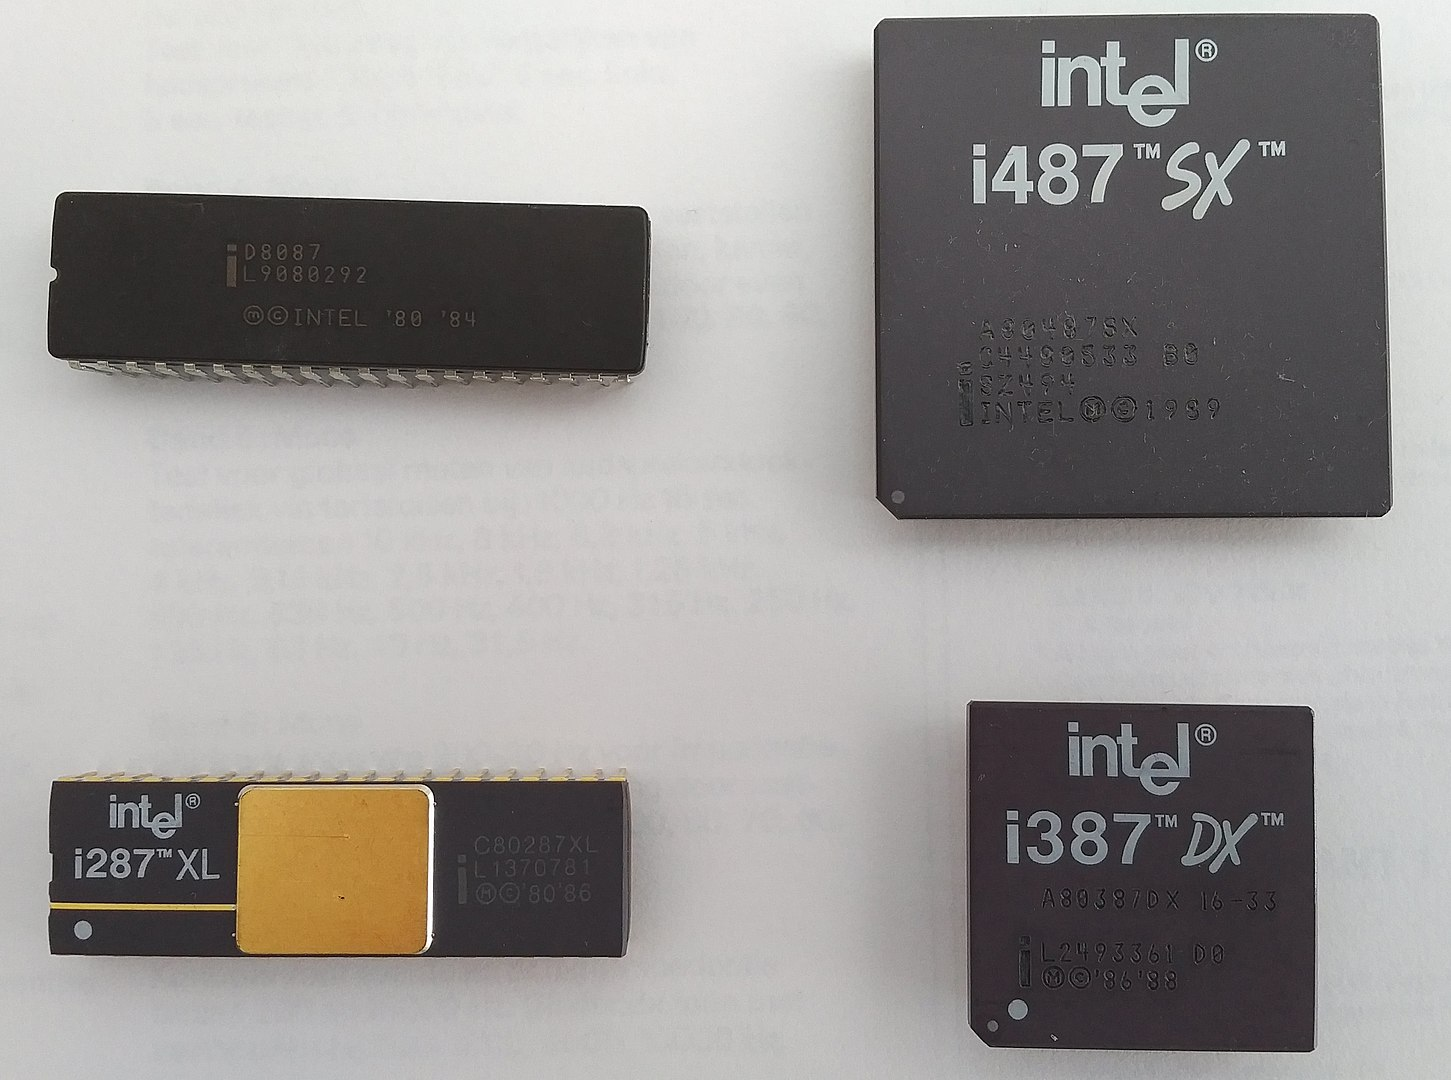
\includegraphics[width=\linewidth]{images/cpu_fpu.jpg}
                \caption{Différentes FPU qui pouvaient être achetées séparément des processeurs.}
                \label{pic_cpu_fpu}
            \end{subfigure}
            ~ %add desired spacing between images, e. g. ~, \quad, \qquad, \hfill etc. 
              %(or a blank line to force the subfigure onto a new line)
            \begin{subfigure}[b]{0.45\linewidth}
                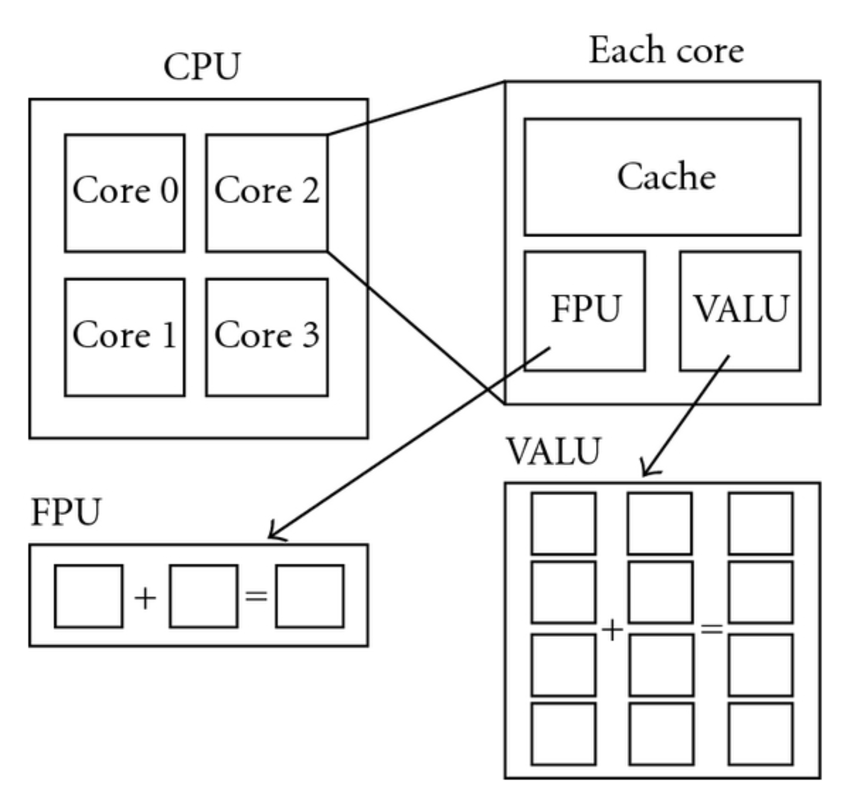
\includegraphics[width=\linewidth]{images/cpu_fpu_recent.png}
                \caption{Aujourd'hui la FPU est positionnée directement sur chaque coeur du processeur.}
                \label{pic_cpu_fpu_recent}
            \end{subfigure}
            \caption{La FPU d'un processeur est un co-processeur permettant d'exécuter efficacement des instructions de calculs arithmétiques. }\label{fig:cacheinclusionpolicy}
        \end{figure}
        
       
 
        

    
    \subsubsection{Objectifs}
    %%%%%%%%%%%%%
    
        L'objectif principal de cet outil est de caractériser finement les performances des unités de calcul en virgule flottante (FPU).
        La première caractéristique pouvant être mesurée est la performance maximale atteignable par la FPU pour un certain type d'instruction. Cette performance est mesurée en $FLOPS$ et peut être mesuré pour des types et des tailles d'instructions différents. L'avantage de cette unité est de rendre les résultats du Kernel Generator comparable avec ceux d'autre benchmark (tel que \textit{HPL}). 
        La deuxième caractéristique mesurable est la latence des instructions. Il peut être intéressant de connaître celle-ci lors de l'exécution d'instructions dépendantes.
        D'autres comportements doivent être caractérisés pour anticiper la performance de certaines applications. Parmi eux, celui de l'unité d'exécution dans le désordre. Certains codes comportant beaucoup de dépendances sont limités par la faculté du processeur à exécuter plusieurs chaînes de dépendance.


        
\subsection{Kernel Generator}    
%%%%%%%%%%%%%%%%%%%%%%%%%%%%%%%%%%%%%%%%%%%%%%%%%%%%%

        Nous proposons un outil permettant de générer des kernels de calculs en assembleur pour caractériser finement le comportement des FPU. Pour expliquer son comportement, ce chapitre utilise principalement des processeurs Intel Xeon Skylake, mais le but de l'outil est d'être utilisé pour caractériser des microarchitectures différentes. 
        L'outil proposé est un générateur de benchmarks qui permet de trouver la performance crête d'un processeur pour un certain type d'instruction vectorielle utilisant différentes configurations (type d'instructions, dépendances...).
        
        

    \subsubsection{Concept}
    %%%%%%%%%%%%%%%%%%%%%%

            L'outil \textit{Kernel Generator} a été construit pour répondre aux objectifs fixés dans la section précédente. Il permet de tester les caractéristiques de la FPU d'un processeur grâce à l'exécution d'un kernel écrit en assembleur comportant des instructions de calcul arithmétique. Les instructions utilisées peuvent être scalaires ou vectorielles. La version actuelle de l'outil supporte les instructions de types scalaire, SSE, AVX2 et AVX512. 
            Grâce à ses différentes options, l'utilisateur peut générer des kernels d'instructions de types et de taille différents. La valeur de l'outil vient de son utilisation et des différents tests que le programmeur veut réaliser. Le \textit{Kernel Generator} n'est pas un benchmark qu'il suffit d'exécuter pour obtenir des résultats. Cet outil respecte notre démarche initiale qui est de donner les outils à l'utilisateur pour l'aider dans son travail de profilage des applications et de caractérisation des architectures. 
            L'outil peut aussi être utilisé pour détecter des problèmes de la microarchitecture lors de l'exécution intensive d'instruction de calculs. Détecter ces comportements cachés peut ensuite permettre de mieux apprécier la performance d'une application réelle. 
        
     
        
            La \autoref{pic_kg_workflow} montre les étapes majeures de l'exécution du générateur de kernel. L'utilisateur exécute le générateur en utilisant les différentes options présentées dans la \autoref{sec:kg_option}. À partir des arguments le générateur écrit un programme en langage C++ qu'il compile et exécute. Les résultats sont ensuite présentés sous forme de texte dans le terminal ou sous forme de graphique (nécessite python). 
        
    
            \begin{figure}
            \center
            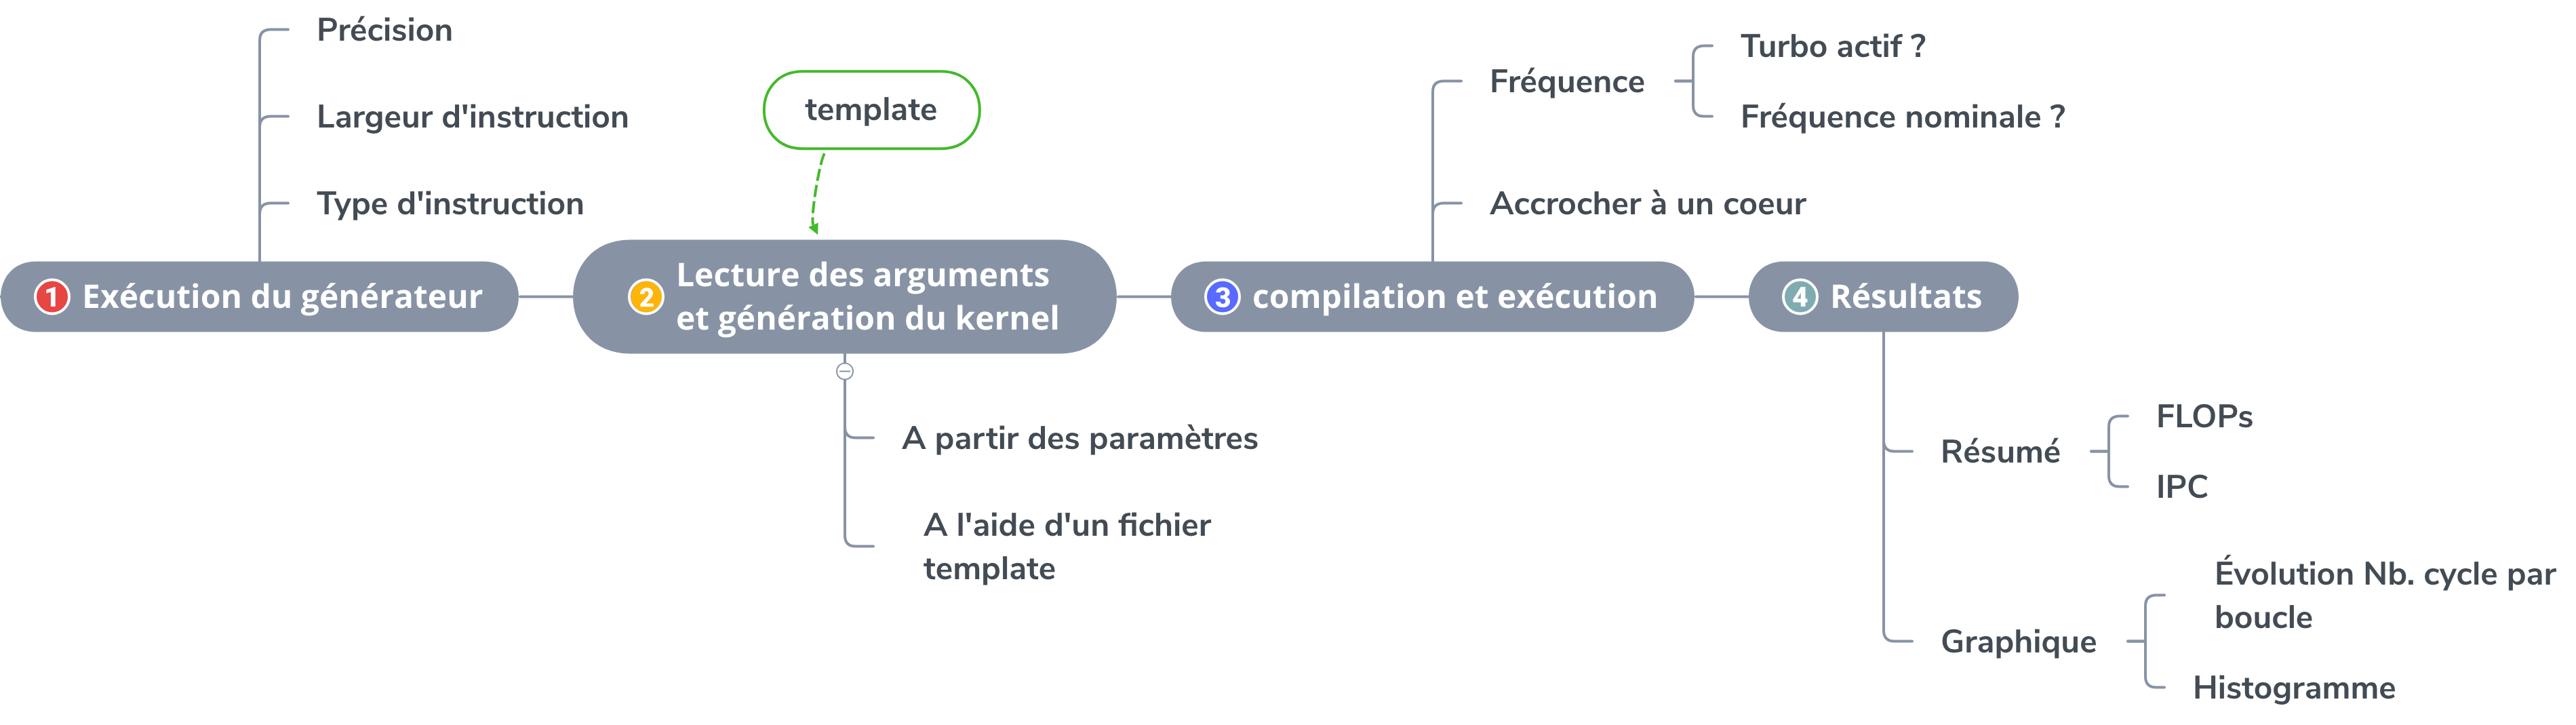
\includegraphics[width=16cm]{images/kg_workflow.png}
            \caption{\label{pic_kg_workflow} Déroulement de l'exécution du générateur de kernels.}
            \end{figure}
    
            Le générateur de kernels accepte plusieurs options lui permettant de produire différents benchmarks. La commande suivante montre un exemple d'utilisation du générateur: \verb|./kg   -P double -W 128  -O aamm|. Cette commande permet de générer un kernel de calculs utilisant quatre instructions vectorielles de 128 bits sur des nombres flottant en double précision. Le kernel est composé de quatre instructions (deux additions et deux multiplications):
        \begin{verbatim}
"vaddpd %%xmm0, %%xmm1, %%xmm2;"
"vaddpd %%xmm0, %%xmm1, %%xmm3;"
"vmulpd %%xmm0, %%xmm1, %%xmm4;"
"vmulpd %%xmm0, %%xmm1, %%xmm5;"
        \end{verbatim}
        
      
        
    
    \subsubsection{Génération du benchmark}
    %%%%%%%%%%%%%%%%%%%%%%
        
        Une fois les différentes options analysées, le générateur va écrire un programme C++ contenant le benchmark à exécuter. Tous les benchmarks ont une partie commune de code qui est stockée dans un fichier \textit{template}. Le générateur s'occupe seulement d'écrire la partie en assembleur dans ce fichier et d'initialiser quelques variables (nombre de mesures, coeur sur lequel s'exécuter). Le \textit{template} contient le code permettant de mesurer les résultats, de calculer la fréquence et d'afficher le résultat  dans le terminal. Un exemple d'exécution du générateur est résumé sur la \autoref{pic_kg_generation}. Le code généré par l'outil reste simple pour faciliter les conclusions que pourra tirer son utilisateur. En effet, produire un code trop complexe rendrait l'analyse des résultats trop difficile sur des  architectures aussi complexes que celles étudiées. 

        \begin{figure}[h!]
            \center
            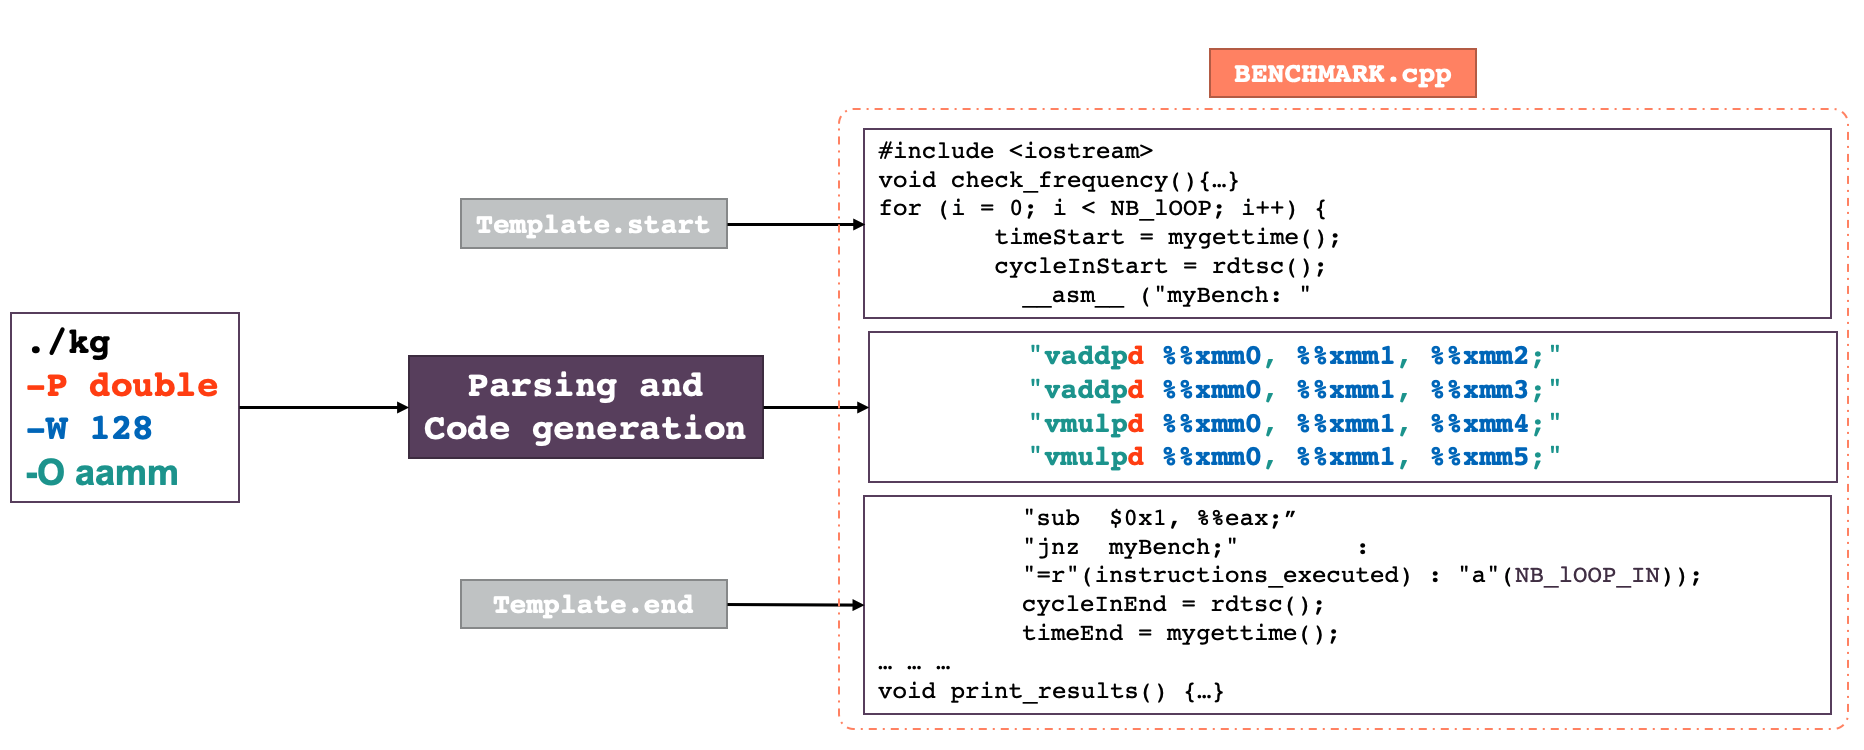
\includegraphics[width=16cm]{images/kg_generation.png}
            \caption{\label{pic_kg_generation}Génération du benchmark à partir de la ligne de commande entrée par l'utilisateur. La partie commune du code est stockée dans un fichier de \textit{template}.}
        \end{figure}
        

    \subsubsection{Exécution du benchmark}
    %%%%%%%%%%%%%%%%%%%%%%

        Une fois le code du benchmark généré (voir \autoref{pic_kg_generation}), celui-ci est compilé automatiquement par le générateur (le compilateur peut être modifié facilement). Le code et le benchmark peuvent ensuite être utilisés  sans passer de nouveau par le générateur. Ces deux fichiers sont créés dans le dossier courant de l'utilisateur. Un exemple de résultat de l'exécution du benchmark est présenté ci-dessous:
    
    
 \begin{lstlisting}[label=output:basic_gflops ,language=, caption=Exemple d'exécution d'un benchmark de quatre instruction AVX-512.]
./kg -W 512 -O aamm -P double -U 4 -S 30000 -L 500000

--------------------  CHECK FREQUENCY  ------------------------
+ Base      frequency is 2.69GHz
+ Current   frequency is 2.68GHz
+ OK: the core is running at his frequency based value

------------------  INSTRUCTIONS SUMMARY -----------------------
_label_|   NB INSTRUCTIONS      Time    FREQUENCY       Giga_inst/sec       IPC
_value_|      240000000000      44.7         2.69                5.37      1.99

----------------------  FLOP SUMMARY  --------------------------
 PRECISION     FLOP/cycle         FLOP/second
    Single              0                   0
    Double             16             4.3e+10
----------------------------------------------------------------


\end{lstlisting}   
    
        Le benchmark généré comporte quatre instructions vectorielles AVX-512: deux additions et deux multiplications. Le processeur utilisé est un  Intel Xeon 6150 cadencé à 2.70GHz. Pour cette expérimentation le turbo a été désactivé. Pour améliorer la précision des résultats, la boucle générée est déroulée 4 fois. La boucle réalise 500000 itérations et sa performance est mesurée 30000 fois. Le CPU est capable d'exécuter deux opérations flottantes vectorielles par cycle d'horloge. Pour des données en doubles précisions, cela correspond à réaliser 16 opérations flottantes par cycle. La puissance de calcul atteinte par le benchmark généré est de 43 GFLOPs. Pour chaque mesure le nombre de cycles et le temps nécessaire à l'exécution de la boucle sont sauvés dans un fichier. Ce fichier peut ensuite être affichée avec un script python (voir \autoref{fig:kg_graph}). La \autoref{pic_kg_plot} permet de voir comment la performance du benchmark évolue au fil des exécutions. On peut détecter des problèmes de détériorèrent des performances pouvant être dus à un mauvais refroidissement du processeur par exemple.  La \autoref{pic_kg_hist} affiche l'histogramme permettant de voir deux familles de performances.
        
        \begin{figure}
            \centering
            \begin{subfigure}[b]{0.45\linewidth}
                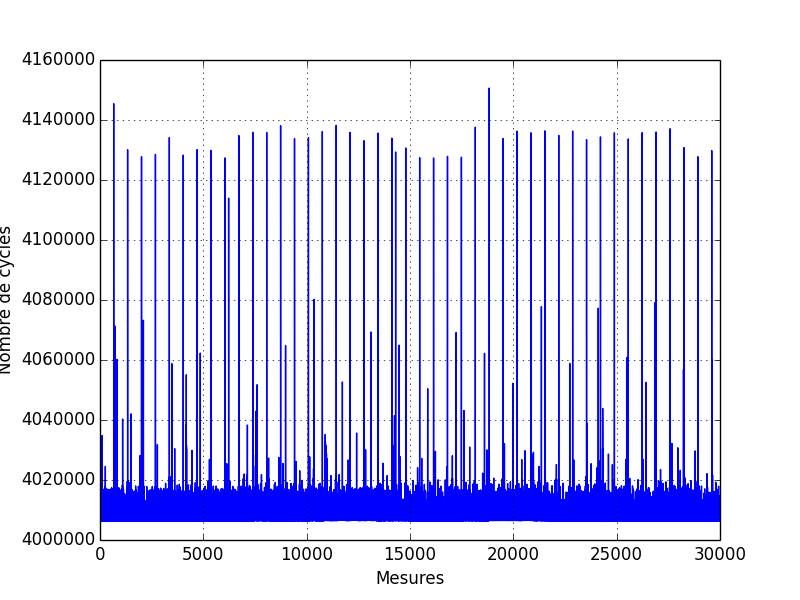
\includegraphics[width=\linewidth]{images/kg_plot.png}
                \caption{Évolution du nombre de cycles nécessaire pour l'exécution de la boucle de benchmark}
                \label{pic_kg_plot}
            \end{subfigure}
            ~ %add desired spacing between images, e. g. ~, \quad, \qquad, \hfill etc. 
              %(or a blank line to force the subfigure onto a new line)
            \begin{subfigure}[b]{0.45\linewidth}
                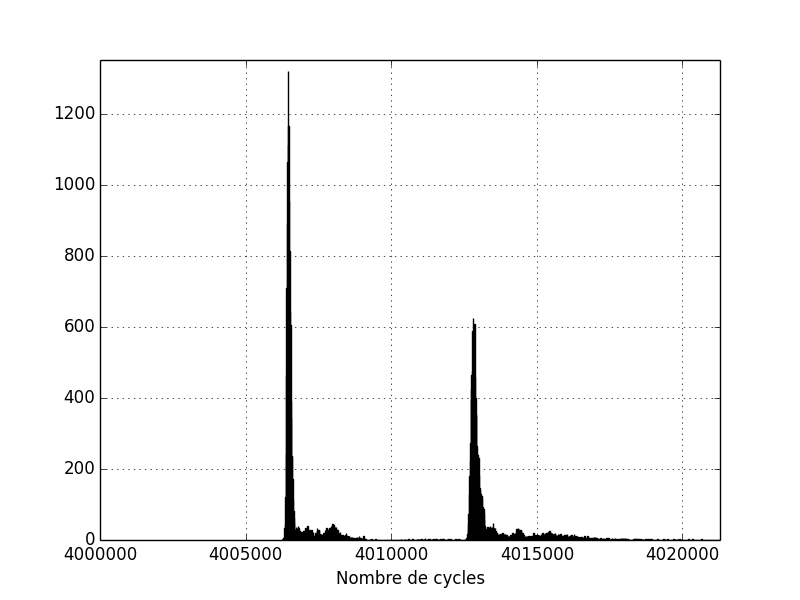
\includegraphics[width=\linewidth]{images/kg_hist.png}
                \caption{Histogramme du nombre de cycles nécessaire}
                \label{pic_kg_hist}
            \end{subfigure}
            \caption{Grâce à un script python, le fichier de résultat peut être affiché sous forme de graphique. }\label{fig:kg_graph}
        \end{figure}
    
  
        %%%% OPTION %%%    
        \subsubsection{Les options.} 
        
            Une des forces du générateur vient de sa faculté à générer un grand nombre de benchmarks différents. Ceci est possible grâce à l'utilisation des différentes options dont les principales sont expliquées dans cette sous-section.
        
            Grâce à l'option \verb|--operation {a,m,f}| l'utilisateur donne une chaîne de caractères pour choisir  les opérations à réaliser (addition (a), multiplication (m) ou FMA (f)). Différentes opérations peuvent être mixées et sont ensuite exécutées dans le même ordre. Dans cet exemple, les quatre instructions sont composées de deux additions et de deux multiplications. Cette option associée à un second script permet de générer des kernels testant différentes combinaisons d'opérations en changeant la chaîne de caractère, composée de \textit{a, m} ou \textit{f}. En faisant varier à la fois les opérations et la taille des instructions, l'outil permet de découvrir des comportements cachés des architectures.
    
            Le benchmark peut être exécuté pour réaliser des calculs en simple ou double précision grâce à l'option \verb|--precision {single, double}|. 
            La largeur des instructions vectorielle est choisie grâce à l'option \verb|--width {64, 128, 256, 512}|. Elles peuvent utiliser différentes ISA: MMX (64), SSE (128), AVX (256) ou AVX-512 (512). 
            
            L'option \verb|--dependency {N}| permet de générer une instruction  dont un opérande est le résultat produit par l'instruction précédente. Un nombre $N$ peut être donné pour générer plusieurs chaînes de dépendances non dépendantes entre elles. Cette option est particulièrement utile pour mesurer la latence des instructions et la performance du tampon d'exécution dans le désordre.
            
            L'option \verb|--binding N| est utilisée pour accrocher le benchmark généré à un coeur spécifique. Le benchmark n'étant pas parallélisé il est nécessaire d'en exécuter plusieurs versions en parallèle pour tester la performance d'un processeur lorsque plusieurs coeurs sont utilisés.
            
            L'option \verb|--unroll N| permet d'appliquer l'optimisation du déroulement de boucle N fois. Cette optimisation permet de dérouler plusieurs fois le corps de la boucle à l'intérieur de celle-ci pour réduire l'impact du traitement des instructions de contrôle de la boucle (incrémentation et comparaison) sur les performances du benchmark. 
            
            L'option \verb|--frequency| permet de générer et d'exécuter une fonction en début de benchmark qui mesure la fréquence du processeur. Les calculs des résultats sont impactés par l'utilisation du mode turbo. En connaissant la valeur de la fréquence turbo, ces résultats peuvent être ajustés. En effet, la mesure de la performance du benchmark est réalisée en utilisant la valeur de la fréquence de base du processeur. 
            
            Pour améliorer la précision des résultats et éliminer les potentiels bruits de mesure, l'utilisateur peut indiquer le nombre $N$ de mesures à réaliser grâce à l'option \verb|--loopsize N|.    
    
    
    \subsubsection{Validation des résultats}
    
        Lors du développement du générateur, il a été nécessaire d'utiliser des outils nous permettant de valider les performances rapportées par le benchmark. Pour s'assurer du bon fonctionnement du benchmark sur de nouvelles architectures, certaines de ces méthodes de vérification ont été implémentées dans l'outil directement. 
        
        
        %#TODO enelver le compteur je pense qu'il est NDA pour HPE
        \paragraph{Validation du nombre d'instructions.} La première valeur à valider est de s'assurer que le bon nombre d'instructions a été exécuté par le benchmark. Le benchmark affiche le nombre d'instructions qui devrait être exécuté. Un moyen de le vérifier est d'utiliser les compteurs matériels. L'outil \textit{perf} permet de mesurer le nombre d'évènements d'un compteur en utilisant son adresse (une instruction FMA compte pour deux). La ligne de commande suivante permet de compter les opérations flottantes réalisées par le benchmark: \verb|perf stat -e /rffc7 ./benchmark|. Le résultat du benchmark ci-dessus prévoyait l'exécution de 240,000,000,000 opérations. La commande \verb|perf stat| retourne une valeur de 240,000,210,024 opérations. Pour comprendre d'où proviennent les instructions supplémentaires, nous avons mesuré différentes versions du benchmark avec différentes longueurs de boucle (5000, 10000 et 20000). Le \autoref{tab:kg_vs_perf} donne les résultats affichés par le benchmark et par la commande précédente utilisant l'outil \textit{perf}. Les résultats de \textit{perf} mesure le bon nombre d'instructions avec 2124 opérations supplémentaires à chaque fois. Ces instructions supplémentaires correspondent en fait au traitement des résultats..
    
        \begin{table}[h!]
        \centering
        \resizebox{\textwidth}{!}{%
        \begin{tabular}{@{}lcc@{}}
        \toprule
         & Nombre d'instructions & Résultat perf \\ \midrule
        ./kg -W 512 -O aamm -P double -S 300 -L 5000 & 6000000 & 6002124 \\
        ./kg -W 512 -O aamm -P double -S 300 -L 10000 & 12000000 & 12002124 \\
        ./kg -W 512 -O aamm -P double -S 300 -L 20000 & 24000000 & 24002124 \\ \bottomrule
        \end{tabular}%
        }
        \caption{Vérification du nombre d'instructions exécutées avec l'outil perf.}
        \label{tab:kg_vs_perf}
        \end{table}
        
        
        
        \paragraph{Validation de l'IPC.} La validation de l'IPC peut elle aussi être réalisé grâce à perf et la commande \verb|perf stat ./benchmark|. Pour générer le benchmark la commande suivante a été utilisée: \verb|./kg -W 512 -O aamm -P double -S 1000 -L 90000000|. Pour que les instructions vectorielles prennent la plus grande partie du temps de l'exécution, la taille de la boucle a été allongée. Le benchmark donne alors un IPC de 2 alors que la commande \textit{perf} donne un résultat de 3. Cette différence peut être expliqué en regardant le code assembleur généré (voir \autoref{lst:kg:ipc}). 
        
        \begin{lstlisting}[label=lst:kg:ipc ,language=C, caption=Code généré par la commande ./kg -W 512 -O aamm -P double]
cycleInStart = rdtsc();
__asm__ ("" 
    "myBench: " 
		"vaddpd %%zmm0, %%zmm1, %%zmm2; "
		"vaddpd %%zmm0, %%zmm1, %%zmm3; "
		"vmulpd %%zmm0, %%zmm1, %%zmm4; "
		"vmulpd %%zmm0, %%zmm1, %%zmm5; "
    "sub  $0x1, %%eax;"
    "jnz  myBench;"		: "=r" (instructions_executed) : "a" (NB_lOOP_IN));
cycleInEnd = rdtsc();
\end{lstlisting}
        
        Notre calcul d'IPC ne prend en considération que les instructions de calculs alors que \textit{perf} compte la totalité des instructions exécutées. Notre calcul prend pour postulat que les deux instructions de gestion de boucle (la décrémentation \verb|sub|, et le saut conditionnel \verb|jnz|) ne rentre pas dans le profil de l'exécution. Grâce au prédicateur de branchement, l'instruction de saut peut effectivement être enlevée de nos calculs. Concernant la soustraction, nous avons réalisé un test pour vérifier l'impact de soustraction de nombre entier lors de l'exécution d'un code ne réalisant que des opérations sur des nombres flottants (voir \autoref{code:sub}). 
        
        \begin{lstlisting}[label=code:sub ,language=C, caption=Mesure de l'impact de la soustraction]
"myBench: " 
 "vfmadd231pd %%zmm0, %%zmm1, %%zmm2; "
 "vfmadd231pd %%zmm0, %%zmm1, %%zmm3; "
 "vfmadd231pd %%zmm0, %%zmm1, %%zmm4; "
 "vfmadd231pd %%zmm0, %%zmm1, %%zmm5; "
 "sub  $0x1, %%ebx;" //fake substraction
 "sub  $0x1, %%ebx;" //fake substraction
 "sub  $0x1, %%ebx;" //fake substraction
 "sub  $0x1, %%eax;" 
"jnz  myBench;"	  
        \end{lstlisting}
        
        
        En mesurant la performance de ce code, nous avons mesuré que 4 soustractions sur des nombres entiers n'impactent pas la performance de la boucle. Au-delà de 4, le processeur a besoin de cycles supplémentaires pour les exécuter. Ainsi les deux instructions de gestion de boucles peuvent être ignorées de notre calcul. Pour réduire l'impacte de ces deux instructions sur le résultat donnée par \textit{perf}, nous avons implémenté une option de déroulement de boucle (\textit{unrolling}). La commande suivante déroule le code 10 fois permettant de valider le calcul d'IPC du benchmark avec la valeur donnée par \textit{perf}: \verb|kg -W 512 -O aamm -P double -S 10 -L 900000000 -U 10 |.
        
        
        
        
        \paragraph{Validation des FLOPS.} La première méthode a été d'utiliser un outil développé en interne appelé \textit{mygflops}. Cet outil affiche le nombre d'opérations exécutées en consultant les compteurs matériels de chaque coeur. Le résultat sépare les différentes tailles d'instructions vectorielles utilisées. La commande, le résultat du benchmark et celui de \textit{mygflops} sont présentés dans l'\autoref{lst:basic_gflops}. 
        
\begin{lstlisting}[label=lst:basic_gflops ,language=C, caption=Validation des résultats donnés par le benchmark grâce à l'outil \textit{mygflops}.]
./kg -W 128 -O aamm -P double -U 10 -S 10 -L 90000000
...
----------------------  FLOP SUMMARY  --------------------------
 PRECISION     FLOP/cycle         FLOP/second
    Single              0                   0
    Double           4.00            1.06e+10
----------------------------------------------------------------
...

********************** MYGFLOPS ***********************
     
Single-precision SSE/AVX :            0.000000 GFlop/s --  0.0% of Flops

       0.0%  32-bit SSE/AVX instructions (0.0%)
       0.0% 128-bit SSE/AVX instructions (0.0%)
       0.0% 256-bit AVX instructions     (0.0%)
       0.0% 512-bit AVX instructions     (0.0%)
     
Double-precision SSE/AVX :            10.572521 GFlop/s -- 100.0% of Flops

       0.0%  64-bit SSE/AVX instructions (  0.0%)
     100.0% 128-bit SSE/AVX instructions (100.0%)
       0.0% 256-bit AVX instructions     (  0.0%)
       0.0% 512-bit AVX instructions     (  0.0%)

\end{lstlisting}
        
        Cependant, cet outil n'est pas disponible en accès libre pour le reste de la communauté. Nous avons ainsi développé une méthode de validation des résultats internes au benchmark. En fonction des opérations utilisées, les registres sont initialisés avec différentes valeurs significatives. Par exemple, pour vérifier que le bon nombre d'additions a été exécuté, les registres sont initialisés à la valeur 1. À la fin du benchmark, les registres ayant participé au benchmark sont sommés pour vérifier que le bon nombre d'additions a été exécuté. Grâce à cette méthode, nous avons la certitude que les opérations sont réellement exécutées par le processeur et qu'aucune optimisation lui permettant d'en éviter n'est possible. 
        

    
    \subsubsection{Mesure de la fréquence}
    %%%%%%%%%%%%%%%%%%%%%%
        Plus un processeur utilise une fréquence élevée, plus sa consommation électrique est élevée. Pour cette raison, Intel a adopté différents niveaux de fréquence pour ses processeurs. Cela permet d'augmenter les performances en cas de besoin et de limiter la consommation d'énergie si le processeur n'a pas besoin d'être pleinement utilisé. L'instruction \verb|rdtsc| est utilisée pour lire le compteur matériel correspondant au nombre de \textit{tics} depuis la dernière réinitialisation du processeur \cite{code:rdtsc}. La fréquence correspond à la fréquence de base nominale du processeur et est indépendante de la fréquence d'horloge réelle pouvant varier. Si les fréquences des processeurs devaient varier, les mesures effectuées avec \verb|rdtsc| seraient erronées. C'est pourquoi la fréquence du processeur doit être choisie avant l'exécution du micro-benchmark. Dans le cas d'une fréquence fixe différente de la fréquence de base nominale, nous avons mis en place une vérification qui calculera ensuite cette fréquence, et ajustera les résultats mesurés par \verb|rdtsc| comme le calcul de l'IPC. Cette fonctionnalité de vérification de la fréquence et de la correction de résultat est utilisable avec l'option \verb|-F true|. 
        
        \paragraph{Mesurer la fréquence de base.} Nous avons développé un code pour mesurer la fréquence de base. Il utilise la fonction \textit{sleep} qui attend un certain nombre de microsecondes ainsi que l'instruction \verb|rdtsc|. Ainsi nous pouvons calculer la fréquence avec le rapport $cycleSpent / timeSpent$ comme indiqué sur \autoref{code:base_freq}. 
        

\begin{lstlisting}[label=code:base_freq ,language=C, caption=Code used to measure the base frequency of the processor]
timeStart = mygettime();
cycleInStart = rdtsc();
    usleep(10000);
cycleInEnd = rdtsc();
timeEnd = mygettime();
cycleSpent = (cycleInEnd - cycleInStart);
freq_Base = cycleSpent / (1000000000 * (timeEnd - timeStart));
\end{lstlisting}        

        \paragraph{Mesurer la fréquence réelle.} Pour pouvoir ajuster les résultats affichés par le benchmark, il est nécessaire de connaître la fréquence à laquelle le processeur est capable d'aller. Cette fréquence peut varier en fonction de l'utilisation du mode \textit{turbo} ou si la fréquence a été limitée de façon logicielle. Pour réaliser cette mesure, nous sommes partis du constat que tous les processeurs modernes sont capables d'exécuter une soustraction sur un registre par cycle d'horloge. Dans l'\autoref{code:cur_freq}, le registre \verb|%eax| est initialisé à \verb|80000000|. Grâce à notre hypothèse, il est possible de prévoir que le processeur réalisera ces \verb|80000000| soustractions en autant de cycles. Nous mesurons le nombre de cycles à \textit{fréquence nominale} passé dans l'exécution de cette boucle. En faisant le rapport entre le nombre de cycles mesurés et celui attendu grâce à notre hypothèse, il est possible de déterminer si le processeur utilise une fréquence plus ou moins rapide que sa fréquence nominale. Nous calculons ainsi l'IPC de cette boucle en faisant le rapport $\frac{80000000}{cycleSpent}$.
        \begin{itemize}
            \item \verb|IPC == 1|: Le processeur utilise sa fréquence de base
            \item \verb|IPC < 1|: Le processeur utilise une fréquence inférieur à sa fréquence de base.
            \item \verb|IPC > 1|: Le processeur est capable d'exécuter des instructions à une fréquence plus élevée que sa fréquence de base (turbo).
        \end{itemize}
    
\begin{lstlisting}[label=code:cur_freq ,language=C, caption=Mesure de la fréquence de base du processeur]
cycleInStart = rdtsc();
__asm__ ("aloop: "
    "sub $0x1,%%eax;"
    "sub $0x1,%%eax;"
    "sub $0x1,%%eax;"
    "sub $0x1,%%eax;"
    "jnz aloop" : : "a" (80000000UL)
);
cycleInEnd = rdtsc();
cycleSpent = (cycleInEnd - cycleInStart);
\end{lstlisting}   
    
    
        \paragraph{Ajuster les résultats.} En connaissant la fréquence de base et la fréquence accessible par le processeur les résultats donnés par le benchmark peuvent être ajustés. Nous avons utilisé un script externe pour verrouiller la fréquence du processeur Intel Xeon 6150 à 2.00 GHz. Ce processeur a une fréquence de base de 2.70GHz. Notre code présenté dans la section précédente mesure un IPC pour le code du \autoref{code:cur_freq} de 0.742. Cela signifie qu'il fonctionne actuellement à 74,2\% de sa fréquence de base, soit 2,00 GHz. Ce premier test permet de valider la méthodologie basée sur \verb|rdtsc|, mais aussi pour valider avant toute expérimentation que la fréquence est correctement réglée. Grâce à l'option \verb|--frequency true| le générateur fera cette vérification pour ajuster les résultats donnés par \verb|rdtsc|. 
        
    
    
    
    
    
    
\subsection{Résultats}
%%%%%%%%%%%%%%%%%%%%%%%%%%%%%%%%%%%%%%%%%%%%%%%%%%%%%
    Nous présentons dans cette section comment le générateur peut être utilisé pour caractériser une plate-forme ainsi que les résultats obtenus pendant les travaux de thèse.
   
   
   

    \subsubsection{Vérifier les performances théoriques}
    %%%%%%%%%%%%%%%%%%%%%%%%%%%%%%%%%%%%%%%%%%%%%%%%%%%%%
    Le générateur de kernel peut être utilisé pour vérifier ou mesurer les performances maximales atteignables par un processeur. Pour illustrer cette utilisation, nous avons étudié les performances du processeur Intel Xeon 6150 cadencé à 2.7 GHz, possédant 18 coeurs et disposant d'un mode Turbo. Les résultats de cette expérimentation sont donnés dans le \autoref{tab:kg_vs_intel}. Pour chaque configuration (nombre de coeurs, type d'instruction, turbo activé) Intel donne dans sa documentation les différentes fréquences supportées par le processeur\footnote{\url{https://www.intel.com/content/dam/www/public/us/en/documents/specification-updates/xeon-scalable-spec-update.pdf}}. Lorsque le turbo est désactivé, la fréquence du processeur pour exécuter un type d'instruction ne varie pas en fonction du nombre de coeurs utilisés. Cette fréquence est appelée \textit{Base Core Frequency} (BCF). Cette fréquence est également la fréquence minimale qui peut être atteinte par un processeur doté d'un système de refroidissement correctement configuré. Cette fréquence peut donc être utilisée pour calculer une limite inférieure de la performance du processeur. Cependant la fréquence BCF donnée par Intel est une fréquence garantie. Si la température et la conception du processeur le permettent, le processeur peut utiliser des fréquences plus élevées. Le but de cette expérimentation est d'utiliser le générateur de kernel pour mesurer cette fréquence et ainsi déterminer la performance maximale théorique lorsque le turbo est désactivé. 
    Pour connaître la borne supérieure de la performance maximale du processeur, il faut lire attentivement la documentation pour en relever les valeurs présentées sur la quatrième ligne du \autoref{tab:kg_vs_intel} (colonne \textit{Turbo ON}). Cette fréquence est appelée \textit{Maximum Core Frequency} (MCF). Cette fréquence n'est pas garantie, et est seulement atteignable si la température du processeur le permet. En fonction de sa qualité de fabrication (fuite de courant) et de l'efficacité de son système de refroidissement, la fréquence MCF peut varier de 20\%.  

    
    La performance maximale atteignable (en GFLOPs) pour chaque type d'instruction (Non-AVX, AVX 2.0 et AVX-512) peut être mesurée en exécutant des instructions FMA. Nous avons utilisé le générateur de kernel pour créer des benchmarks utilisant trois tailles d'instructions (scalaire, 256 et 512 bits) avec la commande suivante:
\begin{lstlisting}
./kg -W {64,256, 512} -O ffffffffffffff -P double -U 80 -S 1 -L 90000000
\end{lstlisting}


    \begin{table}[h!]
    \centering
    \resizebox{\textwidth}{!}{%
    \begin{tabular}{|l|cc|cc|cc|cc|cc|cc|}
    \hline
    Jeu d'instruction & \multicolumn{4}{c|}{\cellcolor[HTML]{67FD9A}Non-AVX} & \multicolumn{4}{c|}{\cellcolor[HTML]{34FF34}AVX 2.0} & \multicolumn{4}{c|}{\cellcolor[HTML]{009901}AVX 512} \\ \hline
    Turbo & \multicolumn{2}{c|}{\cellcolor[HTML]{FFFFC7}OFF} & \multicolumn{2}{c|}{\cellcolor[HTML]{FCFF2F}ON} & \multicolumn{2}{c|}{\cellcolor[HTML]{FFFFC7}OFF} & \multicolumn{2}{c|}{\cellcolor[HTML]{FCFF2F}ON} & \multicolumn{2}{c|}{\cellcolor[HTML]{FFFFC7}OFF} & \multicolumn{2}{c|}{\cellcolor[HTML]{FCFF2F}ON} \\ \hline
    Nombre de coeurs & \multicolumn{1}{c|}{\cellcolor[HTML]{ECF4FF}1} & \cellcolor[HTML]{CBCEFB}18 & \multicolumn{1}{c|}{\cellcolor[HTML]{ECF4FF}1} & \cellcolor[HTML]{CBCEFB}18 & \multicolumn{1}{c|}{\cellcolor[HTML]{ECF4FF}1} & \cellcolor[HTML]{CBCEFB}18 & \multicolumn{1}{c|}{\cellcolor[HTML]{ECF4FF}1} & \cellcolor[HTML]{CBCEFB}18 & \multicolumn{1}{c|}{\cellcolor[HTML]{ECF4FF}1} & \cellcolor[HTML]{CBCEFB}18 & \multicolumn{1}{c|}{\cellcolor[HTML]{ECF4FF}1} & \cellcolor[HTML]{CBCEFB}18 \\ \hline
    \rowcolor[HTML]{EFEFEF} 
    Fréquence (GHz) (source Intel) & 2.7 & 2.7 & 3.7 & 3.4 & 2.3 & 2.3 & 3.6 & 3.0 & 1.9 & 1.9 & 3.5 & 2.5 \\ \cline{1-1}
    \rowcolor[HTML]{EFEFEF} 
    Performance théorique (GFLOPs) & 10.8 & 194.4 & 14.8 & 244.8 & 36.8 & 662.4 & 57.6 & 864 & 60.8 & 1094 & 112 & 1440 \\ \hline
    \rowcolor[HTML]{FFE4E2} 
    Performance KG (GFLOPs) & 10.8 & 192.6 & 14.8 & 244.2 & 43 & 772.2 & 57.3 & 858.8 & 86 & 1430 & 112 & 1430 \\ \cline{1-1} 
    \rowcolor[HTML]{FFE4E2} 
    Fréquence calculée (GHz) & 2.7 & 2.7 & 3.7 & 3.4 & {\color[HTML]{00009B} \textbf{2.68}} & {\color[HTML]{00009B} \textbf{2.68}} & 3.58 & {\color[HTML]{000000} 2.97} & {\color[HTML]{00009B} \textbf{2.68}} & {\color[HTML]{00009B} \textbf{2.48}} & 3.5 & 2.48 \\ \hline
    \end{tabular}%
    }
            \caption{
            Mesure de la performance du processeur Intel 6150 utilisant trois jeux d'instructions, avec et sans Turbo et en utilisant un seul ou tous les coeurs. Les données mesurées (en rouge) sont à comparer avec les spécifications techniques données par le constructeur (en gris). Intel communique les fréquences minimales garanties pour chaque cas. Cependant, les performances réelles peuvent être supérieures (en bleu) lorsque le processeur est capable de soutenir une fréquence plus élevée (consommation électrique, chaleur).}
            \label{tab:kg_vs_intel}
    \end{table}
    
    
    Quelle que soit la taille de l'instruction, le processeur Skylake étudié est capable d'exécuter deux instructions par cycles. Ces instructions nécessitant plus ou moins de transistors pour être exécutées (taille, nombre de coeur) le processeur doit adapter sa fréquence pour ne pas surchauffer.  Le Kernel Generator mesure le nombre d'instructions par cycle, ce qui nous permet de vérifier que deux instructions FMA sont bien exécuter chaque cycle. Le benchmark calcule aussi la performance en GFLOPs du code. Grâce à ces deux informations, il est possible de calculer la fréquence réelle qu'utilise le processeur (dernière ligne du  \autoref{tab:kg_vs_intel}). Nous remarquons en bleu, quatre fréquences supérieures à celle annoncée par la documentation. En effet, Intel communique la fréquence minimale garantie pour chaque configuration (turbo, nombre de coeurs, type d'instructions). Cette fréquence minimale est garantie pour tous les processeurs d'un même modèle (même SKU). La qualité de fabrication du processeur peut lui permettre d'atteindre des fréquences plus élevées que celle-ci, comme indiqué en bleu dans le \autoref{tab:kg_vs_intel}. Pour étudier l'évolution de la fréquence et de la température du processeur, nous utilisons un outil développé en interne par HPE. La \autoref{pic_kg_freq_vs_temp} montre que le processeur est capable d'utiliser une fréquence de 2.7 GHz, alors que la fréquence minimale garantie est de 2.3 GHz. Le benchmark a été exécuté pendant trente minutes. Le bon système de refroidissement utilisé empêche le processeur de dépasser sa puissance TDP (Thermal Design Ppower) et de conserver cette fréquence durant toute l'exécution. La puissance TDP est mesurée en watt et exprime la quantité de chaleur dégagée par le processeur lorsqu'il est en charge. Le TDP permet au constructeur de système de refroidissement de calibrer le matériel nécessaire pour refroidir un processeur.  
    
           
    \begin{figure}[!h]
        \centering
        \begin{subfigure}[t]{0.45\linewidth}
            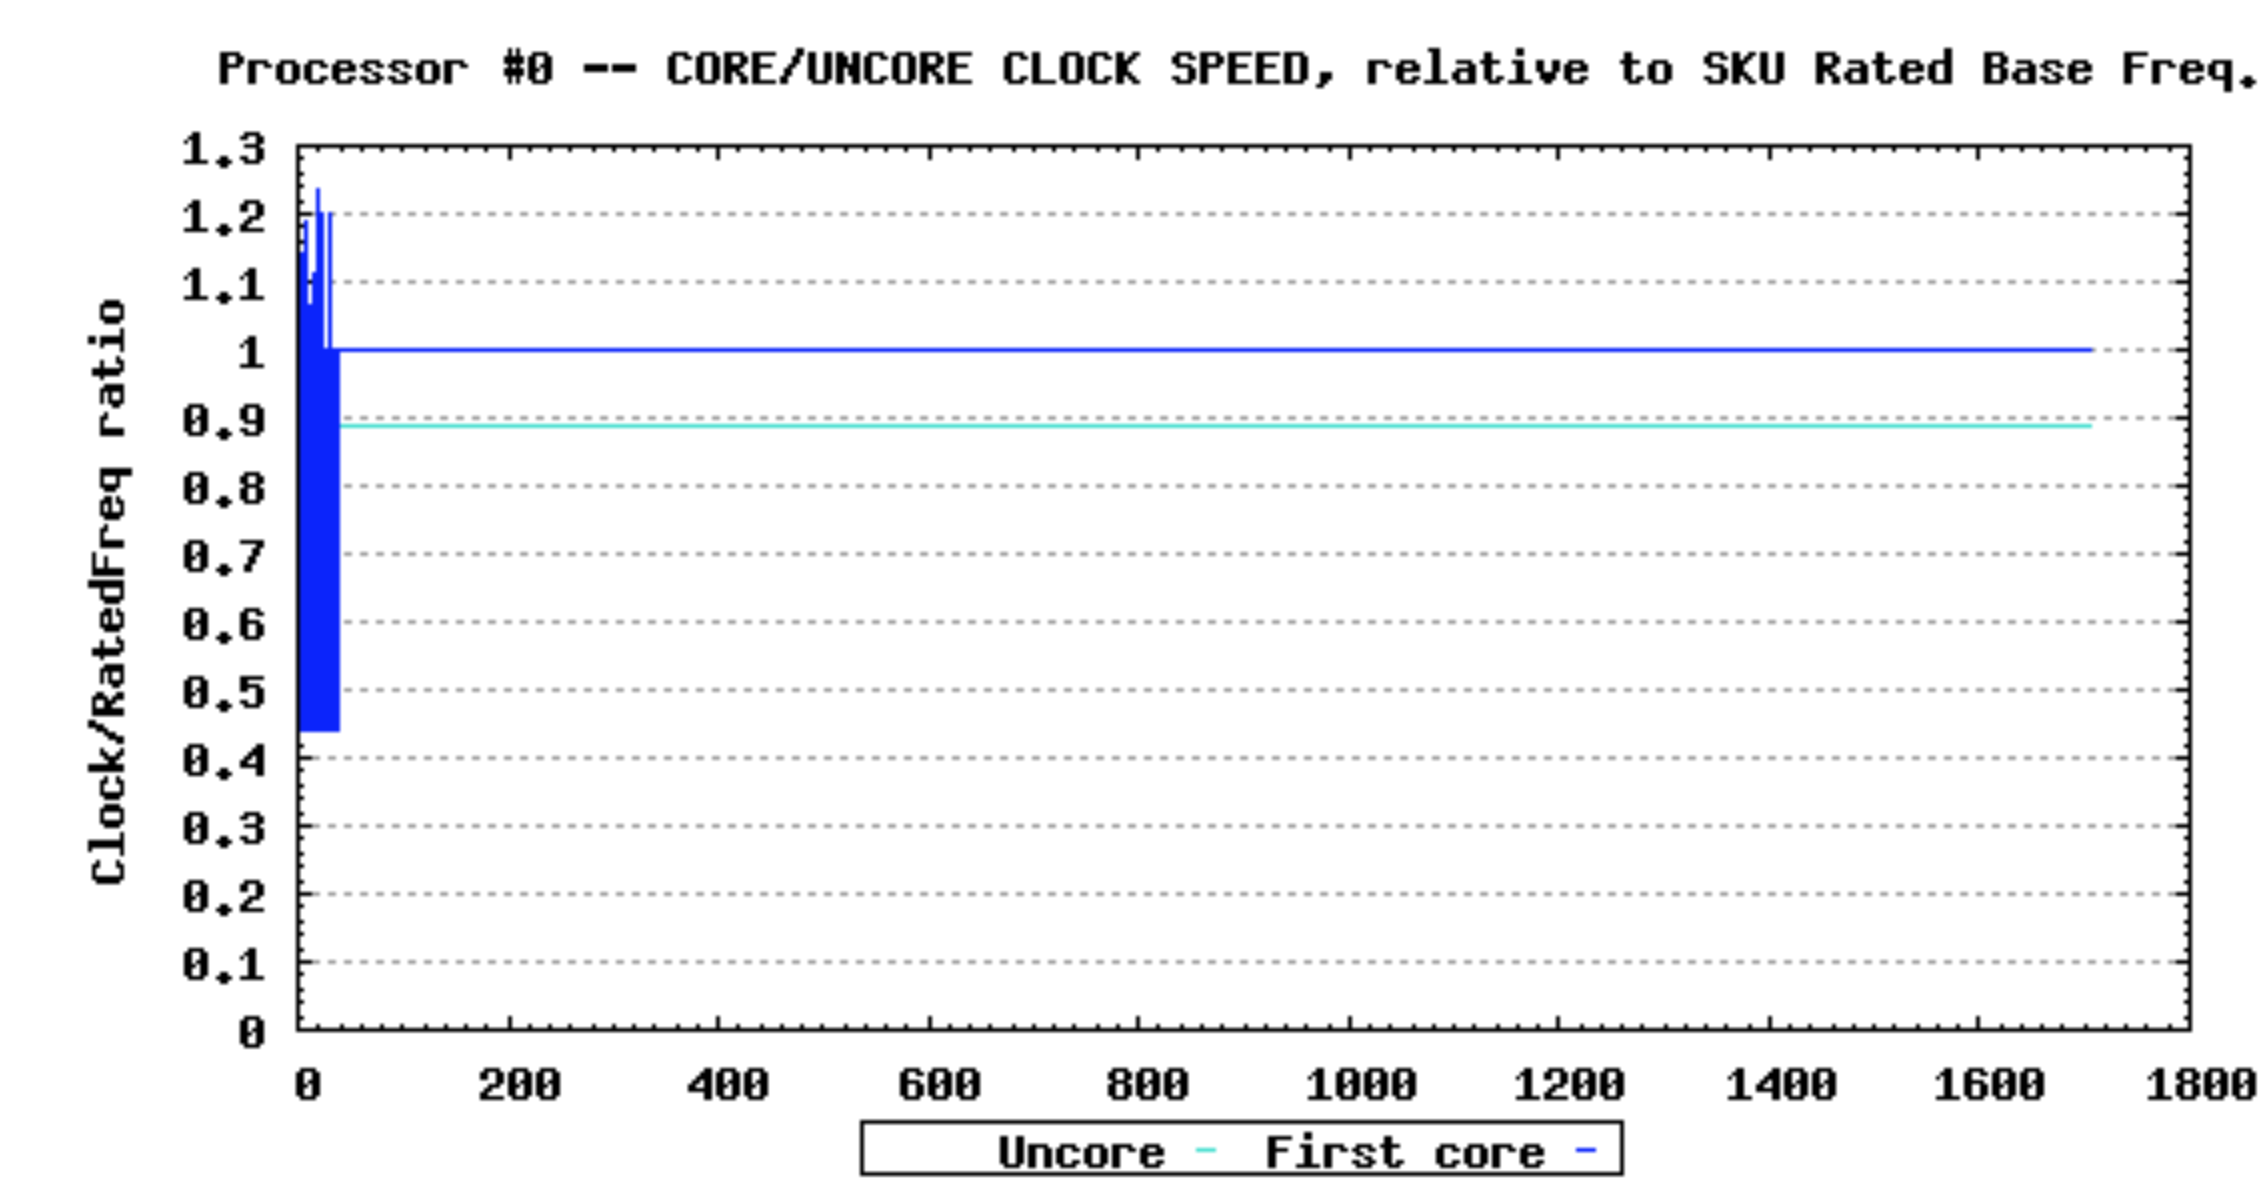
\includegraphics[width=\linewidth]{images/kg_freq.png}
            \caption{Évolution de la fréquence. Un ratio de 1 correspond à la fréquence de base de processeur (2.7 GHz).}
            \label{pic_kg_freq}
        \end{subfigure}
        ~ %add desired spacing between images, e. g. ~, \quad, \qquad, \hfill etc. 
          %(or a blank line to force the subfigure onto a new line)
        \begin{subfigure}[t]{0.45\linewidth}
            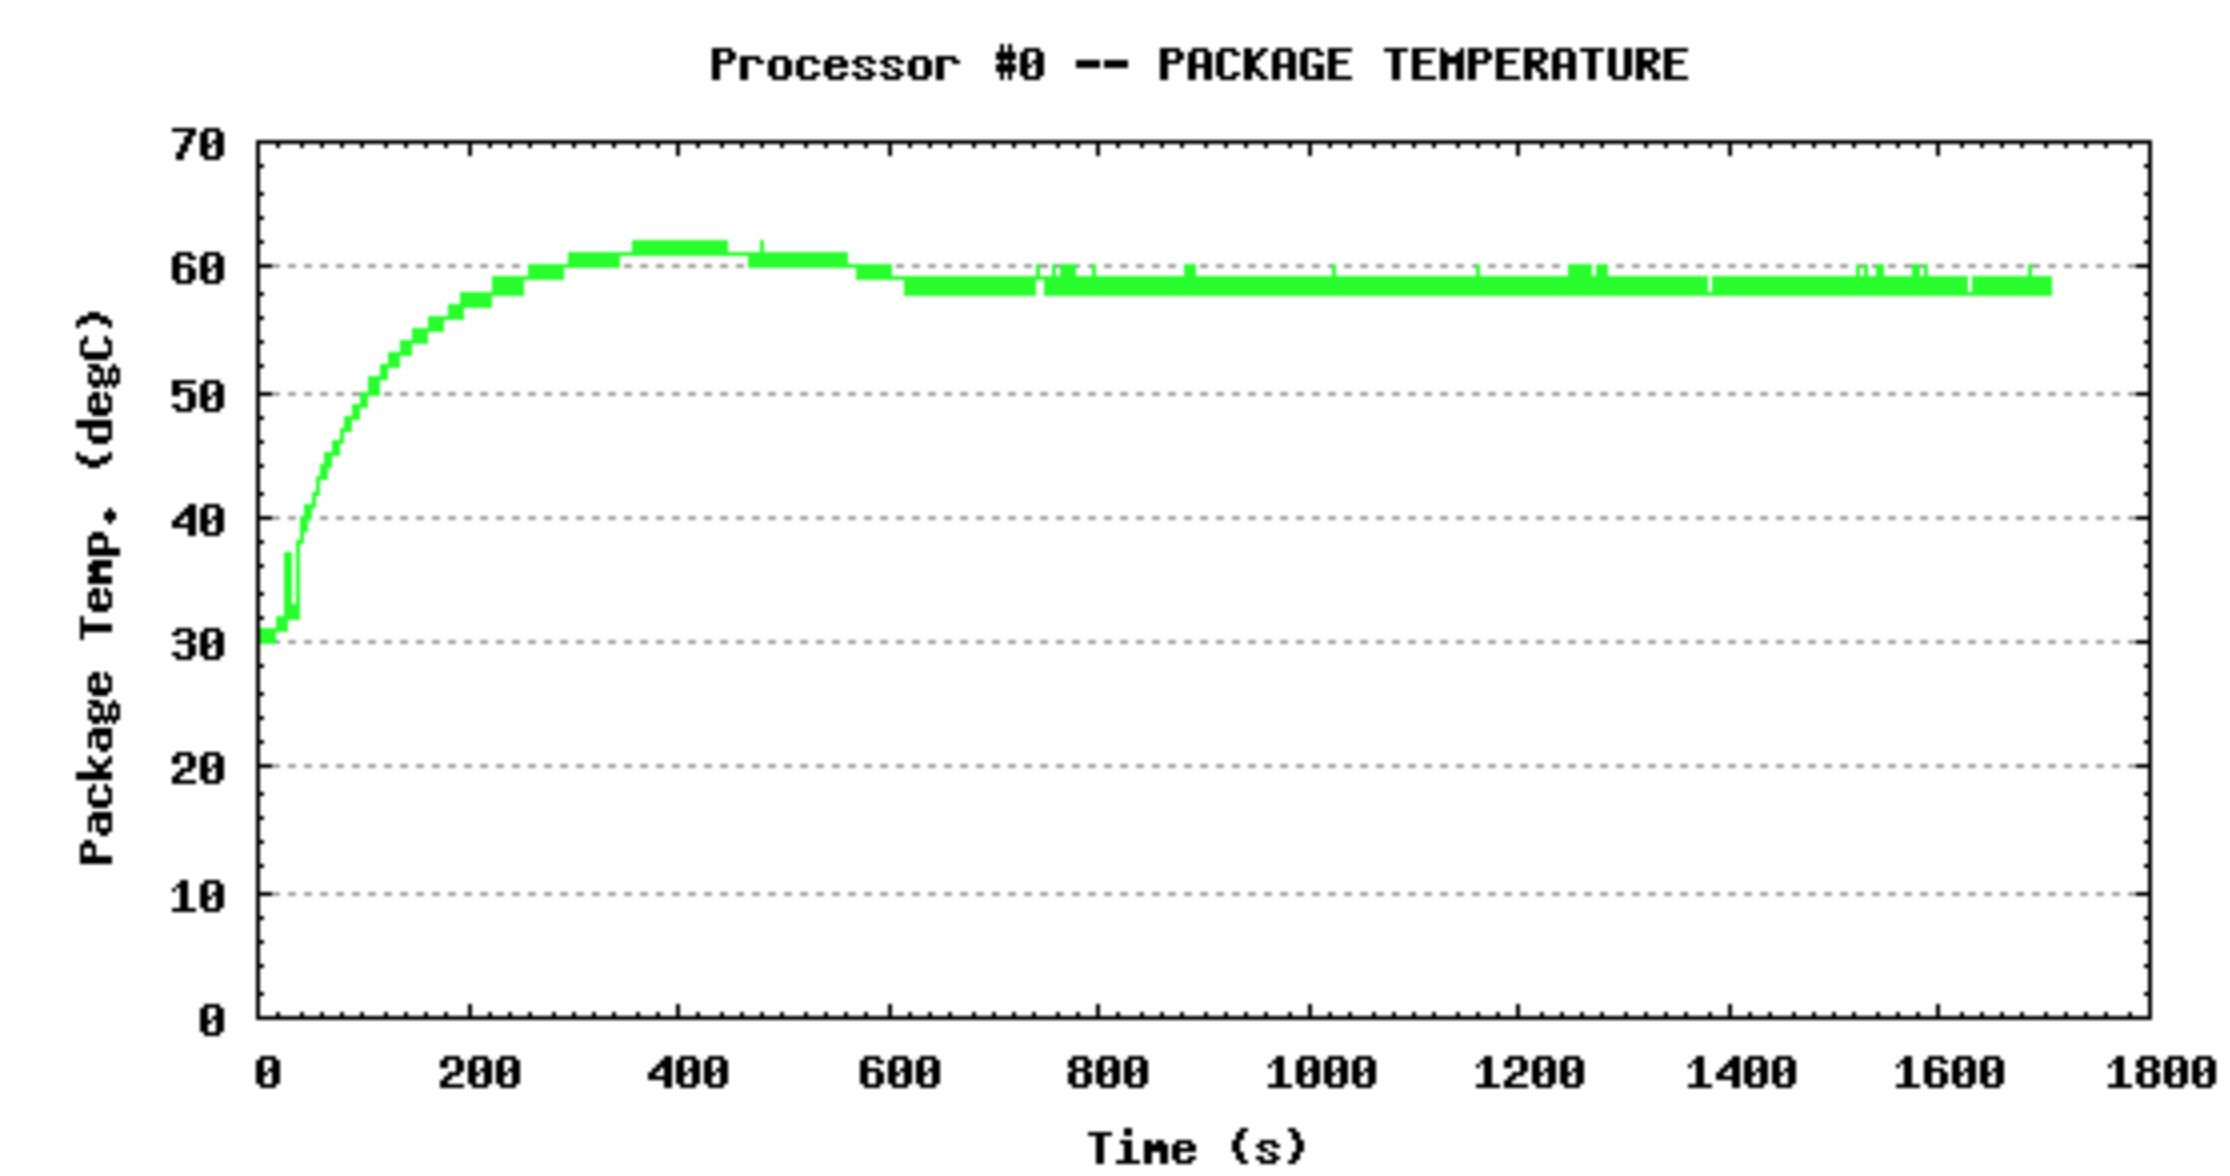
\includegraphics[width=\linewidth]{images/kg_temp.png}
            \caption{Évolution de la température du processeur}
            \label{pic_kg_temp}
        \end{subfigure}
        \caption{Évolution de la fréquence et de la température du processeur pour un benchmark AVX 2.0 exécuté sur 18 coeurs avec le turbo désactivé}\label{pic_kg_freq_vs_temp}
    \end{figure}

        




    
    \subsubsection{Caractérisation de la micro-architecture Haswell}
    %%%%%%%%%%%%%%%%%%%%%%%%%%%%%%%%%%%%%%%%%%%%%%%%%%%%%
    Lors de l'utilisation d'une nouvelle plate-forme, l'utilisateur peut utiliser le générateur de benchmark pour caractériser la microarchitecture et trouver ses points forts ou points faibles. Lors de l'arrivée des processeurs Intel de génération Haswell en 2013, certains codes ont connu des baisses de performances malgré l'utilisation d'une architecture plus récente. Nous avons utilisé le générateur de kernels pour caractériser les performances d'exécution des additions et des multiplications avec la commande suivante : \verb|./kg  -P double -W 64 -O mmmmm| permettant de générer le benchmark suivant:
    
    \begin{lstlisting}[label=lst:kg_mul ,language=C]
for (i = 0; i < NB_lOOP; i++) {
timeStart = mygettime();
cycleInStart = rdtsc();
__asm__ ("" 
     "myBench:"  
   		"vmulsd %%xmm0, %%xmm1, %%xmm2; "
   		"vmulsd %%xmm0, %%xmm1, %%xmm3; "
   		"vmulsd %%xmm0, %%xmm1, %%xmm4; "
   		"vmulsd %%xmm0, %%xmm1, %%xmm5; "
   		"vmulsd %%xmm0, %%xmm1, %%xmm6; "
     "sub  $0x1, %%eax;"
     "jnz  myBench;"		:: "a" (NB_lOOP_IN));
cycleInEnd = rdtsc();
timeEnd = mygettime();
cycle_total += (cycleInEnd - cycleInStart);
time_total += timeEnd - timeStart;
}
\end{lstlisting}
    
     La microarchitecture Haswell est capable d'exécuter deux multiplication par cycle. Cependant, l'utilisation du générateur de kernel nous a montré que le processeur n'était pas capable d'exécuter des additions au même rythme que les multiplications. Les résultats présentés dans le \autoref{tab:mul_vs_add} montrent que la microarchitecture Haswell est capable d'exécuter deux multiplications contre une seule addition par cycle.

    \begin{table}[h!]
    \centering
    \begin{tabular}{|l|c|c|c|c|}
        \hline
        Opération & Nombre d'instructions & Frequence & Temps & IPC \\ \hline
        Multiplication & 40000000000 & 2.1 & 7.71 & \textbf{2} \\ \hline
        Addition & 40000000000 & 2.1 & 14.43 & {\color[HTML]{963400} \textbf{1}} \\ \hline
        \end{tabular}%
        
        \caption{Différence de performance lors de l'exécution d'addition et de multiplication sur une architecture Haswell.}
        \label{tab:mul_vs_add}
    \end{table}
    
    Bien sûr, cette caractéristique est documentée et en comptant le nombre de ports destiné aux additions, l'utilisateur du processeur aurait pu en trouver la raison. Cependant la lecture de la documentation de la microarchitecture dépasse le millier de pages et en comprendre les moindres détails est plus difficile que d'utiliser les bons outils. Nous pensons que le générateur de benchmark peut permettre à n'importe quel utilisateur de rapidement trouver ce genre de caractéristiques. Avant même d'avoir exécuté son application sur une nouvelle plate-forme, il peut rapidement se faire une idée de ses performances et trouver ce genre de défauts.




    \subsubsection{Caractérisation de l'exécution dans le désordre}
    %%%%%%%%%%%%%%%%%%%%%%%%%%%%%%%%%%%%%%%%%%%%%%%%%%%%%

    La puissance d'un supercalculateur vient de sa capacité à réaliser des calculs en parallèle. Pour satisfaire la loi d'Amdahl (voir \autoref{sec:amdhal}), les développeurs essaient de maximiser les zones de codes pouvant profiter des ressources parallèles des architectures. Le principal frein à l'utilisation du parallélisme vient de zones de code dit séquentiel. Ces lignes de codes doivent être exécutées à la suite les unes des autres, car par exemple, une de ces instructions nécessite d'avoir le résultat de la précédente. Les performances d'un tel code peuvent être très mauvaises, mais la nature des algorithmes peut assez fréquemment laisser place à certaines optimisations. Dans le domaine des finances, les algorithmes de Monte-Carlo sont très utilisés. Ces codes ont la particularité d'exposer de longues chaînes de dépendance. En restructurant le code, le programmeur peut espérer profiter de l'exécution dans le désordre (voir \autoref{sec:out_of_order}). Cela nécessite cependant d'apporter suffisamment d'instructions indépendantes au processeur pour qu'il puisse les exécuter. Le processeur est capable d'exécuter plusieurs chaînes indépendantes les unes des autres. La performance d'une telle plate-forme dépend alors de sa capacité à en suivre plus ou moins en parallèle. Grâce à l'option \verb|--dependency N| du générateur de kernels, le benchmark peut être utilisé pour caractériser cette fonctionnalité matérielle. Cette option permet de générer plusieurs chaînes indépendantes. En utilisant une dépendance de 1, chaque instruction a besoin du résultat de l'instruction précédente (voir \autoref{lst_dep1}). Dans ce cas-là, aucune parallélisation n'est possible pour le processeur.
    
    
\begin{lstlisting}[label=lst_dep1,language=C, caption=Code généré par la commande /kg -W 512 -P double -O mmmmm -D 1]
"myBench: " 
	"vmulpd %%zmm0, %%zmm6, %%zmm2; "
	"vmulpd %%zmm0, %%zmm2, %%zmm3; "
	"vmulpd %%zmm0, %%zmm3, %%zmm4; "
	"vmulpd %%zmm0, %%zmm4, %%zmm5; "
	"vmulpd %%zmm0, %%zmm5, %%zmm6; "
"sub  $0x1, %%eax;"
"jnz  myBench;"
\end{lstlisting}

    La performance atteinte par ce code est de 0.25 instruction par cycle d'horloge. Le processeur a besoin de 4 cycles d'horloge pour exécuter une instruction. Cette latence vient de la nécessité d'attendre que le résultat de l'opération précédente soit disponible pour pouvoir commencer à être exécuté. 
    
    En ajoutant des chaînes de dépendances grâce à l'option \verb|--dependecy N|, nous avons pu valider que le processeur est capable d'exécuter au moins 8 chaînes d'instructions indépendantes. Le code généré pour 4 chaînes est présenté sur la \autoref{pic_kg_dep_4}. En faisant varier le nombre de chaînes indépendantes, les résultats présentés dans le \autoref{tab_kg_depth} ont été obtenus. Grâce au tampon d'instructions de système d'exécution dans le désordre, le processeur est capable de commencer l'exécution de plusieurs chaînes indépendantes simultanément. Le processeur peut exécuter une multiplication par cycle par pipeline (2 au total). La latence d'une multiplication AVX-512 étant de 4 cycles, le processeur a besoin de 8 chaînes indépendantes pour utiliser la totalité de la puissance du processeur. Cette caractéristique du processeur doit être connue par le programmeur pour transformer son code et obtenir le maximum de performance du processeur. Grâce au générateur de kernels, les nouvelles architectures peuvent être testées pour caractériser ces performances et prévoir leur performance pour des codes pouvant utiliser des chaînes de calculs indépendantes comme la résolution de polynômes par exemple. 
    
         \begin{figure}
            \center
            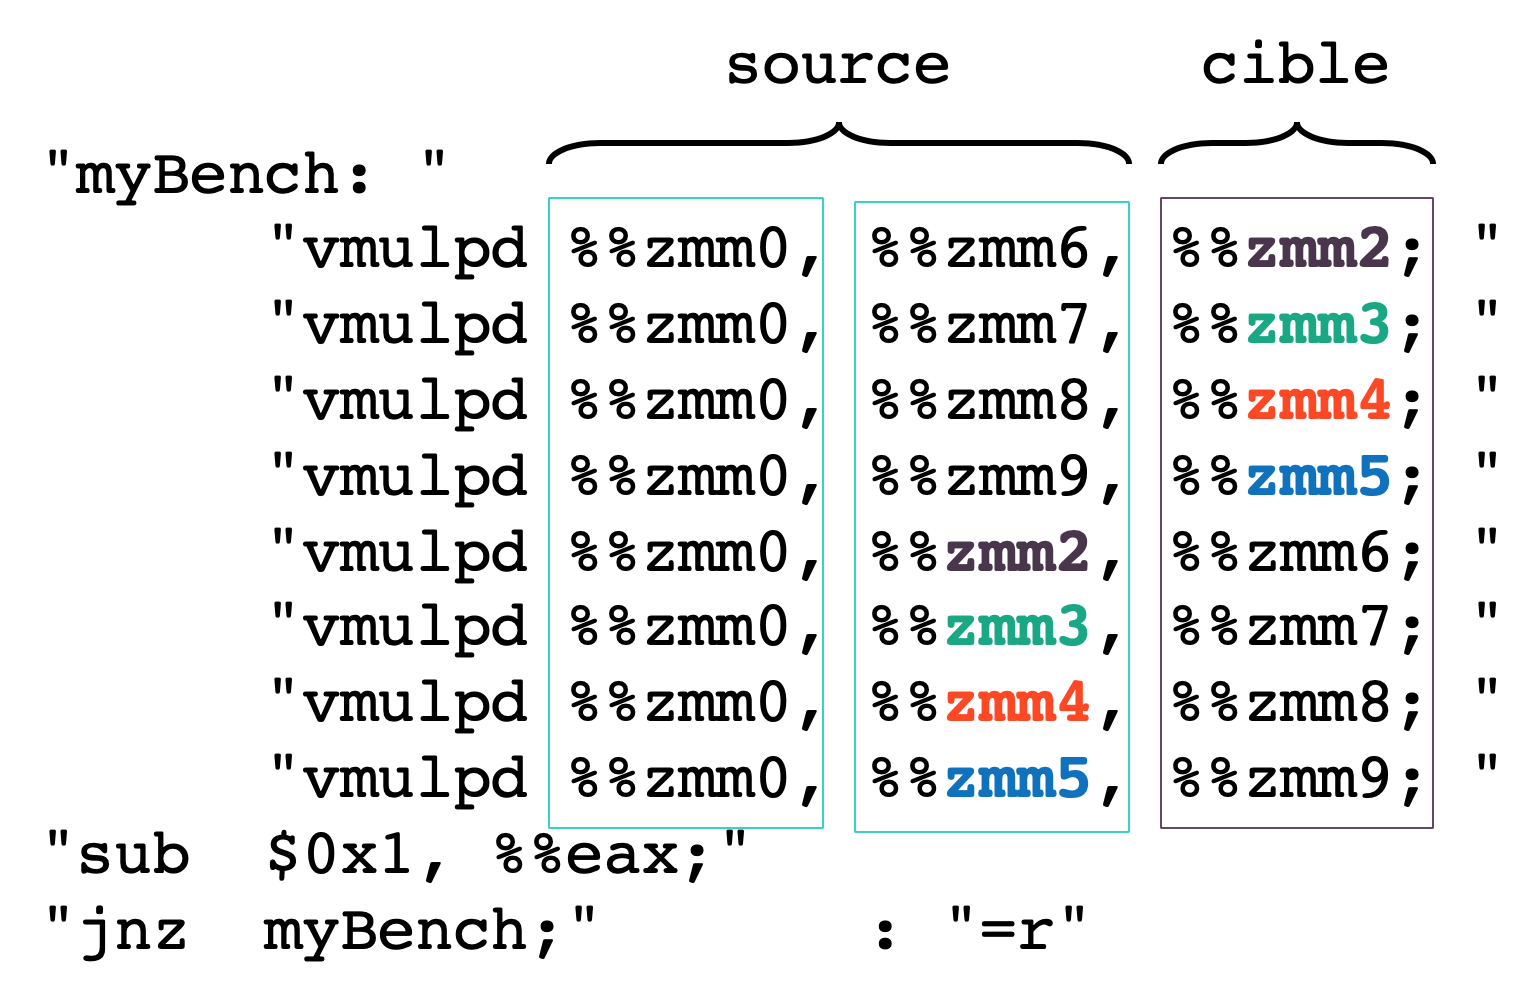
\includegraphics[width=8cm]{images/kg_dep_4.png}
            \caption{\label{pic_kg_dep_4} Code généré par la commande /kg -W 512 -P double -O mmmmmmmm -D 4}
        \end{figure}

    \begin{table}[h!]
    \centering
    \normalsize
    \begin{tabular}{|l|c|c|c|c|c|c|c|c|c|c|}
    \hline
    Nombre de chaînes & 1 & 2 & 3 & 4 & 5 & 6 & 7 & 8 & 9 & 10 \\ \hline
    IPC & 0.25 & 0.50 & 0.75 & 1 & 1.25 & 1.50 & 1.75 & 2 & 2 & 2 \\ \hline
    \end{tabular}%
    \caption{Impact du nombre de chaînes pouvant être exécutées indépendamment sur la performance du code (mesurée en Instruction Par Cycle).}
    \label{tab_kg_depth}
    \end{table}





    \subsubsection{Caractérisation de la FPU de deux processeurs Skylake}

        Pour caractériser la performance crêtes des processeurs, notre équipe de benchmark utilise des codes tels que HPL. Pour obtenir la meilleure performance atteignable, le benchmark est compilé pour utiliser les instructions vectorielles les plus grandes (AVX-512) (voir \autoref{table:skl_bench}). La dernière génération de processeur Intel Skylake est répartie en quatre gammes (bronze, silver, gold et platinium). Les fonctionnalités et les performances des processeurs des différentes gammes étant différentes (voir \autoref{table:skl}), il est important pour notre équipe avant-vente d'en connaître les caractéristiques et les performances pour adapter les configurations des serveurs aux demandes clients. Les processeurs des gammes bronze ou silver sont rarement choisis pour répondre à un appel d'offres compte tenu de leurs caractéristiques plus faibles (une FPU au lieu de deux, nombre plus faible de coeurs).
        
        
        \begin{table}[h!]
        \centering
        \caption{Skylake portfolio: différences principales des SKUs}
        \label{table:skl}
        \resizebox{\textwidth}{!}{%
        \begin{tabular}{|l|l|l|l|l|l|}
        \hline
        \rowcolor[HTML]{EFEFEF}
                                        &   Bronze: 31XX                    & Silver: 41XX              & Gold: 5100            & Gold: 6100            & Platinium: 8100           \\ \hline
        Memory channel and speed    & 6-ch@2133 Ghz                         & 6-ch\textbf{@2400}      & 6-ch@2400           & 6-ch\textbf{@2666}   & 6-ch@2666                \\ \hline
        UPI links (Scalability)         &     2   (2S-2UPI)       & 2  (2S-2UPI)    & 2 (4S-2UPI)  & 3  (2S-3UPI) & 3    (8S-3UPI)    \\ \hline
        UPI bandwidth                   & 9.6 GT/s                          & 9.6 GT/s                  & 10.4 GT/s              & 10.4 GT/s             & 10.4 GT/s                 \\ \hline
        HyperThreading  \cite{Marr2002}                &   NO                              & \textbf{YES}              & YES                   & YES                   & YES                       \\ \hline
        FMA-512 FPU                     &     1                             & 1                         & 1                     & \textbf{2 }           & 2                         \\ \hline
        
        \end{tabular}
        }
        
        \end{table}
        
        
      Les résultats du benchmark Linpack donnés dans le \autoref{table:skl_bench}, montrent que les processeurs les plus performants sont ceux appartenant aux gammes Gold et Platinium. Ces processeurs possèdent généralement plus de coeurs, et sont capables d'utiliser des fréquences plus élevées que les processeurs d'entrée de gamme. Bien sûr, comme ces processeurs coûtent plus cher à l'achat, un client choisira un processeur en fonction de son budget, de sa consommation électrique ou du profile de son application. Cette différence de performance peut être expliquée par la présence de deux FPU sur les processeurs haut de gamme. Ces deux FPU sont capables d'exécuter chacune une instruction FMA en AVX-512 par cycle. Grâce au générateur de kernel, cette caractéristique a pu être vérifiée (voir \autoref{table:skl_bench}).

        \begin{table}[h!]
        \centering
        \caption{Skylake performance the HPL Benchmark in GFLOP/s: 8 process per core, HyperThreading off, frequency capped at 1.5 Ghz) \textbf{todo: refaire full core no capping}}
        \label{table:skl_bench}
        \resizebox{\textwidth}{!}{%
        \begin{tabular}{|l|l|l|l|l|}
        \hline
        \rowcolor[HTML]{EFEFEF}
        Processeur (Nb. FPU)    & Silver: 4110 (1)  & Gold: 5117 (1)   & Gold: 6130 (2)    & Platinium: 8160 (2)        \\ \hline
        HPL (512)            & 297           & 372          & 714           & 716                  \\ \hline
        AVX-512 FMA par cycle   & 1             & 1            & 2             & 2                    \\ \hline
        \end{tabular}
        }
        \end{table}
        
        
        Afin d'estimer l'impact d'une FPU manquante sur la performance, nous avons utilisé une application de CFD typique. L'application utilisée n'exécute que des instructions vectorielles de 256 bits. Nous nous attendons alors à obtenir des performances différentes entre un processeur Silver et Gold pour une application qui n'est pas limitée par la bande passante mémoire. Étonnamment, les résultats obtenus sur ces deux plates-formes sont très proches. Pourtant, nous avons bien montré que les processeurs de gamme supérieure possèdent une FPU de plus et sont donc deux fois plus performants. 

        Pour comprendre ce phénomène, nous avons utilisé le générateur de benchmark pour générer un kernel de calculs utilisant des instructions AVX de 256 bits.    


        \begin{verbatim}
./kg  -P double -W 256 -O ffffffff -F true
        \end{verbatim}
        
        \begin{table}[h!]
        \centering
        % increase table row spacing, adjust to taste
        %\renewcommand{\arraystretch}{1.1}
        % COMMENTS if using array.sty, it might be a good idea to tweak the value of
        %\extrarowheight{1} as needed to properly center the text within the cells
        \caption{Xeon Gold and Silver results for AVX2 instructions}
        \label{table:skl_bench2}
        \resizebox{0.4\textwidth}{!}{%
        \begin{tabular}{|l|l|l|l|l|}
        \hline
        \rowcolor[HTML]{EFEFEF}
                                & Silver: 4110       & Gold: 6130      \\ \hline
        IPC                     & 2                  & 2           \\ \hline
        GFLOP/s                 & 2.38e+10           & 2.37e+10           \\ \hline
        \end{tabular}
        }
        \end{table}
        
        La performance mesurée pour le kernel AVX-2 sont reportés dans le \autoref{table:skl_bench2}.  Bien que le processeur Intel Xeon Silver 4110 ne possède qu'une seule FPU, il est capable d'exécuter deux instructions AVX-2 par cycle. Cette caractéristique peut être retrouvée dans la documentation du processeur \footnote{source: \url{https://en.wikichip.org/wiki/intel/microarchitectures/skylake\#Execution_engine_2}}. Les FPU des processeurs Skylake d'entrée de gamme fusionnent deux ports de 256 bits pour former la FPU 512-bits. Cependant, lorsque des instructions de 256 bits sont exécutées, le processeur peut utiliser les deux ports indépendamment pour exécuter deux instructions. La FPU supplémentaire sur les processeurs haut de gamme est une FPU 512 bits qui ne permet pas d'utiliser cette caractéristique et d'exécuter (en théorie) quatre instructions par cycle. 

        Nous avons ensuite poussé la caractérisation des FPU des processeur Silver plus loin pour vérifier comment la fusion de la FPU fonctionnait. Pour cela, le générateur de benchmark a de nouveau été utilisé grâce à l'option permettant de mixer différentes tailles d'instructions vectorielles. Les résultats reportés dans le \autoref{res:skl} ont pu être trouvés. La FPU est capable chaque cycle d'exécuter: 


        \begin{itemize}
            \item Une instruction AVX 512 bits.
            \item Deux instruction AVX 256 bits.
            \item Deux instructions AVX 128 bits.
            \item Deux instructions scalaire.
            \item Toutes combinaisons de deux instructions dont la taille agrégée ne dépasse pas 512 bits.
        \end{itemize}
        
        
        \begin{table}[h!]
        \normalsize
        % increase table row spacing, adjust to taste
        %\renewcommand{\arraystretch}{1.1}
        % COMMENTS if using array.sty, it might be a good idea to tweak the value of
        %\extrarowheight{1} as needed to properly center the text within the cells
        \caption{Nombre d'instruction exécuté chaque cycle pour différentes gamme de processeurs en mixant différentes tailles d'instructions.}
        \label{res:skl}
        \centering
        %\resizebox{\textwidth}{!}{%
        \begin{tabular}{|l|c|c|c|c|}
            \hline
            \rowcolor[HTML]{EFEFEF} 
            Gamme & Silver & Gold & Gold & Platinium \\ \hline
            \rowcolor[HTML]{EFEFEF} 
            Ref. processeur Intel Skylake & 4110 & 5117 & 6130 & 8160 \\ \hline
            \rowcolor[HTML]{EFEFEF} 
            Nombre de FPU & 1 & 1 & 2 & 2 \\ \hline
            128 + scalaire & \textbf{2} & \textbf{2} & 2 & 2 \\ \hline
            256 + scalaire & \textbf{2} & \textbf{2} & 2 & 2 \\ \hline
            256 + 128 & \textbf{2} & \textbf{2} & 2 & 2 \\ \hline
            256 & \textbf{2} & \textbf{2} & 2 & 2 \\ \hline
            512 + scalaire & 1 & 1 & 2 & 2 \\ \hline
            512 + 128 & 1 & 1 & 2 & 2 \\ \hline
            512 + 256 & 1 & 1 & 2 & 2 \\ \hline
        
        \end{tabular}
        %}
        \end{table}
        
        
        
       Ainsi, le processeur haut de gamme bénéficie des deux FPU lorsque le code est capable d'utiliser des instructions vectorielles de 512 bits. Il est fréquent que les applications n'y parviennent pas (mauvaise vectorisation du code, problème du compilateur, dépendances) et utilisent des instructions vectorielles plus petites, les processeurs d'entrée de gamme obtiennent des performances rigoureusement égales. Évidement, la FPU n'est pas la seule responsable de la performance d'une application, le \autoref{table:skl} montrent bien que d'autres caractéristiques diffèrent telles que le nombre de liens UPI ou la possibilité d'utiliser l'Hyperthrading . Le but du générateur de kernel est de caractériser une architecture pour le besoin d'une application. Plusieurs réponses à des offres d'appels ont été réalisées avec des processeurs d'entrée de gamme. Grâce à cette caractéristique, les applications utilisant des instructions AVX-2 peuvent obtenir des performances assez proches sur des processeurs coûtant beaucoup moins cher.


        
        




%    \subsubsection{Expliquer les performances d'un code}
    %%%%%%%%%%%%%%%%%%%%%%%%%%%%%%%%%%%%%%%%%%%%%%%%%%%%%
 %   Une autre utilisation du générateur de kernel peut permettre d'expliquer les performances d'une autre application. 
    
    
  %   What we have seen in the past months with the releases of the new Skylake processors is that entry level processors like Intel 4110 can perform as good as a top bin processor like the Intel 6148 for real applications thus increasing the $\frac{performance}{price}$ of a large scale cluster. 



    
    %%%%%%%%%%%%%%%%%%%%%%%%%%%%%%%%%%%%%%%%%%%%%%%%%%%%%



\subsection{Conclusion}
%%%%%%%%%%%%%%%%%%%%%%%%%%%%%%%%%%%%%%%%%%%%%%%%%%%%%
    
    Le générateur de kernel assembleur est un outil très précis pour la caractérisation des FPUs. Le principal avantage de l'utilisation de l'assembleur est d'éviter au maximum les optimisations du compilateur. Le benchmark doit assurer à l'utilisateur qu'il mesure bien la performance du code qu'il a choisi de générer et qu'il n'a pas été modifié durant la compilation. Il nous a permis d'atteindre des performances souvent égales aux performances théoriques. 
    
    Pour le moment, seul l'ISA x86 est supporté, mais l'outil a été codé de façon à faciliter l'ajout d'une nouvelle ISA. Nous avons choisi de commencer à le développer pour des processeurs dont nous connaissons bien le comportement pour valider son bon fonctionnement. L'exemple de la FPU du processeur Intel Xeon 4110, nous a permis de montrer que même sur des architectures que nous connaissons bien, certaines spécificités nous échappent encore. L'utilisation du générateur permet d'en comprendre toutes les particularités.
    
    Il est connu que la performance des applications actuelles est principalement limitée par le système mémoire. Ainsi, nous avons constaté le manque d'outils permettant de caractériser les unités de calculs arithmétiques. 
    
    En utilisant le générateur, le programmeur peut être amené à découvrir des particularités de la microarchitecture (comme celle de l'exécution dans le désordre). En comprenant précisément le fonctionnement de la FPU, il pourra même trouver des optimisations pour sa propre application.
    
    La suite du travail comprend la fin du développement de l'option permettant de mixer différentes tailles d'instructions vectorielles dans le même kernel. Nous pensons aussi permettre de générer des instructions générant des déplacements mémoires pour vérifier qu'elles ne gênent pas l'exécution des instructions de calculs.
    

\newpage
\newpage

\section{Monitoring du bus mémoire}\label{sec:yamb}

Yet Another Memory Bandwidth profiling tool, YAMB, which measures the memory bus activity (see figure Figure 3). YAMB profiles each memory controller by measuring the number of transactions (read and write) and also the number of misses in the Last Level of Cache (LLC). Then it uses a python script to draw a unique graph showing the evolution of both metrics: the bandwidth (read, write and aggregated) and the number of misses. To correlate the bus activity with the parts of the code that are responsible for it, the graph can easily be annotated directly with a C/C++/Fortran API. Figure 3 shows the memory activity during the execution of the Stream beanchmark.


\subsection{Introduction}
%%%%%%%%%%%%%%%%%%%%%%%%%%%%%%%%%%


    \paragraph{Importance de bien utiliser le bus mémoire}
    - Le bus mémoire est le bottle neck de beaucoup d'application
    - Le bus mémoire est une ressource partagé par les différents coeurs du processeur. Étant une ressource limitante pour la performance des applications, le bus mémoire doit être utilisé de façon optimale. Dans le cas contraire, sa mauvaise gestion par certain coeurs affecterai la performance des autres coeurs.


    \paragraph{Les verrous}
    - Le système d'exploitation n'a généralement pas connaissance de l'évolution des accès mémoire, contrairement à d'autres ressources comme les I/O où le système d'exploitation réalise l'intermédiaire avec l'application. Mis à part certaines tâches comme la gestion des pages, les accès mémoire sont réalisés par un matériel appelé contrôleur mémoire. 
    - Le contrôleur mémoire peut posséder des compteurs matériels permettant de suivre ses performances mais ils sont difficile à programmer (inconnus, non-portables, inaccessibles).



    \subsubsection{Objectifs}
    %%%%%%%%%%%%%%%%%%%%%%%%%%%%%%%%%%


        \paragraph{Étudier l'utilisation du bus}
        - Il est nécessaire de posséder les outils permettant d'analyser l'utilisation du bus mémoire pour comprendre comment la ressource est utilisée par l'application: est ce que le bus est toujours saturé ? est ce seulement pendant certaines periodes de burst et inactif le reste du temps ? en lecture ou écriture ?

Le programmer à travers les hardware compteurs aurait rendu le portable et la maintenabilité du code trop difficile













        














    \subsubsection{Analyse de l'existant}
    %%%%%%%%%%%%%%%%%%%%%%%%%%%%%%%%%%
    
    \paragraph{Expliquer les différents accès avec les HC}
    
    \paragraph{PCM}
    - Only Intel il me semble https://github.com/opcm/pcm

MemGuard [17], the most recent work in this area, incorporates memory bandwidth measurements through performance
counters, but has only been tested on Core2Quad and Sandy Bridge
processors, which, while recent, are based on different microarchitectures and thus might exhibit different behavior than Skylake.


    \paragraph{Programmation des compteurs matériels.} Les compteurs matériels responsables du comptage des évènements relatifs au trafic mémoire ne sont pas situés sur les coeurs directement. Ces évènements dits \textit{uncore} ou \textit{off-core} peuvent être programmés grâce aux PMUs du processeur (\textit{on-chip PMU)}. Sur des architectures modernes tels que les processeurs Intel Skylake, ces compteurs comptent précisément tous les accès mémoire réalisés en distinguant la lecture et  l'écriture. Cependant, comme les compteurs ne sont associés à aucun coeur, il est impossible de faire correspondre un accès mémoire au coeur et donc au processus qui en est responsable. Pour des outils nécessitant plus de précision \cite{Larysch2016a}, l'utilisation de ces compteurs n'est donc pas possible. Notre outil a pour objectif d'analyser l'activité d'applications HPC qui utilisent généralement tous les coeurs des processeurs pour la même application. Cette particularité n'est donc pas un verrou majeur pour notre développement. 

    \paragraph{Autres compteurs matériels.} Pour mesurer l'activité du bus mémoire, certains travaux tel que Memguard \cite{Yun2013} ou \cite{Bellosa1997} se base sur la mesure d'autres évènements tels que les \textit{miss} du dernier niveau de cache. Le trafic mémoire est ensuite calculé à partir de ces mesures. Si cette approche était encore valide sur d'anciennes architectures, elle n'est plus adapté au processeurs modernes possédant des matériels de pré-chargement mémoire. L'objectif de ce dernier est d'anticiper les appels mémoires avant que les données ne \textit{manquent} dans le cache, elles sont alors transférées sur le bus sans qu'un évènement de \textit{miss} puisse être mesuré.

    

    

\subsection{YAMB}
%%%%%%%%%%%%%%%%%%%%%%%%


        \subsubsection{Solution choisie}
        %%%%%%%%%%%%%%%%%%%%%%%%
            On la basé sur perf car on espère qu’il soit disponible sur la majorité des plateformes
            
            Le programmer à travers les hardware compteurs aurait rendu le portable et la maintenabilité du code trop difficile
            
            Aucun outil de répond à nos exigences: code libre de droits, portable pour utilisateurs sans privilège administrateur (\textit{root}).
            
            * Si on construit un outil la dessus:
    * On est dépendant que les utilisateurs soient à jours
    * On se base sur perf, donc très solide, ne devrait pas disparaitre de suite
    * Le code à développer est moindre: script bash + python pour visu
    * Dans le noyau 3.10 (red hat 7.4), perf supporte les événements un-core. 
\newpage


\section{Profile de l'exécutions d'instructions}\label{sec:oprofile}


\newpage



\section{Conclusion}\label{sec:dev_conclusion}
    
    Dans ce chapitre nous présentons les quatre principaux outils développés durant ce travail de thèse. Nous avons commencé par présenter les objectifs à remplir par ces outils et les critères de développement a respecter. Ces critères sont très importants pour assurer leur compatibilité avec le maximum d'architectures, leur facilité d'installation et d'utilisation. 
    Les deux sections suivantes sont consacrées à deux outils permettant la caractérisation des deux parties essentielles de la microarchitecture: le système mémoire et l'unité de calculs d'instruction à nombre flottant. Enfin, les deux dernières sections présentent deux outils permettant de réaliser le suivi de performance: activité du bus mémoire ainsi que l'extraction et la caractérisation des noyaux de calculs d'une application.

%%%%%%%%%%%%%%%%%%%%%%%%%%%%%%%%%%%%%%%%%%%%%
\paragraph{Caractérisation de l'architecture.}
~\\
%%%%%%%%%%%%%%%%%%%%%%%%%%%%%%%%%%%%%%%%%%%%%
    
    La \autoref{sec:dmlmem} présente un premier benchmark appelé \verb|DML_MEM|. Il permet de mesurer la performance soutenable par le système  mémoire pour des accès de type \textit{stride}. Ces accès sont très répandus dans les codes scientifiques utilisant par exemple des algorithmes RTM. Nous avons montré que la complexité des microarchitectures rend impossible la prédiction de performance et que l'utilisation d'un tel benchmark est la seule méthode pour s'assurer de la performance du système mémoire. À travers deux exemples, nous avons vu comment le code source et le compilateur utilisé pouvaient impacter la performance de codes réalisant la même tâche. Nous avons étudié l'impact de la taille des sauts (\textit{strides}), qui pour des raisons architecturales (taille de cache, associativité) peuvent obtenir des performances très inégales. Nous avons remarqué que la totalité des coeurs n'est pas nécessaire pour saturer le bus mémoire et qu'il peut être intéressant d'en désactiver certains pour optimiser la consommation énergétique pour des codes limités par la performance mémoire. Enfin, à travers une série d'exemples nous avons montré comment cet outil pouvait être utilisé et comment sa flexibilité de paramétrage pouvait permettre de réaliser une multitude de tests: fonctionnement des caches, taille des lignes de cache, impact des pages larges, optimisation par déroulement de boucles, performance du préchargement mémoire. Un dernier exemple nous a permis de montrer comment \verb|DML_MEM| pouvait être utilisé pour trouver le couple optimal {fréquence, nombre de coeurs}, permettant de saturer le bus mémoire.\\
    
    Nous avons ensuite présenté l'outil \verb|Kernel Generator| dans la \autoref{sec:kg}. Ce benchmark permet de caractériser la FPU, matériel responsable de l'exécution des instructions de calculs flottants. L'outil utilise des noyaux générés en assembleur pour évaluer très précisément la performance du matériel. Le choix d'utiliser un langage bas niveau permet d'éviter toute intervention du compilateur et nous assure de réaliser des mesures très précises. Grâce aux différentes options, nous avons montré comment utiliser le générateur pour tester différents noyaux de calculs permettant de valider la performance du matériel ou d'en déceler des bogues. Le benchmark peut être utilisé pour réaliser des calculs en simple ou double précision et exécuter des instructions vectorielles de différente taille. Nous montrons comment le générateur de noyaux a été utilisé pour mesurer l'impact de la taille des instructions vectorielles et de l'utilisation du \textit{turbo} sur la fréquence du processeur. Dans un second exemple, nous avons montré comment une caractéristique majeure des architectures Haswell pouvait être détectée facilement. Grâce à une option, nous avons enfin présenté comment l'outil pouvait mesurer la performance du système d'exécution dans le désordre et évaluer le nombre de \textit{stream} de calculs indépendant qu'il parvenait à exécuter. Cette information est une caractéristique majeure pour les applications utilisant plusieurs chaînes de calculs indépendantes.  
    
    
%%%%%%%%%%%%%%%%%%%%%%%%%%%%%%%%%%%%%%%%%%%%%
\paragraph{Suivi et analyse de performances.}
~\\
%%%%%%%%%%%%%%%%%%%%%%%%%%%%%%%%%%%%%%%%%%%%%
    
    Dans la \autoref{sec:yamb} nous présentons un premier outil essentiel pour l'analyse de performance. Appelé \verb=YAMB=, il permet de réaliser le suivi de l'activité du bus mémoire en mesurant le nombre transaction en lecture et en écriture actuellement réalisées sur le bus ainsi que le nombre de \textit{miss} dans le dernier niveau de cache. Séparer le trafic en lecture et en écriture est une fonctionnalité essentielle de l'outil. Nous montrerons comment utiliser ce ratio dans le chapitre suivant. Pour faciliter l'analyse du code, une bibliothèque a été développée permettant depuis le code source d'annoter les parties du code étudiées.\verb=YAMB= est basé sur \verb=perf=, l'outil de suivi de performance de Linux. En utilisant le sous-système de performance \verb=Perf Events=, nous assurons le maximum de compatibilité entre différentes plateformes. Enfin, nous avons étudié l'impact de l'utilisation de l'outil sur les performances de l'application étudiée. La baisse de performance mesurée sur un benchmark tel que \verb=STREAM= est inférieur à 5\%.\\
    
    Enfin, dans la \autoref{sec:oprofile}, nous présentons un nouvel outil d'analyse de performance nommé \verb=Oprofile++=. Cet outil permet d'extraire les boucles critiques d'une application (les \textit{hot spots}) et d'extraire leur profile de performance. Grâce à cet outil, une analyse bas niveau peut être réalisée et permettre d'obtenir des pistes pour l'optimisation des codes. Dans cette section, nous discutons aussi l'utilisation de l'IPC pour caractériser la performance d'un code. Pour terminer, nous avons étudié plusieurs exemples concrets d'analyse de code et montré comment l'outil pouvait être utilisé.
    
    
%%%%%%%%%%%%%%%%%%%%%%%%%%%%%%%%%%%%%%%%%%%%%
\paragraph{Conclusion.}
~\\
%%%%%%%%%%%%%%%%%%%%%%%%%%%%%%%%%%%%%%%%%%%%%
    
    Dans ce chapitre, nous avons présenté quatre outils permettant de réaliser la caractérisation d'une architecture ainsi que le suivi de la performance d'une application. Ces quatre outils ont été élaborés pour respecter les critères de développement présenté dans la première section. 
    
    L'analyse de performance est un travail difficile, nécessitant de nombreuses connaissances du comportement des architectures. Pour aider le développeur dans ce travail, nous proposons quatre nouveaux outils. Chacun d'entre eux permet de répondre à un nombre limité de questions. Contrairement à des solutions existantes comme \verb|VTune|, nous avons choisi de développer plusieurs outils indépendants répondant chacun à une question précise. Cette approche permet une plus grande flexibilité pour l'utilisateur. Nous avons vu à travers divers exemples, que malgré la simplicité apparente des outils, de nombreuses caractéristiques peuvent être établies. Nous espérons qu'en réduisant la complexité de l'outillage, l'adoption des outils auprès des programmeurs sera plus grande.
    
    Les outils présentés dans ce chapitre permettent d'obtenir certaines informations sur l'architecture ou sur la performance d'une application. Cependant, leur réelle efficacité réside dans la faculté de l'utilisateur à les utiliser ensemble pour mener son travail d'analyse. Dans le chapitre suivant, nous verrons comment ces outils utilisés avec la bonne méthodologie peuvent permettre de mener une analyse très fine des codes de calculs haute performance.


\newpage

\printbibliography[heading=references,segment=\therefsegment]
   